\documentclass[twoside,11pt]{article}

\usepackage{jmlr2e}
\usepackage{amsmath,amssymb,amsfonts,mathtools,bm}
\usepackage{booktabs}
\usepackage{array}
\usepackage{lastpage}
\usepackage{graphicx}
\usepackage{tikz}
\usetikzlibrary{positioning,arrows.meta,calc}
\hypersetup{hidelinks}

\newcommand{\MinoVolume}{0}
\newcommand{\MinoYear}{2026}
\newcommand{\MinoHistory}{Draft prepared in April 2026}
\newcommand{\MinoDecisionDate}{}
\newcommand{\MinoPaperID}{Anonymous draft}
\newcommand{\MinoShortTitle}{Microlocal Neural Operators}
\newcommand{\MinoAuthorsShort}{Anonymous}
\newcommand{\MinoAuthorsFull}{Anonymous Authors}
\newcommand{\MinoEditor}{}
\newcommand{\MinoTitle}{Microlocal Neural Operators: Sparse Canonical Packet Matrices for Oscillatory Operator Learning}
\newcommand{\MinoKeywords}{neural operators, microlocal analysis, wavepacket frames, sparse packet matrices, canonical propagation, machine-checked proof, phase-space learning}
\emergencystretch=2em
\makeatletter
\gdef\@editor{}
\makeatother

\newcommand{\MinoAuthorBlock}{\name Anonymous Authors \\
\addr Anonymous submission
}

\newtheorem{assumption}[theorem]{Assumption}

\newcommand{\R}{\mathbb R}
\newcommand{\C}{\mathbb C}
\newcommand{\N}{\mathbb N}
\newcommand{\eps}{\varepsilon}
\newcommand{\packet}{\mathsf p}
\newcommand{\transport}{\mathcal T}
\newcommand{\transportref}{\mathcal T^\star}
\newcommand{\symbolref}{s^\star}
\newcommand{\symbolhat}{\hat s}
\newcommand{\analysis}{\mathcal A}
\newcommand{\synthesis}{\mathcal S}
\newcommand{\diag}{\mathrm{diag}}
\newcommand{\MiNO}{\textsc{MiNO}}
\newcommand{\FNO}{\textsc{FNO}}
\newcommand{\WNO}{\textsc{WNO}}
\newcommand{\PDNO}{\textsc{PDNO}}
\newcommand{\FFT}{\textsc{FFT}}
\newcommand{\Op}{\operatorname{Op}}
\newcommand{\WF}{\operatorname{WF}}
\newcommand{\codepath}[1]{\texttt{#1}}

\jmlrheading{\MinoVolume}{\MinoYear}{1-\pageref{LastPage}}{\MinoHistory}{\MinoDecisionDate}{\MinoPaperID}{\MinoAuthorsFull}
\ShortHeadings{\MinoShortTitle}{\MinoAuthorsShort}
\firstpageno{1}

\begin{document}

\title{\MinoTitle}
\author{\MinoAuthorBlock}
\maketitle

\begin{abstract}
Neural operators for oscillatory PDEs face a representation problem that is not resolved by point-space correlation or global frequency filtering alone.  After wavepacket analysis, a short-time hyperbolic propagator is represented by a sparse matrix indexed by phase-space packets, with significant entries concentrated near a canonical relation.  We introduce the \emph{Microlocal Neural Operator} (\MiNO), a neural-operator family built around this sparse canonical packet-matrix primitive.

\MiNO\ tokenizes fields into localized packets, updates packet metadata by a learned near-canonical map, applies a local packet-kernel symbol, and reconstructs through carrier-bound transported synthesis plus a low-frequency residual branch.  The theorem-facing model, \MiNO-Core, admits an explicit-rate short-time half-wave approximation theorem in $\ell^2$ packet-matrix and $L^2$ field norms.  Its error decomposes into transport, local-kernel symbol, residual, packet-tail, frame/asymptotic/covering, and executable synthesis budgets.  The continuous input is classical microlocal analysis: off-canonical-tube decay for half-wave propagators gives packet sparsity, and bounded canonical stencils plus a Schur row/column transfer convert that sparsity into an operator-level packet-matrix law.  The finite packet landing layer, including bounded-stencil propagation, shell truncation, and cross-resolution transfer, is machine-checked in Lean~4.

Empirically, the evidence is organized around identifiability of the packet primitive.  On controlled wave probes, corrupting transported metadata produces a consistent field-level degradation: mean relative $\ell^2$ increases from $0.380$ to $0.714$ on \texttt{wave\_bicharacteristic\_control}, from $0.316$ to $0.839$ on \texttt{wave\_chirp\_propagation}, and from $0.204$ to $0.777$ on \texttt{wave\_two\_packet\_no\_interaction}.  Learned finite landing narrows the absolute gap to same-refinement UNO/WNO controls while preserving a transport penalty.  On cached diffusion rows, \MiNO-Core/\MiNO-Plus are competitive with imported references, whereas high-$k$ Helmholtz remains a stress regime that exposes the need for anisotropic, resolvent-aware packet structure.  The contribution is a bounded, executable, and falsifiable sparse canonical packet-matrix primitive for oscillatory operator learning.
\end{abstract}

\begin{keywords}
\MinoKeywords
\end{keywords}

\section{Introduction}
\label{sec:intro}

Oscillatory solution operators have a representation that is largely invisible in point space and only partially visible in a global Fourier basis.  After wavepacket analysis, a short-time hyperbolic propagator becomes a sparse matrix whose rows and columns are indexed by phase-space packets, and whose significant entries lie near canonical relations.  Most neural operators instead build their primitive interactions from point correlations, global spectral multipliers, or generic attention maps \citep{kovachki2023neuraloperator,li2021fno,lu2021deeponet}.  Those primitives are effective in smooth, stationary, or translation-invariant regimes, but they do not expose the canonical packet geometry that controls high-frequency propagation.

The primitive in this paper is a \emph{sparse canonical packet matrix}.  The underlying microlocal fact is classical: wave packets propagate along canonical relations and acquire local symbol factors.  The contribution is to make that fact an operator-learning object.  In \MiNO, packet coefficients and metadata form the network state, canonical packet motion is represented by an explicit learned branch, symbol modulation acts locally on transported packets, and the finite landing layer is bounded and machine-checkable.

The resulting discrete question is not ``which pixels attend to which pixels?'' or ``which global Fourier modes are amplified?'' but rather: which packets with state $(x,\xi,\sigma)$ interact after canonical motion, with what local amplitude, and with what smoothing or dissipative remainder?  The Microlocal Neural Operator (\MiNO) is built around this packet-matrix question.

This distinction matters outside wave propagation.  Hyperbolic operators occupy the nontrivial-canonical-graph regime of the calculus.  Elliptic parametrices occupy the identity-canonical pseudodifferential regime, where packets should mostly stay near their phase-space locations and the local symbol branch carries the leading action.  Parabolic semigroups occupy a dissipative-symbol regime, where the main microlocal effect is high-frequency damping rather than packet relocation.  Thus \MiNO's identity is not that packets must always move far.  Its identity is that the operator is exposed as a structured phase-space packet matrix: canonical transport when the PDE transports singularities, identity-canonical symbols when the PDE is elliptic, and dissipative symbols when the PDE smooths.

\begin{figure}[t]
\centering
\begin{tikzpicture}[x=1cm,y=1cm,>=Latex,font=\small]
\draw[rounded corners,thick] (0,0) rectangle (3.3,2.6);
\node[font=\bfseries] at (1.65,2.35) {Point space};
\foreach \x in {0.7,1.4,2.1,2.8} {
  \foreach \y in {0.7,1.35,2.0} {
    \fill (\x,\y) circle (1.4pt);
  }
}
\draw[->,thick] (0.7,0.7) -- (1.4,1.35);
\draw[->,thick] (2.8,2.0) -- (2.1,1.35);
\node[align=center] at (1.65,0.25) {local or global\\point mixing};

\draw[rounded corners,thick] (4.0,0) rectangle (7.3,2.6);
\node[font=\bfseries] at (5.65,2.35) {Frequency space};
\draw[->] (4.55,0.55) -- (6.9,0.55) node[right] {$|\xi|$};
\draw[thick,domain=4.55:6.8,samples=80] plot (\x,{1.2+0.25*sin(420*(\x-4.55))});
\draw[thick,domain=4.55:6.8,samples=80,dashed] plot (\x,{1.75+0.18*sin(720*(\x-4.55))});
\node[align=center] at (5.65,0.25) {global spectral\\multipliers};

\draw[rounded corners,thick] (8.0,0) rectangle (11.3,2.6);
\node[font=\bfseries] at (9.65,2.35) {Phase space};
\draw[->] (8.45,0.45) -- (10.95,0.45) node[right] {$x$};
\draw[->] (8.45,0.45) -- (8.45,2.05) node[above] {$\xi$};
\draw[thick,->] (8.8,0.8) .. controls (9.35,1.45) and (10.0,1.65) .. (10.55,1.25);
\fill[black] (8.8,0.8) circle (2pt);
\fill[black] (9.35,1.35) circle (2pt);
\fill[black] (10.05,1.55) circle (2pt);
\fill[black] (10.55,1.25) circle (2pt);
\node[align=center] at (9.65,0.25) {canonical packet\\propagation};
\end{tikzpicture}
\caption{Three operator-learning primitives. Point-space and frequency-space primitives can be effective in smooth or stationary regimes. \MiNO\ targets the oscillatory regime where localized packets move along a canonical relation in phase space.}
\label{fig:primitive-comparison}
\end{figure}

The paper keeps one central theorem in focus.  Standard pseudodifferential and Fourier-integral-operator estimates supply the continuous wave/FIO structure; the operator layer supplies an $\ell^2$ sparse packet-matrix bound; and the finite layer supplies the packet landing lemma used by the architecture.  The finite landing lemma is checkable and implementable:
\begin{itemize}
\item an analytic discrete wavepacket frame defines packet coefficients and packet metadata;
\item a reference operator acts on those coefficients through packet transport and local symbol modulation;
\item an approximate \MiNO\ layer perturbs that transport, perturbs that symbol, and adds a residual truncation term;
\item the resulting coefficient error is controlled by transport, symbol, and truncation budgets.
\end{itemize}
This finite law is the \emph{finite transported-symbol perturbation bound}.  It is the machine-checked algebraic landing layer of the manuscript and fixes the packet-level error budget used by the continuous and empirical sections.  The main theorem then upgrades those local budgets to an $\ell^2\to\ell^2$ sparse packet-matrix estimate through a Schur row/column transfer.

The finite/discrete viewpoint supports two additional layers. The first is a \emph{continuous microlocal extension}: for hyperbolic pseudodifferential propagators with real principal symbol, standard H\"ormander calculus and packet almost-diagonalization imply that the continuous propagator reduces to a transported-symbol packet law plus a controllable residual. The second is \emph{semi-discrete PDE transplantation}: once a discretized PDE solver, written in a packet basis, is close to that transported-symbol form, the finite perturbation bound applies immediately. These layers turn the point-space/frequency-space dichotomy into a phase-space packet calculus.

Two further pieces complete the theorem spine: a \emph{quantitative cross-resolution transfer theorem} and the main \emph{Microlocal Propagation Theorem for \MiNO-Core}. Resolution transfer becomes a scale-indexed theorem. The PDE layer becomes an explicit-rate approximation theorem combining bounded-stencil packet-matrix control, packet sparsity, wave off-graph decay, and compact-window neural approximation rates for the canonical map and local packet-kernel symbol.

The theorem constrains the architecture without uniquely determining every implementation choice.  Its hypotheses identify the objects that must be approximated---a packet analysis/synthesis layer, a canonical transport map, a local symbol, and a residual/tail term.  The carrier-bound \MiNO\ implementation is one explicit realization of that template:
\begin{enumerate}
\item an analytic local Fourier / wavepacket tokenizer;
\item a canonical propagation layer that updates packet states through a near-canonical transport map with local kernel interaction;
\item a symbol-modulation branch that acts like a learned pseudodifferential multiplier on transported packets;
\item a transported synthesis and high-frequency carrier path that makes moved metadata visible in the reconstructed field;
\item an identity-canonical / low-frequency residual branch that preserves competitiveness on smooth regimes while still being interpretable as the pseudodifferential limit of the same packet calculus.
\end{enumerate}
Because the finite theorem is stated over packet coefficients, the mathematical object and implementation share the same coordinates.  High-frequency coefficients interact through transported metadata, local symbol weights, and a bounded retained stencil.  The comparison theorem is a representation-separation statement for restricted primitives: when a propagated packet leaves the identity tube and remains outside a fixed Fourier-limited residual span, explicit packet transport avoids an error floor that identity-local or Fourier-limited primitives cannot avoid within that span.  The matching experiment asks whether corrupting transported metadata damages the learned field map after low-frequency refinement is restricted and baselines receive the same local refinement advantage.  The controlled carrier-bound rows answer this question affirmatively.

The contributions are best read in three layers.

\paragraph{Conceptual contribution.}
The central design hypothesis is that phase-space packet structure, not point correlation or global frequency filtering alone, is the right primitive to test for oscillatory and heterogeneous operator learning.  In the hyperbolic setting this structure becomes canonical propagation.  In elliptic and parabolic settings it becomes identity-canonical or dissipative symbol action.  \MiNO\ implements this hypothesis by making the packet the token, phase-space transport the primary update when transport is present, symbol modulation the amplitude and damping mechanism, and a residual branch the controlled place for smoothing and off-stencil effects.

\paragraph{Mathematical contribution.}
The operator-level theorem is a sparse packet-matrix theorem in the natural energy norm.  A Schur row/column transfer converts bounded canonical stencils and local entrywise transport/symbol defects into an $\ell^2\to\ell^2$ packet-matrix bound, and synthesis gives the corresponding $L^2$ field estimate.  The finite transported-symbol perturbation bound remains in the paper as the Lean-checked landing lemma: it decomposes a single landed packet into transport, symbol, and residual budgets, and its bounded-stencil and cross-resolution extensions are machine-checked in Lean~4. The continuous part then uses classical hyperbolic/FIO theory to prove off-canonical-tube decay for the short-time half-wave family, converts that decay into packet sparsity, and combines the pieces with compact-window neural approximation rates. A Hamiltonian metadata lemma separates cheap first-order Hamiltonian bias from a separable St\"ormer--Verlet branch that is symplectic by construction in packet metadata variables under a separable or splitting-based metadata model. The result is the Microlocal Propagation Theorem for \MiNO-Core: an explicit-rate field-facing theorem whose error depends on packet scale, stencil budget, covering radius, residual size, transported-synthesis/carrier defect, and the parameter budgets of the metadata and local packet-kernel symbol branches.  Elliptic and parabolic examples are interpreted through the same microlocal lens as identity-canonical pseudodifferential and dissipative-symbol regimes rather than as departures from the theory.

\paragraph{Empirical and artifact contribution.}
The source repository contains the PyTorch backbone, staged benchmark runner, imported TCNO/DMNO reference ingestion, symbolic certificates, interval-style checks, Lean companion, and manuscript source. The empirical evidence is organized around branch identifiability rather than a single leaderboard.  The carrier-bound protocol measures symplectic defect, high-frequency transport gating, packet-wavefront transport, Sobolev error, symbol order, core-only error, refinement energy, and same-refinement baselines.  In controlled wave probes, removing transport or randomizing metadata consistently degrades field error.  The learned finite-landing controls then show that improving the executable synthesis layer narrows the absolute-accuracy gap while preserving a transport penalty.

\paragraph{Scope.}
The primary theorem is short-time hyperbolic: the Microlocal Propagation Theorem treats the half-wave family in a no-caustic window.  Helmholtz appears through a local-window corollary and as an oscillatory stress test; Navier--Stokes appears only through a one-step transport--diffusion reading.  The continuous H\"ormander/FIO layer supplies the classical propagation input, and the Lean companion checks the finite packet landing layer.  The empirical section evaluates whether the resulting carrier-bound phase-space packet backbone uses transported metadata as a field-level mechanism.

\section{Related Work}
\label{sec:related}

The most direct background is the neural-operator literature itself. The survey of \citet{kovachki2023neuraloperator} frames the field as learning maps between function spaces and places \FNO, DeepONet, geometric variants, and physics-informed variants within a shared operator-learning view. \FNO\ \citep{li2021fno} established the modern spectral-convolution template; DeepONet \citep{lu2021deeponet} emphasized branch--trunk decomposition; Geo-FNO \citep{li2023geofno} and related boundary/geometry-aware models such as BENO \citep{wang2024beno} show that geometry handling is essential when regular grids are no longer sufficient. CANO \citep{calvello2025cano} makes attention itself a function-space operator and proves a universal approximation theorem for transformer neural operators; DDO \citep{lim2025ddo} gives a parallel example of lifting a finite-dimensional generative primitive to function space. Multiwavelet and wavelet neural operators \citep{gupta2021multiwavelet,tripura2022wno} already suggest that localization beyond the global Fourier basis matters. The Windowed Fourier Propagator of \citet{cai2026wfp} is especially close in spirit for wave equations: it exploits frequency locality and compact windowed propagation in heterogeneous media. \MiNO\ differs by making the packet matrix explicitly phase-space-valued and by attaching the learned interaction to a canonical transport/symbol calculus rather than only to frequency-window locality.

High-frequency Helmholtz is a separate comparison tier.  Specialized neural solvers such as MGCFNN \citep{xie2025mgcfnn} and probabilistic high-frequency Helmholtz operators \citep{zou2026probabilistichelmholtz} target the same phase-sensitive regime more directly than generic operator-learning baselines.  Classical numerical analysis also gives the correct scaling language: pollution-effect discussions and $hp$-FEM results compare degrees of freedom against the natural $k^d$ high-frequency resolution scale \citep{spence2023hpfempollution}.  For this reason, the Helmholtz rows in this paper are treated as a stress path unless the experiment reports frequency scaling, phase/radiation residuals, and specialized Helmholtz references.

The comparison with spectral, U-shaped, continuous-attention, function-space diffusion, and discretization-aware operator models is therefore one of primitives.  \FNO\ and UNO-style models may learn transported laws implicitly through global frequency filters, multiscale decoding, or refinement.  CANO-style models emphasize continuum attention and discretization stability, while DDO-style models lift score-based diffusion to function space by perturbing functions with Gaussian-process noise and learning function-valued scores.  \MiNO\ targets the complementary oscillatory regime in which the sparse canonical packet matrix is exposed as network state.  Proposition~\ref{prop:primitive-level-separation} formalizes the single-packet primitive advantage: a global Fourier-limited residual or identity-local multiscale decoder cannot land a high-frequency packet that has moved along a nontrivial canonical graph unless the relevant transported subspace is represented indirectly.  The many-packet rank-growth theorem in Appendix~\ref{app:flagship-theorems} gives the corresponding representation-complexity reading: simultaneously landing many almost-orthogonal transported packets forces a fixed spectral/residual primitive to grow its effective rank, while a canonical packet matrix keeps bounded local degree.

The signal-processing side of the story comes from wavelet, wavepacket, and curvelet representations \citep{mallat2009wavelet,candes2004curvelets,candesdemanet2005curvelet}. These constructions provide localized atoms that simultaneously carry spatial and frequency information, and the curvelet representation of wave propagators is a direct mathematical antecedent of the packet sparsity story used here. Classical microlocal analysis interprets oscillatory propagation in terms of phase-space motion and canonical relations \citep{alazardmicrolocal,hormander1985analysis3,zworski2012semiclassical}. FIO-inspired learning for wave-based imaging has also used this geometry as an architectural prior; FIONet \citep{kothari2020fionet}, for example, learns geometry associated with wave propagation in imaging inverse problems. On the pseudodifferential side, $\Psi$DONet \citep{bubba2021psidonet} gives an explicit precedent for neural architectures motivated by pseudodifferential operators and wavelet structure. \MiNO\ combines these two microlocal directions in a forward-operator setting: packet metadata become network state, canonical tubes become sparse stencil constraints, symbol amplitudes become learned local branches, and the finite truncation layer becomes machine-checkable.

There is also a methodological contrast with architectures whose primary claim is scaling or generic attention. Those models can be strong empirical baselines, but their primitive remains indirect for the microlocal regime targeted here. \MiNO\ uses the microlocal viewpoint as the design principle: packet metadata form the state, canonical transport defines the update geometry, the $\ell^2$ packet-matrix theorem supplies the operator-level error language, and the finite landing lemma supplies the machine-checked algebraic core.

\begin{table}[t]
\centering
\caption{Positioning of \MiNO\ relative to representative neural-operator primitives. The table is schematic: it records the primitive emphasized by each family, not every implementation detail.}
\label{tab:related-positioning}
\small
\begin{tabular}{@{}p{0.14\textwidth}p{0.22\textwidth}p{0.14\textwidth}p{0.21\textwidth}p{0.11\textwidth}@{}}
\toprule
Method family & Main primitive & Phase-aware & Theorem role & Machine check \\
\midrule
\FNO & global Fourier multiplier & no & operator approximation theory & no \\
\WNO & multiscale wavelet filtering & partial scale locality & localized approximation & no \\
\PDNO & differential / local operator structure & indirect & PDE-informed operator bias & no \\
\textsc{TCNO} & local phase transport & partial & finite transport decomposition & no \\
\textsc{CANO} & continuous attention & no & continuum stability & no \\
Grid-robust NO & discretization robustness & no & cross-grid stability & no \\
DDO-style diffusion & function-valued score dynamics & no & function-space generative modeling & no \\
\MiNO & sparse canonical packet matrix & yes & explicit-rate wave/FIO bridge & finite bridge \\
\bottomrule
\end{tabular}
\end{table}

The closest internal precedent is \textsc{TCNO}. Its learned local phase transport can be read as a low-order, local-Fourier special case of the present construction. \MiNO\ generalizes that idea from local phase ramps to packet metadata, bounded canonical stencils, symbol modulation, and a wave/FIO theorem that explains why sparse canonical packet matrices should be the right object in short-time hyperbolic regimes.

The manuscript integrates five components that are usually separated: a concrete backbone, a rigorous discrete error law, a continuous microlocal reduction, a Lean finite-bridge companion, and an executable benchmark artifact. The resulting evidence standard is mechanism-first: canonical transport is credited only when transport corruption, metadata randomization, or identity-only transport measurably degrades field or packet diagnostics under the residual-limited protocol. The carrier-bound \MiNO\ rows satisfy this standard on controlled wave probes, which is the empirical mechanism claim made here.

\section{Discrete Phase-Space Formulation}
\label{sec:formulation}

This section turns the phase-space primitive into finite objects. A packet carries a coefficient and metadata; a reference operator moves that packet through a transport map and multiplies it by a local symbol; an approximate \MiNO\ layer perturbs those two operations and leaves a residual. These are the objects formalized in Lean and the objects used later to connect the architecture to wave/FIO theory.

\subsection{Analytic packet states}

Let $I=\{1,\dots,n\}$ index a finite packet family. Each packet carries a coefficient and metadata:
\[
\packet_i = \bigl(a_i, x_i, \xi_i, \sigma_i\bigr),
\]
where $a_i\in\C$ is the coefficient, $x_i\in\R^d$ is a normalized position, $\xi_i\in\R^d$ is a normalized local wavevector, and $\sigma_i\in\R_+$ is a scale parameter. In the implementation, the packet family is obtained by patchifying the input field, windowing each patch, taking a local real-\FFT, and retaining a controlled set of local modes. This construction appears in \codepath{mino/models/wavepacket.py}.

For the mathematical statements below, packet coefficients and symbols are complex-valued:
$a_i,\symbolref_i,\symbolhat_i\in\C$.  This is the natural coefficient type for
Gabor packets, local Fourier modes, FIO phases, and half-wave propagation.  The
Lean companion formalizes the real finite landing layer; the manuscript uses the
complex version because the same add--subtract proof only uses the complex
modulus and the triangle inequality.

The analytic tokenizer is deliberately \emph{not} fully learned. The point of the theorem spine is that packet identities and packet metadata should remain mathematically interpretable. Learning enters later, in the transport and symbol-modulation components. One may regard this as the phase-space analogue of fixing the Fourier basis in \FNO\ while learning the multiplier; the difference is that the present basis is local and metadata-aware.

\subsection{Reference transported-symbol operators}

The simplest discrete operator class we need is the following.

\begin{definition}[Reference transported-symbol operator]
\label{def:reference-operator}
Let $a\in\C^n$ be the vector of packet coefficients. A \emph{reference transported-symbol operator} is an operator $\transportref:\C^n\to\C^n$ of the form
\[
(\transportref a)_i = \symbolref_i\, a_{\pi^\star(i)},
\]
where $\pi^\star:I\to I$ is a reference transport map and $\symbolref_i\in\C$ is a reference symbol value attached to packet $i$.
\end{definition}

The map $\pi^\star$ is the discrete stand-in for canonical propagation, while $\symbolref_i$ is the stand-in for a local amplitude factor. This class is intentionally minimal. It already captures the decisive microlocal split between \emph{where packets go} and \emph{how packets are modulated}.

In the continuous language one would write an oscillatory operator as a Fourier integral operator plus lower-order corrections. Definition~\ref{def:reference-operator} is the finite packet counterpart of that decomposition and already explains the architecture.

\subsection{Approximate \MiNO\ layers}

The implemented model uses a more flexible layer. Besides perturbing the transport map and the symbol, it allows a residual term that collects truncation, neglected interactions, low-order effects, and finite-frame leakage.

\begin{definition}[Approximate \MiNO\ layer]
\label{def:approx-layer}
An \emph{approximate \MiNO\ layer} is a map $\widehat{\transport}:\C^n\to\C^n$ of the form
\[
(\widehat{\transport} a)_i = \symbolhat_i\, a_{\hat\pi(i)} + \rho_i(a),
\]
where $\hat\pi:I\to I$ is the approximate transport map, $\symbolhat_i\in\C$ is the approximate symbol, and $\rho_i(a)$ is a residual term.
\end{definition}

The residual term is where the finite theorem makes room for practicality. In the implementation it absorbs the mismatch between the finite local packet frame and the idealized packet class, neglected off-stencil interactions, and any low-frequency remainder not represented by the transported-symbol path.

\subsection{Theorem-grade \MiNO\ subclass}
\label{sec:theorem-grade-mino}

The executable code separates the theorem-facing Core from the empirical Plus model, but both share the same carrier-bound packet primitive. For the mathematics in this paper we isolate the narrower subclass, denoted \emph{\MiNO-Core}, and then treat the broader engineering model \emph{\MiNO-Plus} as an empirical enlargement of the same transported-packet architecture.

\begin{definition}[Theorem-grade \MiNO\ block]
\label{def:theorem-grade-mino}
Fix a packet system at scale $h$ with packet centers $z_i=(x_i,\xi_i)$, raw
phase-space distance $d$, normalized packet distance $d_h=h^{-1/2}d$, normalized
covering defect $\delta_h$, canonical-tube radius parameter $\rho>0$, and stencil
budget $K\in\N$.  Thus the raw covering radius is $h^{1/2}\delta_h$.  A
\emph{theorem-grade \MiNO\ block} is an approximate layer of the form
\[
(\widehat{\transport}_h a)_i
=
\sum_{j\in \widehat\Pi_h(i)}
\symbolhat_{h,ij}\, a_j + \rho_{h,i}(a)
\]
with the following additional restrictions:
\begin{enumerate}
\item \textbf{bounded canonical stencil:} each output packet uses at most $K$ source packets,
\[
\#\widehat\Pi_h(i)\le K;
\]
\item \textbf{canonical-tube localization:} every retained source packet lies inside a canonical tube of normalized radius $\rho+\delta_h$ around a learned near-canonical image,
\[
d_h\bigl(z_i,\widehat{\kappa}_h(z_j)\bigr)\le \rho+\delta_h
\qquad\text{for every }j\in\widehat\Pi_h(i);
\]
\item \textbf{local packet-kernel law:} each coefficient $\symbolhat_{h,ij}$ is produced by a metadata-local branch and may depend on the source packet and the normalized tube coordinate $\nu_{ij}=h^{-1/2}(z_i-\widehat\kappa_h(z_j))$; source-only multipliers are the special case with no $\nu$ dependence;
\item \textbf{transported field realization:} the inverse packet synthesis uses the learned final packet centers, and the high-frequency carrier is synthesized from transported input packet coefficients rather than from an unrestricted physical-space skip;
\item \textbf{small residual:} all nonlocal leakage, unresolved multibranch effects, and low-frequency mismatch are placed in $\rho_{h,i}(a)$ and measured separately.
\end{enumerate}
\end{definition}

Definition~\ref{def:theorem-grade-mino} is the mathematical class justified by the continuous theory. The repository implements its finite analogue as \MiNO-Core: a practical packet tokenizer, a top-$K$ truncated propagation kernel, a local symbol branch, transported synthesis, a transported high-frequency carrier, and an explicit low-frequency residual. The ideal-frame versus executable-tokenizer gap is measured by packetization defects and tokenizer diagnostics. The broader empirical model \MiNO-Plus keeps the same tokenizer and transported-symbol decomposition, but enlarges the propagation block with confidence-gated multi-stencil transport and adds a low-pass local field-space refinement head after synthesis.

This theorem-grade class is the bounded-stencil, tube-truncated core of the broader implementation. The special case $K=1$ recovers the exact single-destination finite landing lemma formalized in Lean; the case $K>1$ is the natural target predicted by packet sparsity in the continuous theory. The theorem statements attach to \MiNO-Core. \MiNO-Plus is an empirical superset containing \MiNO-Core as the special case with unit confidence gates, no local post-synthesis refinement, and the same bounded canonical stencil.

\subsection{From definitions to architecture}

The architecture in \codepath{mino/models/mino.py} follows the finite definitions almost literally.

\paragraph{Tokenizer.}
The local Fourier tokenizer produces the finite packet family and metadata.  The executable frame menu has five levels: \texttt{local\_fft} for the fast legacy path, \texttt{gabor\_gaussian} for the theorem-aligned Gaussian packet path, \texttt{multiscale\_gabor} for scale stress tests, \texttt{anisotropic\_gabor} for rectangular packet windows in two principal orientations, and \texttt{directional\_gabor} for a richer axis-aligned directional packet family with short--long and long--short windows.  The last two options give elongated-packet probes and an explicit $E_{\mathrm{frame}}$ hook; full curvelet/shearlet scaling would require an additional tight directional frame construction.

\paragraph{Canonical propagation layer.}
The propagation block updates packet metadata and then applies local kernel mixing in the updated metadata geometry. The repository now exposes three transport parameterizations. The backward-compatible option, \texttt{mlp\_displacement}, predicts a direct displacement in $(x,\xi)$. The intermediate option, \texttt{hamiltonian\_euler}, learns a scalar Hamiltonian and applies one explicit Hamiltonian-vector-field step; it is useful as a cheap canonical-bias diagnostic, but it is not symplectic by construction. The structured option, \texttt{hamiltonian\_verlet}, learns a separable or splitting-biased Hamiltonian
\[
H_\theta(q,p;\tau)=V_\theta(q;\tau)+T_\theta(p;\tau),
\qquad q=(y,x),\quad p=(k_y,k_x),
\]
with packet features $\tau$ held fixed during the metadata update, and applies the St\"ormer--Verlet composition
\[
p_{1/2}=p_0-\frac{\Delta}{2}\nabla_qV_\theta(q_0;\tau),\qquad
q_1=q_0+\Delta\nabla_pT_\theta(p_{1/2};\tau),\qquad
p_1=p_{1/2}-\frac{\Delta}{2}\nabla_qV_\theta(q_1;\tau).
\]
For fixed packet features this is a symplectic map in the metadata variables. This is an architectural bias for near-canonical metadata motion, not a general representation theorem for the nonseparable half-wave Hamiltonian $c(x)|\xi|$.  The main packet-matrix theorem only assumes a learned near-canonical map with the displayed transport budget; Verlet is one clean parameterization of that budget.

In \MiNO-Core the resulting mixing is explicitly top-$K$ truncated in metadata space, so the retained interaction pattern matches the bounded-stencil hypothesis of Definition~\ref{def:theorem-grade-mino}. The backward-compatible code path computes a dense pairwise distance matrix before masking to top-$K$; the theorem-aligned profile keeps the same dense distance search but performs sparse top-$K$ aggregation after neighbor selection. Thus the mathematical stencil is bounded in both paths, while replacing dense distance evaluation by a genuine sparse-neighbor search remains a speed and memory optimization. In \MiNO-Plus the same top-$K$ primitive is retained, but the propagated message is multiplied by a learned confidence gate before local refinement.  The mechanism-identifiability profile adds a wavefront-aware confidence bias: packets with larger normalized $|\xi|$ receive higher transport-gate logits, making high-frequency routing visible to the transport diagnostics.  For finite-branch profiles the router can also use a frequency-sector warm start, \texttt{metadata\_frequency\_softmax}: learned metadata logits are added to a soft angular prior over packet wavevector sectors, giving a geometric initialization for the routing budget $E_{\mathrm{route}}$.

\paragraph{Symbol modulation.}
After transport, a separate branch modulates coefficients using a metadata-conditioned MLP. This is the analogue of a local pseudodifferential symbol.

\paragraph{Low-frequency residual.}
The spectral residual branch handles the identity-canonical and dissipative-symbol faces of the same calculus. A translation-invariant Fourier multiplier is the special case in which the symbol depends only on $\xi$; \MiNO's packet symbol branch allows the more general local packet-kernel form $m_\theta(x,\xi,\nu;h)$, with the residual path absorbing smoothing remainders, finite-frame leakage, and unresolved low-frequency components. In \MiNO-Plus this branch is complemented by a small local refinement head after inverse synthesis; this refinement is tracked separately as an empirical enlargement outside the theorem-facing Core class.

\subsection{Why the architecture is split}

The transport/symbol split is the central design claim. A generic token mixer can, in principle, represent both transport and amplitude modulation. The problem is that it does not state which of those is meant to be the primary primitive. A microlocal design should state this explicitly:
\begin{enumerate}
\item transport is the primary motion law;
\item symbol modulation is a lower-order amplitude law;
\item residual correction accounts for finite-frame and low-order mismatch.
\end{enumerate}
The theorem in the next section makes this split quantitative.

\begin{figure}[t]
\centering
\begin{tikzpicture}[>=Latex,font=\small,node distance=0.55cm]
\node[draw,rounded corners,thick,minimum width=3.2cm,minimum height=0.75cm] (packet) {packet coefficients};
\node[draw,rounded corners,thick,below left=0.75cm and 1.3cm of packet,minimum width=3.2cm,minimum height=0.75cm] (transport) {canonical transport};
\node[draw,rounded corners,thick,below=0.75cm of packet,minimum width=3.2cm,minimum height=0.75cm] (symbol) {symbol modulation};
\node[draw,rounded corners,thick,below right=0.75cm and 1.3cm of packet,minimum width=3.2cm,minimum height=0.75cm] (residual) {residual branch};
\node[draw,rounded corners,thick,below=2.0cm of packet,minimum width=4.2cm,minimum height=0.75cm] (output) {reconstructed output};

\draw[->,thick] (packet) -- (transport);
\draw[->,thick] (packet) -- (symbol);
\draw[->,thick] (packet) -- (residual);
\draw[->,thick] (transport) -- (output);
\draw[->,thick] (symbol) -- (output);
\draw[->,thick] (residual) -- (output);

\node[align=center,above=0.08cm of transport] {$\eps_{\mathrm{tr}}$};
\node[align=center,above=0.08cm of symbol] {$\eps_{\mathrm{sym}}$};
\node[align=center,above=0.08cm of residual] {$\eps_{\mathrm{res}}$};
\node[align=center,right=0.7cm of output,text width=4.0cm] (bound)
{$\| \widehat{\transport}a-\transportref a\|$\\ controlled by\\ transport + symbol + residual};
\draw[->,thick] (output) -- (bound);
\end{tikzpicture}
\caption{Theorem--architecture correspondence. The finite propagation theorem assigns one error budget to each architectural branch, making the microlocal design directly falsifiable.}
\label{fig:theorem-architecture}
\end{figure}

\subsection{Two useful finite baselines}

Before stating the theorem, it is helpful to identify two reduced regimes.

\begin{proposition}[Identity-canonical pseudodifferential reduction]
\label{prop:low-frequency-reduction}
Suppose that $\hat\pi(i)=i$ for every packet index and that the approximate symbol is metadata-local. Then the approximate \MiNO\ layer is an identity-canonical pseudodifferential action in packet coordinates:
\[
(\widehat{\transport}a)_i=\symbolhat_i a_i+\rho_i(a).
\]
If the symbol depends only on frequency metadata and the packet frame collapses to the global Fourier frame, this further reduces to a standard spectral-multiplier block.
\end{proposition}

\begin{proof}
If $\hat\pi(i)=i$, then the displayed identity follows directly from Definition~\ref{def:approx-layer}. Ignoring the residual for the purpose of the reduction claim, this is diagonal in the packet basis and therefore represents a packetized pseudodifferential multiplier with identity canonical relation. When the packet frame is the global Fourier frame and the symbol is $x$-independent, diagonal action in packet coordinates is exactly global spectral multiplication. The residual branch then becomes an ordinary smoothing or spectral remainder.
\end{proof}

In smoothing regimes, \MiNO\ specializes the same packet calculus to the identity canonical relation.  Hyperbolic operators stress the transport branch, elliptic parametrices stress the local symbol branch, and parabolic updates stress dissipative symbol structure such as $m_\theta(x,\xi,\Delta t)\approx \exp[-\Delta t\,q_\theta(x,\xi)]$.

The opposite reduced regime is a global-scalar interior law, which is useful precisely because it fails in the microlocal setting.

\begin{proposition}[Global-scalar obstruction]
\label{prop:global-scalar-obstruction}
Let two packets $i,j$ have target outputs $y_i^\star=\symbolref_i a_{\pi^\star(i)}$ and $y_j^\star=\symbolref_j a_{\pi^\star(j)}$. For any scalar $c\in\C$,
\[
\max\{|ca_{\pi^\star(i)}-y_i^\star|,\ |ca_{\pi^\star(j)}-y_j^\star|\}
\ge \frac12\,\bigl|y_i^\star-y_j^\star\bigr|
\]
whenever $a_{\pi^\star(i)}=a_{\pi^\star(j)}\neq 0$.
\end{proposition}

\begin{proof}
Write $b=a_{\pi^\star(i)}=a_{\pi^\star(j)}\neq 0$. Then the two target outputs are $y_i^\star=\symbolref_i b$ and $y_j^\star=\symbolref_j b$. If both errors were strictly smaller than $\frac12 |y_i^\star-y_j^\star|$, the triangle inequality would give
\[
|y_i^\star-y_j^\star|
\le |cb-y_i^\star| + |cb-y_j^\star|
< \frac12 |y_i^\star-y_j^\star| + \frac12 |y_i^\star-y_j^\star|,
\]
a contradiction. Therefore at least one of the two errors is at least the stated lower bound.
\end{proof}

Proposition~\ref{prop:global-scalar-obstruction} is elementary, but it captures a real obstruction. Once two packets with the same incoming coefficient require different local symbol values, a single global scalar cannot match both. The point is not that scalar baselines are always bad, but that they are structurally incapable of representing packetwise amplitude separation once local wavevector variation matters.

\section{The \MiNO\ Architecture}
\label{sec:architecture}

We summarize the executable model in a form aligned with the theory.

\paragraph{Input and output.}
The default code path assumes a real-valued field on a regular grid. The tokenizer converts the input into patch-local Fourier coefficients and packet metadata. The inverse synthesis reconstructs a field from the learned coefficients.  When a benchmark supplies genuine real/imaginary output channels, the training loop can additionally use explicit complex-pair relative and phase/coherence losses.  These losses are inert for scalar real-valued PDE rows; the artifact does not manufacture an imaginary channel from a real scalar field.

\begin{figure}[t]
\centering
\resizebox{\textwidth}{!}{%
\begin{tikzpicture}[>=Latex,font=\scriptsize,node distance=0.55cm]
\tikzstyle{block}=[draw,rounded corners,thick,align=center,minimum height=0.72cm]
\tikzstyle{smallblock}=[draw,rounded corners,thick,align=center,minimum height=0.58cm]
\tikzstyle{stream}=[draw,rounded corners,thick,align=center,minimum height=0.65cm,fill=black!3]

\node[block,minimum width=2.65cm,fill=blue!5] (input) {input field\\$u(x)$ on grid};
\node[block,minimum width=2.75cm,fill=blue!5,right=0.9cm of input] (patch) {patch + window\\localize in $x$};
\node[block,minimum width=2.75cm,fill=blue!5,right=0.9cm of patch] (fft) {local \FFT\\localize in $\xi$};

\node[stream,minimum width=3.0cm,below=0.85cm of fft,xshift=-1.65cm] (coeff) {coefficient stream\\packet amplitudes $a_i$};
\node[stream,minimum width=3.0cm,below=0.85cm of fft,xshift=1.65cm] (meta) {metadata trunk\\$z_i=(x_i,\xi_i,\sigma_i)$};

\node[smallblock,minimum width=2.85cm,fill=orange!8,below=0.95cm of meta] (transportnet) {transport trunk net\\$\widehat\kappa_\theta(z_i)$};
\node[smallblock,minimum width=2.85cm,fill=orange!8,below=0.58cm of transportnet] (stencil) {canonical top-$K$ stencil\\tube-local neighbors};

\node[smallblock,minimum width=2.85cm,fill=green!8,below=0.95cm of coeff] (coeffnet) {packet feature net\\hidden coefficients};
\node[smallblock,minimum width=2.85cm,fill=green!8,below=0.58cm of coeffnet] (symbolnet) {symbol modulation net\\$m_\theta(z_i,z_j)$};

\node[smallblock,minimum width=2.9cm,fill=red!7,right=0.9cm of stencil] (residual) {identity / residual path\\$\Psi$DO, smoothing, leakage};

\node[block,minimum width=3.15cm,fill=purple!8,below=1.05cm of stencil,xshift=-1.55cm] (combine) {transported-symbol packet layer\\$\sum_{j\in\Pi_i}\widehat s_{ij}a_j+\rho_i(a)$};
\node[block,minimum width=2.85cm,fill=purple!8,right=0.9cm of combine] (synth) {transported synthesis\\+ input carrier};
\node[block,minimum width=2.35cm,fill=purple!8,right=0.9cm of synth] (output) {output field\\$\widehat v(x)$};

\draw[->,thick] (input) -- (patch);
\draw[->,thick] (patch) -- (fft);
\draw[->,thick] (fft) |- (coeff);
\draw[->,thick] (fft) |- (meta);

\draw[->,thick] (meta) -- (transportnet);
\draw[->,thick] (transportnet) -- (stencil);
\draw[->,thick] (coeff) -- (coeffnet);
\draw[->,thick] (coeffnet) -- (symbolnet);

\draw[->,thick] (stencil) -- (combine);
\draw[->,thick] (symbolnet) -- (combine);
\draw[->,thick] (residual) |- (combine);
\draw[->,thick] (meta.east) -| (residual.north);
\draw[->,thick] (coeff.east) -| (residual.west);

\draw[->,thick] (combine) -- (synth);
\draw[->,thick] (synth) -- (output);

\node[align=center,above=0.08cm of coeff] {DeepONet-like branch};
\node[align=center,above=0.08cm of meta] {trunk over phase space};
\node[align=center,below=0.12cm of combine,text width=8.2cm] {
The learned operator acts on packet tokens, not raw pixels: the coefficient branch carries amplitudes,
the metadata trunk predicts phase-space geometry, and the symbol branch modulates transported packets.};
\end{tikzpicture}
}
\caption{Neural-network view of carrier-bound \MiNO.  The input field is first converted into packet coefficients and packet metadata.  Analogously to a branch--trunk split, the coefficient stream carries amplitudes while the metadata trunk carries phase-space state.  The central layer learns a bounded canonical stencil and local symbol modulation, and the reconstructed field uses transported synthesis plus a transported high-frequency input carrier.}
\label{fig:mino-network-view}
\end{figure}

\paragraph{Propagation.}
The propagation layer can use either a metadata-conditioned displacement MLP or the theorem-aligned separable Hamiltonian Verlet update described above.  The latter is the default in the mechanism-identifiability profile because it makes the transport branch symplectic by construction in packet metadata variables.  In \MiNO-Plus, the transport confidence gate may also receive a normalized high-frequency packet bias, so wavefront-bearing packets are pushed toward the transport branch rather than being absorbed entirely by post-synthesis refinement.

\paragraph{Symbol branch.}
The generic symbol branch takes packet features and updated metadata as input and returns scale and shift terms that modulate the propagated packet features; the shift is treated as an empirical local source/residual term, not as the theorem-facing symbol law. The theorem-grade object is a local packet kernel $s_\theta(z,\nu;h)$, where $\nu$ is the packet-radius normalized displacement inside the retained canonical tube. The implementation exposes a symbol-order parameter: the generic hyperbolic symbol branch defaults to order $0$, the identity-$\Psi$DO branch uses the configured order $m$, and the dissipative branch constrains the multiplier to $(0,1]$. The stricter \texttt{spectral\_order} parameterization is a source-only finite symbol proxy. It is multiplier-only: it removes feature-conditioned symbol gates and additive shifts, predicts packet multipliers from phase-space metadata, log radial frequency, and normalized frequency direction, then applies the fixed order weight $\langle\xi\rangle^m$. Equivalently, it is a finite shell-local approximation to the source-only special case
\[
\hat s_\theta(x,\xi)
=
\langle\xi\rangle^m\,b_\theta(x,\hat\xi,\log\langle\xi\rangle),
\qquad \hat\xi=\xi/|\xi|,
\]
on the compact phase window retained by the packet frame.  The local-kernel theorem allows the richer dependence on $\nu$ and therefore uses the larger approximation dimension $m_\Omega+q_{\mathrm{loc}}$; the deployed \texttt{spectral\_order} profile corresponds to $q_{\mathrm{loc}}=0$.  This is a finite \(S^m\)-proxy: the order is explicit, log-frequency scaling is measurable, and the theorem-aligned runner can penalize deviation from a configured target order.  The code also exposes a finite first-seminorm proxy and an identity regularizer on the local tube and retained-edge symbol corrections, used as executable smoothness and attribution diagnostics.  The high-frequency runner therefore treats \texttt{source\_only\_symbol}, \texttt{no\_edge\_symbol}, and \texttt{no\_resolvent\_phase} as separate ablations rather than assuming that every local-kernel refinement is a field-error improvement.  Full $S^m_{1,0}$ enforcement would require higher symbol-seminorm control; the present branch supplies the finite symbol-calculus layer used by the mechanism profile.

\paragraph{Calculus branches.}
The current \MiNO-Plus code now exposes two optional branches that make the restricted H\"ormander-style interpretation explicit.  The identity-$\Psi$DO branch leaves packet metadata fixed and learns an order-weighted local symbol, representing elliptic parametrices and the $x$-dependent generalization of spectral multipliers.  The dissipative-$\Psi$DO branch applies a multiplier of the form
\[
m_\theta(x,\xi,\Delta t)=\exp[-\Delta t\,\operatorname{softplus}(q_\theta(x,\xi))],
\]
representing parabolic damping.  These branches are disabled by default in legacy benchmark configurations and enabled in the calculus-identifiability campaign, so the empirical comparison can ask whether each microlocal regime is actually being used.

For nonlinear or quasilinear transport--diffusion problems, the intended calculus reading is an operator-splitting profile rather than a new unrelated architecture: an advective FIO branch transports high-frequency packets, a dissipative $\Psi$DO branch damps packet amplitudes according to a local symbol, and the residual path carries pressure, forcing, and unresolved closure effects.  This gives Navier--Stokes-style experiments a specific microlocal hook in the extension ledger, with branch ablations and coupling diagnostics deciding when the hook becomes an empirical claim.

\paragraph{Branch-factored oscillatory mode.}
Some oscillatory operators are better represented by a finite canonical relation than by a single canonical graph on the retained window.  The general extension is a finite FIO-sum mode, rather than a Helmholtz-only module: multiple canonical branches predict candidate packet transports, a tokenwise router assigns packet mass across branches, and the transported synthesis/carrier/landing path is applied branchwise before summation.  The router may be fully learned from metadata or initialized by the frequency-sector prior described above.  The default \MiNO\ profile remains the single-branch case $L=1$.  The optional branch-factored profile is activated when the PDE model or diagnostic campaign asserts a finite canonical-relation decomposition, and its theorem budget contains separate routing, branch cross-talk, per-branch transport/symbol, phase-factor, and finite-landing terms.  A high-$k$ Helmholtz branch probe therefore measures whether those finite-branch budgets are small at the tested resolution and training budget.

\paragraph{Transported synthesis and residual branch.}
The final \MiNO\ field realization has two transported paths.  Learned packet coefficients are synthesized at the final packet metadata, and a high-frequency carrier is synthesized from the input packet coefficients transported by the same metadata.  The implementation also exposes an optional transport-conditioned finite landing decoder.  Its inputs are the transported coefficient synthesis, transported input carrier, and low-pass lifted field; its convolutions are local and bias-free; and its output is multiplied by a transported-energy gate so that the learned landing correction vanishes when the transported paths vanish.  Its role is to reduce the executable landing defect tracked as $E_{\mathrm{land}}$ (or, in the nonlearned path, $E_{\mathrm{tsyn}}$ and $E_{\mathrm{car}}$).  The low-frequency branch is a compact spectral residual block, and the post-synthesis refinement head is projected through a low-pass filter in mechanism tests. This makes the refinement path a smoothing residual: it repairs low-order field mismatch while leaving high-frequency wavefront content to packet transport. The thesis of the paper is that each operator family should expose the microlocal structure it has: canonical motion for waves, identity-canonical local symbols for elliptic parametrices, dissipative symbols for parabolic smoothing, and explicit residuals for effects outside the retained packet law.

\paragraph{Theorem-aligned training mode.}
The code exposes a stricter mechanism-identification mode in which the core is optimized before the local refinement path is released. During the warmup epochs the primary field loss is applied to the core prediction, the post-synthesis refinement parameters can be frozen, and the released refinement is low-pass filtered. This training path forces the packet transport and symbol branches to carry the high-frequency part before the empirical residual head corrects smooth mismatch.

\paragraph{Complexity.}
If $n$ is the number of packets and $w$ is the hidden width, the raw distance computation is quadratic in $n$, while the interaction kernel used by \MiNO-Core and \MiNO-Plus is explicitly truncated to a bounded stencil of size $K$. The executable propagation law realizes the logical top-$K$ packet interaction assumed by the finite theorem. The \texttt{sparse\_topk} option avoids dense aggregation after the top-$K$ set has been found; the nearest-neighbor search remains dense.

\paragraph{Artifact status.}
The repository under \codepath{MiNO/} contains working carrier-bound \MiNO-Core and \MiNO-Plus PyTorch models, tests, a Lean companion, a unified scenario registry over synthetic and cached PDE families, official baseline wrappers borrowed from the TCNO benchmark code, and a staged benchmark runner. The Lean component verifies the finite landing layer; the completed branch-identifiability run shows that the final carrier-bound architecture makes transport corruption field-causal on controlled wave probes.

\section{Sparse Packet-Matrix Error Decomposition}
\label{sec:theory}

The previous section introduced the transported-symbol class as the finite version of canonical propagation.  The main mathematical object is now the sparse packet matrix itself.  The flagship norm is therefore the energy norm $\ell^2\to\ell^2$ on packet coefficients, and the finite $\ell^1$ identity below is used as a machine-checked landing lemma rather than as the main operator theorem.  The section first records the Schur packet-matrix transfer that turns local row/column budgets into an $\ell^2$ operator bound.  It then gives the Lean-facing finite transported-symbol lemma, whose proof is intentionally elementary.

The finite theorem is the $K=1$ machine-checked core of Definition~\ref{def:theorem-grade-mino}: one dominant transported packet, one local symbol value, and one residual term. This is the exact statement formalized in Lean up to naming differences.

This finite lemma is the landing layer for the main \MiNO-Core approximation theorem. The short-time wave-family bound assembled later has three additional ingredients:
\begin{enumerate}
\item the finite bookkeeping in the present section;
\item the continuous wave/FIO packet sparsity theorem of Section~\ref{sec:continuous};
\item the PDE-family transplantation step of Section~\ref{sec:pde}.
\end{enumerate}
The present section therefore establishes two bridges.  The Schur bridge is the operator-level packet-matrix statement used by the main theorem.  The finite algebraic bridge is the proof-assistant-checked landing layer that keeps the implementation and theorem budgets aligned.

\subsection{Continuum \MiNO\ primitive}
\label{sec:continuum-mino-primitive}

The finite architecture is best understood as a discretization of a function-space packet operator, not merely as a neural network on a fixed grid.  Fix a semiclassical packet analysis/synthesis pair
\[
W_h:L^2(\R^d)\to \ell^2(\Gamma_h),
\qquad
W_h^\ast:\ell^2(\Gamma_h)\to L^2(\R^d),
\]
where $\Gamma_h$ is a compact phase-space packet cloud with packet radius comparable to $h^{1/2}$.  We use $d$ for raw phase-space distance and
$d_h=h^{-1/2}d$ for packet-radius normalized distance.  The symbol $\delta_h$
denotes the normalized covering defect, so the corresponding raw covering
radius is $h^{1/2}\delta_h$.  The continuum \MiNO-Core primitive at scale $h$ is
\[
\mathcal M_{\theta,h}u
=
W_h^\ast
\left[
\mathcal T_{\widehat\kappa_\theta,\widehat s_\theta}(W_hu)
+R_{\theta,h}(W_hu)
\right].
\]
Here $\widehat\kappa_\theta$ is the learned near-canonical packet map and $\widehat s_\theta$ is the learned local packet kernel.  On a retained canonical tube it is better to write this symbol as
\[
\widehat s_\theta(z,\nu;h),
\qquad
\nu=h^{-1/2}\bigl(z_\gamma-\widehat\kappa_\theta(z_\eta)\bigr),
\]
where $z_\eta$ is the source packet, $z_\gamma$ is the output packet, and $\nu$ is the packet-radius normalized local tube coordinate.  A source-only multiplier is the special case in which the dependence on $\nu$ is suppressed.  The discrete implementation replaces $W_h$ by the executable packet tokenizer, replaces the continuum stencil by top-$K$ packet neighbors in transported metadata geometry, and approximates $\widehat\kappa_\theta$ and $\widehat s_\theta$ by finite neural branches.

This definition is the function-space primitive that corresponds to the Neural Operator/CANO style of formulation.  Theorem~\ref{thm:schur-packet-matrix} is the packet-matrix bridge for this primitive, while Theorem~\ref{thm:finite-transported-symbol} is only the finite landing lemma.  The main Microlocal Propagation Theorem, stated later as Theorem~\ref{thm:microlocal-propagation}, is the field-level statement that a short-time half-wave propagator lies near such a continuum packet primitive and that the finite \MiNO-Core realization inherits an explicit error law.

\subsection{Operator-level packet-matrix bridge}
\label{sec:operator-packet-matrix-bridge}

\begin{theorem}[Schur packet-matrix transfer]
\label{thm:schur-packet-matrix}
Let $A,\widehat A:\ell^2(\Gamma_h)\to\ell^2(\Gamma_h)$ be two packet matrices on the active compact packet window.  Assume their difference $D=\widehat A-A$ has at most $K_{\mathrm{row}}$ significant entries per row and at most $K_{\mathrm{col}}$ significant entries per column after discarding a tail matrix $D_{\mathrm{tail}}$.  Suppose the retained entries satisfy the uniform envelope
\[
|D_{\gamma\eta}|
\le
E_{\mathrm{entry}}
:=
C_{\mathrm{tr}}\bigl(\epsilon_{\kappa,h}+\delta_h\bigr)
+C_{\mathrm{sym}}\epsilon_{\mathrm{sym}}
+C_{\mathrm{res}}\epsilon_{\mathrm{res}},
\]
and the discarded part satisfies
\[
\|D_{\mathrm{tail}}\|_{\ell^2\to\ell^2}
\le
E_{\mathrm{tail}}+E_{\mathrm{frame}}+E_{\mathrm{asymp}}+C_{\mathrm{cov}}\delta_h .
\]
Then
\[
\|\widehat A-A\|_{\ell^2\to\ell^2}
\le
\sqrt{K_{\mathrm{row}}K_{\mathrm{col}}}\,E_{\mathrm{entry}}
+E_{\mathrm{tail}}+E_{\mathrm{frame}}+E_{\mathrm{asymp}}+C_{\mathrm{cov}}\delta_h .
\]
In the bounded-degree canonical stencil regime $K_{\mathrm{row}},K_{\mathrm{col}}\le C_{\mathrm{deg}}K$, this gives
\[
\|\widehat A-A\|_{\ell^2\to\ell^2}
\le
C K\Bigl[
C_{\mathrm{tr}}\bigl(\epsilon_{\kappa,h}+\delta_h\bigr)
+C_{\mathrm{sym}}\epsilon_{\mathrm{sym}}
+C_{\mathrm{res}}\epsilon_{\mathrm{res}}
\Bigr]
+E_{\mathrm{tail}}+E_{\mathrm{frame}}+E_{\mathrm{asymp}}+C_{\mathrm{cov}}\delta_h .
\]
\end{theorem}

\begin{proof}
Schur's test gives
\[
\|D_{\mathrm{ret}}\|_{\ell^2\to\ell^2}
\le
\Bigl(\sup_\gamma \sum_\eta |D_{\gamma\eta}|\Bigr)^{1/2}
\Bigl(\sup_\eta \sum_\gamma |D_{\gamma\eta}|\Bigr)^{1/2}.
\]
The row sum is at most $K_{\mathrm{row}}E_{\mathrm{entry}}$ and the column sum is at most $K_{\mathrm{col}}E_{\mathrm{entry}}$.  Adding the tail, frame, asymptotic, and covering terms by the triangle inequality gives the first estimate.  The second follows from the bounded-degree hypothesis.
\end{proof}

Theorem~\ref{thm:schur-packet-matrix} is the norm upgrade used by the main PDE theorem.  It is still finite, but it is an operator theorem rather than a coefficient-counting theorem.  The old $\ell^1$ bound below remains useful because it is the exact algebra checked in Lean and because it identifies the same transport, symbol, and residual budgets at the level of individual landed packets.

\subsection{Assumptions}

Let $a\in\C^n$ be an input coefficient vector. Let $\transportref$ be the reference transported-symbol operator from Definition~\ref{def:reference-operator}, and let $\widehat{\transport}$ be the approximate \MiNO\ layer from Definition~\ref{def:approx-layer}. We assume the following coefficient-level budgets for some nonnegative constants
\[
\eps_{\mathrm{tr}},\qquad
\eps_{\mathrm{sym}},\qquad
\eps_{\mathrm{res}},\qquad
B_a,\qquad
B_s.
\]

\begin{assumption}[Finite transport, symbol, and residual budgets]
\label{ass:budgets}
For every packet index $i\in I$,
\begin{align}
\bigl|a_{\hat\pi(i)} - a_{\pi^\star(i)}\bigr| &\le \eps_{\mathrm{tr}}, \label{eq:htr}\\
\bigl|\symbolhat_i - \symbolref_i\bigr| &\le \eps_{\mathrm{sym}}, \label{eq:hsym}\\
\bigl|\rho_i(a)\bigr| &\le \eps_{\mathrm{res}}, \label{eq:hres}\\
\bigl|a_{\hat\pi(i)}\bigr| &\le B_a, \label{eq:hcoeff}\\
\bigl|\symbolref_i\bigr| &\le B_s. \label{eq:href}
\end{align}
\end{assumption}

Assumption~\ref{ass:budgets} is exactly the form one expects from a finite packet approximation. Equation~\eqref{eq:htr} measures transport mismatch after a finite matching has already been chosen, \eqref{eq:hsym} measures symbol mismatch, and \eqref{eq:hres} measures residual truncation. Bounds \eqref{eq:hcoeff} and \eqref{eq:href} are envelope assumptions used to convert those mismatches into coefficient errors.  All absolute values in this section are complex moduli.  The proof is therefore the same triangle-inequality proof as in the real finite Lean specialization.

It is important not to confuse this finite coefficient budget with the geometric transport budget used in the main Microlocal Propagation Theorem.  For the continuous theorem, the natural quantity is a canonical-map or packet-kernel mismatch, for example
\[
\widetilde\eps_\kappa
:=
\sup_{z\in\Omega_T}
d\bigl(\widehat\kappa_\theta(z),\kappa_t(z)\bigr),
\qquad
\eps_{\kappa,h}:=h^{-1/2}\widetilde\eps_\kappa,
\qquad
\eps_{\mathrm{ker}}
:=
\sup_{\eta}
\sum_{\gamma}
\bigl|
\widehat K^{\mathrm{tr}}_{\gamma\eta}
-K^{\star,\mathrm{tr}}_{\gamma\eta}
\bigr|.
\]
Here $\widetilde\eps_\kappa$ is measured in raw phase-space units, while
$\eps_{\kappa,h}$ is the corresponding packet-radius normalized error.
$K^{\star,\mathrm{tr}}$ and $\widehat K^{\mathrm{tr}}$ are the reference and learned transported packet kernels before the residual is added.  Under the standard packet-overlap Lipschitz estimate on the compact phase window, the classical bridge has the form
\[
\eps_{\mathrm{ker}}
\le
C_{\mathrm{ov}}\bigl(\eps_{\kappa,h}+\delta_h\bigr)
=
C_{\mathrm{ov}}\bigl(h^{-1/2}\widetilde\eps_\kappa+\delta_h\bigr).
\]
Thus the main theorem uses geometric or kernel transport error.  The coefficient-level Assumption~\ref{ass:budgets} is only the finite landing lemma consumed after this continuous packet estimate has already produced a retained finite stencil.

\subsection{Finite algebraic core}

\begin{theorem}[Finite transported-symbol perturbation bound]
\label{thm:finite-transported-symbol}
Under Assumption~\ref{ass:budgets}, the pointwise coefficient error satisfies
\[
\bigl|(\widehat{\transport}a)_i - (\transportref a)_i\bigr|
\le
B_s\,\eps_{\mathrm{tr}} + \eps_{\mathrm{sym}}\, B_a + \eps_{\mathrm{res}}
\qquad\text{for every } i\in I.
\]
Consequently, the induced $\ell^1$ coefficient error satisfies
\[
\|\widehat{\transport}a - \transportref a\|_{\ell^1}
\le
n\Bigl(B_s\,\eps_{\mathrm{tr}} + \eps_{\mathrm{sym}}\, B_a + \eps_{\mathrm{res}}\Bigr).
\]
\end{theorem}

\begin{proof}
Fix $i\in I$. By Definitions~\ref{def:reference-operator} and \ref{def:approx-layer},
\[
(\transportref a)_i = \symbolref_i a_{\pi^\star(i)},
\qquad
(\widehat{\transport}a)_i = \symbolhat_i a_{\hat\pi(i)} + \rho_i(a).
\]
Subtracting and adding the term $\symbolref_i a_{\hat\pi(i)}$ gives
\begin{align*}
(\widehat{\transport}a)_i - (\transportref a)_i
&=
\symbolhat_i a_{\hat\pi(i)} + \rho_i(a) - \symbolref_i a_{\pi^\star(i)}\\
&=
\symbolref_i\bigl(a_{\hat\pi(i)}-a_{\pi^\star(i)}\bigr)
 + (\symbolhat_i-\symbolref_i)a_{\hat\pi(i)}
 + \rho_i(a).
\end{align*}
Taking absolute values and applying the triangle inequality,
\begin{align*}
\bigl|(\widehat{\transport}a)_i - (\transportref a)_i\bigr|
&\le
\bigl|\symbolref_i\bigr|\,\bigl|a_{\hat\pi(i)}-a_{\pi^\star(i)}\bigr|
 + \bigl|\symbolhat_i-\symbolref_i\bigr|\,\bigl|a_{\hat\pi(i)}\bigr|
 + \bigl|\rho_i(a)\bigr|.
\end{align*}
Assumption~\ref{ass:budgets} then yields
\[
\bigl|(\widehat{\transport}a)_i - (\transportref a)_i\bigr|
\le
B_s\,\eps_{\mathrm{tr}} + \eps_{\mathrm{sym}}\,B_a + \eps_{\mathrm{res}}.
\]
Summing over all $i\in I$ gives
\begin{align*}
\|\widehat{\transport}a - \transportref a\|_{\ell^1}
&=
\sum_{i=1}^n \bigl|(\widehat{\transport}a)_i - (\transportref a)_i\bigr|\\
&\le
\sum_{i=1}^n \Bigl(B_s\,\eps_{\mathrm{tr}} + \eps_{\mathrm{sym}}\,B_a + \eps_{\mathrm{res}}\Bigr)\\
&=
n\Bigl(B_s\,\eps_{\mathrm{tr}} + \eps_{\mathrm{sym}}\,B_a + \eps_{\mathrm{res}}\Bigr).
\end{align*}
This proves both statements.
\end{proof}

In plain language: if the packet goes to approximately the right phase-space location, arrives with approximately the right amplitude, and leaves only a small residual, then the layer approximates the reference transported-symbol law. The proof decomposition is complete: every error falls into one of the three architectural categories:
\begin{enumerate}
\item the packet goes to the wrong place or wrong local wavevector state;
\item the packet arrives with the wrong symbol value;
\item the neglected residual is too large.
\end{enumerate}
This is the algebraic meaning of the microlocal primitive. The PDE approximation theorem is obtained by adding the continuous packet theorem that supplies a sparse transported-symbol reference law and the learned-network estimates that make the three budgets small.

\paragraph{Example.}
Take $n=4$ packets with $B_a=B_s=1$. Suppose the approximate transport has budget $\eps_{\mathrm{tr}}=0.10$, the symbol branch has budget $\eps_{\mathrm{sym}}=0.05$, and the residual branch has budget $\eps_{\mathrm{res}}=0.02$. The pointwise coefficient envelope is
\[
E_\infty
=
B_s\eps_{\mathrm{tr}}+\eps_{\mathrm{sym}}B_a+\eps_{\mathrm{res}}
=
0.17,
\]
and the conservative $\ell^1$ bound is $4E_\infty=0.68$. More importantly, the decomposition identifies the branch-level error that would dominate if the finite budgets were realized by training: here the transport budget contributes $0.10$ of the $0.17$ pointwise envelope. The theorem is therefore useful as an error language for diagnostics and architecture design, while the empirical ablations determine which budgets are actually controlled by the trained model.

\subsection{Approximation corollary}

\begin{corollary}[Finite budget corollary]
\label{cor:approximation}
Under Assumption~\ref{ass:budgets}, if
\[
n\Bigl(B_s\,\eps_{\mathrm{tr}} + \eps_{\mathrm{sym}}\,B_a + \eps_{\mathrm{res}}\Bigr)\le \eps,
\]
then
\[
\|\widehat{\transport}a - \transportref a\|_{\ell^1}\le \eps.
\]
\end{corollary}

\begin{proof}
This is immediate from Theorem~\ref{thm:finite-transported-symbol}.
\end{proof}

Corollary~\ref{cor:approximation} is simple but important. It turns the theorem into an explicit training target. If the learned transport map, learned symbol branch, and residual branch can drive their respective budgets below the stated threshold, the finite operator error falls below $\eps$. The conditional language is essential: this corollary does not prove that a particular neural network optimizer will learn the budgets. It states the exact finite consequence once transport, symbol, and residual errors have been controlled.

\paragraph{Budget assumptions versus network approximation.}
The learned-budget hypotheses in Assumption~\ref{ass:budgets} are where approximation theory and empirical diagnostics enter. Section~\ref{sec:network-realizable-wave} supplies the rate theorem for the flagship short-time wave family: under compact-window $C^r$ assumptions on the canonical map $\kappa_t$ and transported symbol $s_t$, the metadata and symbol branches approximate those objects with explicit neural-network rates, which then feed into the finite bound here. The theorem establishes realizability of the PDE operator class by the theorem-grade \MiNO-Core architecture; the proxy-loss and ablation protocol measure whether training drives the relevant budgets down.

\subsection{Bounded canonical stencil extension}

The previous theorem is the exact $K=1$ core. The next theorem is the finite bounded-stencil extension that matches the revised theorem-grade \MiNO\ subclass more closely.

\begin{theorem}[Bounded canonical stencil propagation]
\label{thm:stencil-propagation}
Fix a stencil budget $K\in\N$. Let
\[
({\transportref}^{(K)} a)_i
=
\sum_{m=1}^{K} s^\star_{i,m}\, a_{\pi^\star_m(i)},
\qquad
({\widehat{\transport}}^{(K)} a)_i
=
\sum_{m=1}^{K} \hat s_{i,m}\, a_{\hat\pi_m(i)} + \rho_i(a).
\]
Assume that for every packet index $i$ and slot $m$,
\begin{align*}
|a_{\hat\pi_m(i)}-a_{\pi_m^\star(i)}| &\le \eps_{\mathrm{tr}},\\
|\hat s_{i,m}-s^\star_{i,m}| &\le \eps_{\mathrm{sym}},\\
|a_{\hat\pi_m(i)}| &\le B_a,\\
|s^\star_{i,m}| &\le B_s,
\end{align*}
and that $|\rho_i(a)|\le \eps_{\mathrm{res}}$ for every $i$. Then
\[
\bigl|({\widehat{\transport}}^{(K)}a)_i-({\transportref}^{(K)}a)_i\bigr|
\le
K\bigl(B_s\eps_{\mathrm{tr}}+\eps_{\mathrm{sym}}B_a\bigr)+\eps_{\mathrm{res}}
\]
for every $i$, and consequently
\[
\|{\widehat{\transport}}^{(K)}a-{\transportref}^{(K)}a\|_{\ell^1}
\le
n\Bigl(K\bigl(B_s\eps_{\mathrm{tr}}+\eps_{\mathrm{sym}}B_a\bigr)+\eps_{\mathrm{res}}\Bigr).
\]
\end{theorem}

\begin{proof}
Subtract the two stencil actions and add-subtract the mixed terms $s^\star_{i,m}a_{\hat\pi_m(i)}$ slotwise. For each fixed output packet $i$, this gives
\[
({\widehat{\transport}}^{(K)}a)_i-({\transportref}^{(K)}a)_i
=
\sum_{m=1}^{K}
\Bigl[
s^\star_{i,m}\bigl(a_{\hat\pi_m(i)}-a_{\pi_m^\star(i)}\bigr)
+
(\hat s_{i,m}-s^\star_{i,m})a_{\hat\pi_m(i)}
\Bigr]
+
\rho_i(a).
\]
Taking absolute values, applying the triangle inequality, and using the uniform per-slot envelopes yields
\[
\bigl|({\widehat{\transport}}^{(K)}a)_i-({\transportref}^{(K)}a)_i\bigr|
\le
\sum_{m=1}^{K}\bigl(B_s\eps_{\mathrm{tr}}+\eps_{\mathrm{sym}}B_a\bigr)+\eps_{\mathrm{res}},
\]
which is the first claim. Summing over $i$ gives the $\ell^1$ bound.
\end{proof}

Theorem~\ref{thm:stencil-propagation} is the exact finite bridge between the machine-checked core and the continuous bounded-stencil theorem of Section~\ref{sec:continuous}. It says that once a canonical tube has reduced the true packet matrix to at most $K$ significant interactions per output packet, the same transport/symbol/residual bookkeeping survives with only a factor of $K$.

\subsection{Quantitative cross-resolution transfer}

The theorem above controls one fixed packet system. For neural operators, however, a central scientific question is whether a packetized model trained or validated on one resolution transfers in a controlled way to another. The next theorem gives an explicit finite rate statement for the simplest such protocol.

Let coarse packet coefficients live in $\C^{n_c}$ and fine packet coefficients in $\C^{n_f}$. Let
\[
R_{f\to c}:\C^{n_f}\to\C^{n_c},
\qquad
P_{c\to f}:\C^{n_c}\to\C^{n_f}
\]
denote restriction and prolongation maps. Let $\transportref_c$ be a coarse reference transported-symbol operator, $\transportref_f$ a fine reference operator, and $\widehat{\transport}_c$ an approximate coarse \MiNO\ layer. The transferred fine predictor is
\[
P_{c\to f}\widehat{\transport}_c R_{f\to c}.
\]

\begin{theorem}[Quantitative cross-resolution transfer]
\label{thm:cross-resolution}
Fix a fine input coefficient vector $a_f\in\C^{n_f}$ and suppose that:
\begin{enumerate}
\item the prolongation map is $\ell^1$-stable with constant $\kappa\ge 0$, meaning
\[
\|P_{c\to f}x-P_{c\to f}y\|_{\ell^1}
\le
\kappa \|x-y\|_{\ell^1}
\qquad\text{for all }x,y\in\C^{n_c};
\]
\item the coarse approximation error obeys
\[
\|\widehat{\transport}_c R_{f\to c} a_f - \transportref_c R_{f\to c} a_f\|_{\ell^1}
\le
C_c h^\beta;
\]
\item the reference transfer defect obeys
\[
\|P_{c\to f}\transportref_c R_{f\to c} a_f - \transportref_f a_f\|_{\ell^1}
\le
C_t h^\alpha.
\]
\end{enumerate}
Then the transferred coarse predictor satisfies
\[
\|P_{c\to f}\widehat{\transport}_c R_{f\to c} a_f - \transportref_f a_f\|_{\ell^1}
\le
\kappa C_c h^\beta + C_t h^\alpha.
\]
\end{theorem}

\begin{proof}
Write
\[
P_{c\to f}\widehat{\transport}_c R_{f\to c} a_f - \transportref_f a_f
=
\bigl(P_{c\to f}\widehat{\transport}_c R_{f\to c} a_f
-
P_{c\to f}\transportref_c R_{f\to c} a_f\bigr)
+
\bigl(P_{c\to f}\transportref_c R_{f\to c} a_f - \transportref_f a_f\bigr).
\]
Set
\[
\Delta_{\mathrm{model}}
:=
\|P_{c\to f}\widehat{\transport}_c R_{f\to c} a_f
-
P_{c\to f}\transportref_c R_{f\to c} a_f\|_{\ell^1},
\qquad
\Delta_{\mathrm{ref}}
:=
\|P_{c\to f}\transportref_c R_{f\to c} a_f
-
\transportref_f a_f\|_{\ell^1}.
\]
Applying the triangle inequality and then the $\ell^1$ stability of $P_{c\to f}$ gives
\begin{align*}
\|P_{c\to f}\widehat{\transport}_c R_{f\to c} a_f - \transportref_f a_f\|_{\ell^1}
&\le \Delta_{\mathrm{model}}+\Delta_{\mathrm{ref}}\\
&\le
\kappa\|\widehat{\transport}_c R_{f\to c} a_f
-\transportref_c R_{f\to c} a_f\|_{\ell^1}
+\Delta_{\mathrm{ref}}.
\end{align*}
The two assumed rate bounds then yield the claim.
\end{proof}

The scale-indexed theorem is materially stronger than the single-resolution bound: it introduces a scale parameter, separates \emph{model error on the coarse packet system} from \emph{reference inconsistency across packet resolutions}, and yields an explicit transfer rate. In the PDE sections below, microlocal analysis justifies decay of the reference defect term for suitably nested packet systems and short-time wave-type propagators.

\begin{corollary}[Machine-checked bounded-stencil transfer bridge]
\label{cor:stencil-transfer-bridge}
Fix a stencil budget $K\in\N$ and let the coarse operator be a theorem-grade \MiNO\ block
\[
({\widehat{\transport}_c}^{(K)} a)_i
=
\sum_{m=1}^{K}\hat s_{i,m}\,a_{\hat\pi_m(i)}+\rho_i(a)
\]
with reference coarse operator
\[
({\transportref_c}^{(K)} a)_i
=
\sum_{m=1}^{K}s^\star_{i,m}\,a_{\pi_m^\star(i)}.
\]
Assume the slotwise transport, symbol, residual, coefficient, and reference-symbol envelopes of Theorem~\ref{thm:stencil-propagation}. Assume also that the prolongation map is $\ell^1$-stable with constant $\kappa\ge 0$ and that the lifted coarse reference differs from the fine reference by a tail-plus-cover defect:
\[
\bigl\|P_{c\to f}{\transportref_c}^{(K)}R_{f\to c}a_f-\transportref_f a_f\bigr\|_{\ell^1}
\le E_{\mathrm{tail}}+E_{\mathrm{cover}}.
\]
Then
\[
\bigl\|P_{c\to f}{\widehat{\transport}_c}^{(K)}R_{f\to c}a_f-\transportref_f a_f\bigr\|_{\ell^1}
\le
\kappa\,n_c\Bigl(K(B_s\eps_{\mathrm{tr}}+\eps_{\mathrm{sym}}B_a)+\eps_{\mathrm{res}}\Bigr)
{}+
E_{\mathrm{tail}}+E_{\mathrm{cover}}.
\]
If in addition
\[
n_c\Bigl(K(B_s\eps_{\mathrm{tr}}+\eps_{\mathrm{sym}}B_a)+\eps_{\mathrm{res}}\Bigr)\le C_c h^\beta,
\qquad
E_{\mathrm{tail}}+E_{\mathrm{cover}}\le C_t h^\alpha,
\]
then
\[
\bigl\|P_{c\to f}{\widehat{\transport}_c}^{(K)}R_{f\to c}a_f-\transportref_f a_f\bigr\|_{\ell^1}
\le
\kappa C_c h^\beta + C_t h^\alpha.
\]
\end{corollary}

\begin{proof}
Combine Theorem~\ref{thm:stencil-propagation} with Theorem~\ref{thm:cross-resolution}. The first theorem converts the coarse theorem-grade \MiNO\ budgets into an explicit coarse $\ell^1$ error. The second theorem lifts that error across resolutions and adds the reference tail-plus-cover defect. The scale-indexed statement is the same composition with the stated rate envelopes.
\end{proof}

\subsection{Interpretation}

The theorem separates \emph{representation} from \emph{estimation}. It does not say how the approximate transport and symbol should be learned; it says that once they are learned to a certain budget, the resulting operator error is controlled. This is the finite analogue of why one studies Fourier integral operators and pseudodifferential operators separately from numerical schemes that approximate them.

The theorem also clarifies why the transported-symbol split is more than an aesthetic preference. If one uses a generic token mixer, the transport and symbol terms are entangled. The present theorem shows that there is value in disentangling them, because the resulting budgets have different meanings and different PDE interpretations:
\begin{itemize}
\item transport error corresponds to phase-space drift;
\item symbol error corresponds to amplitude or lower-order modulation error;
\item residual error corresponds to finite-frame leakage and neglected interactions.
\end{itemize}
The cross-resolution theorem adds a second distinction that is crucial for neural operators: even when the coarse model error is small, the lifted predictor can still fail if the packet system itself does not transfer coherently across resolutions. This is why the manuscript treats packet resolution and packet transfer as mathematical objects rather than only as engineering details.

\subsection{Empirical packet-budget bridge}
\label{sec:empirical-packet-bridge}

The finite theorem uses abstract budgets $(\eps_{\mathrm{tr}},\eps_{\mathrm{sym}},\eps_{\mathrm{res}})$. For benchmarks without a known reference canonical graph or symbol, the experiments estimate the three terms through packet-level proxy measurements in the same transport--symbol--residual language.

For an input field $u$, target field $v$, and model prediction $\widehat v$, the code constructs packet encodings $W_h u$, $W_h v$, and the diagnostic packet output produced by \MiNO. It then records three proxies:
\[
\begin{aligned}
\widehat\eps_{\mathrm{tr}}
&= \text{energy-weighted packet transport mismatch},\\
\widehat\eps_{\mathrm{sym}}
&= \text{post-alignment packet amplitude mismatch},\\
\widehat\eps_{\mathrm{res}}
&= \|\widehat v-v\|_2/\|v\|_2 .
\end{aligned}
\]
These proxies are deliberately weaker than the theorem hypotheses. They do not certify that Assumption~\ref{ass:budgets} holds. They do, however, give the falsifiable diagnostic that the theorem demands: if canonical propagation is the right primitive, improvements in field error on transport-sensitive regimes should usually be accompanied by lower transport or symbol proxies, not only by a larger physical-space refinement head.

\paragraph{Identifiability constraint.}
The theorem also explains why the empirical architecture must separate the microlocal branches from the residual branch. If an unrestricted physical-space refinement head is allowed to solve the whole task, the measured field error can improve while the transport and symbol budgets remain unidentified. The current runner therefore includes an identifiable variant of \MiNO-Plus in which the final refinement is treated as a small residual:
\[
\widehat u
=
\widehat u_{\mathrm{core}}
+ r_\theta(x)\, \eta_\theta(x),
\qquad
\|r_\theta\eta_\theta\|_2^2/\|u\|_2^2
\ \text{penalized}.
\]
The training objective adds
\[
\lambda_{\mathrm{core}}\|\widehat u_{\mathrm{core}}-u\|_2^2
+
\lambda_{\mathrm{res}}\frac{\|r_\theta\eta_\theta\|_2^2}{\|u\|_2^2}
+
\lambda_{\mathrm{route}}\|r_\theta\|_1
+
\lambda_{\mathrm{ord}}
\bigl(\widehat m_\theta-m_{\mathrm{target}}\bigr)^2
\]
to the packet transport and symbol proxies.  Here $\widehat m_\theta$ is the executable log-frequency scaling proxy of the symbol branch.  It is a finite counterpart of the full $S^m_{1,0}$ seminorm target and makes the symbol-order claim measurable in the runner. This is the empirical counterpart of the residual and symbol budgets in Theorem~\ref{thm:finite-transported-symbol}. It makes the ablation test meaningful: if the field error remains unchanged after removing transport or symbol under this residual-limited, order-aware protocol, then the corresponding branch is not identified by that experiment.

The stricter runner also uses a core-first schedule.  For the first warmup epochs the field loss is applied to $\widehat u_{\mathrm{core}}$ rather than the full \MiNO-Plus output, and the post-synthesis refinement parameters may be frozen.  After warmup, the refinement head is released as a low-pass residual.  This schedule is not part of the theorem; it is an optimization constraint designed to make the theorem's sufficient mechanism reachable by training.

\subsection{From coefficient budgets to field-level interpretation}
\label{sec:field-level-interpretation}

The finite $\ell^1$ corollaries above state a conservative worst-case bound. The factor $n$ appears because the theorem sums a uniform pointwise coefficient envelope over all packet indices. The empirical regime is better described by the packet-local law
\[
\bigl|(\widehat{\transport}a)_i-(\transportref a)_i\bigr|
\le
E_\infty
:=
B_s\eps_{\mathrm{tr}}+\eps_{\mathrm{sym}}B_a+\eps_{\mathrm{res}},
\]
and this estimate is independent of the ambient packet count.

To translate coefficient errors back to fields, let $W_h^\ast$ denote the packet synthesis map and suppose the frame has an upper synthesis bound
\[
\|W_h^\ast e\|_{L^2}\le B_W\|e\|_{\ell^2}.
\]
If the error is supported on an active packet set of size $s$ after canonical truncation, then
\[
\|W_h^\ast e\|_{L^2}
\le
B_W\sqrt{s}\,E_\infty.
\]
For the bounded-stencil theorem, the relevant support size is controlled by active input mass and the retained canonical stencil, not by the full ambient discretization. The continuous packet sparsity theorem in Section~\ref{sec:continuous} is precisely the mechanism that makes this distinction meaningful: off-graph decay turns the dense packet matrix into a sparse canonical stencil plus a tail. Thus the $\ell^1$ bounds are the safest machine-checked finite statements, while the field-level interpretation depends on frame bounds, active packet support, and truncation rates.

\subsection{Machine-checked status}

The finite landing spine is formalized in Lean~4 across the following modules:
\begin{itemize}
\item \codepath{FinitePacket.lean}, \codepath{Propagation.lean}, and \codepath{StencilPropagation.lean};
\item \codepath{Approximation.lean}, \codepath{Reduction.lean}, and \codepath{Obstruction.lean};
\item \codepath{Transplantation.lean};
\item \codepath{ResolutionTransfer.lean};
\item \codepath{StencilWaveTransfer.lean}.
\end{itemize}
The Lean theorem names are written against finite coefficient functions over \codepath{Fin n}. The manuscript statement above matches those files in substance:
\begin{itemize}
\item \codepath{pointwise\_propagation\_bound} corresponds to the pointwise estimate in Theorem~\ref{thm:finite-transported-symbol};
\item \codepath{l1\_propagation\_bound} corresponds to the $\ell^1$ estimate in Theorem~\ref{thm:finite-transported-symbol};
\item \codepath{pointwise\_stencil\_propagation\_bound} and \codepath{l1\_stencil\_propagation\_bound} correspond to Theorem~\ref{thm:stencil-propagation};
\item \codepath{finite\_approximation\_corollary} corresponds to Corollary~\ref{cor:approximation}.
\item \codepath{cross\_resolution\_transfer\_bound} and \codepath{cross\_resolution\_transfer\_rate} correspond to Theorem~\ref{thm:cross-resolution}.
\item \codepath{bounded\_stencil\_transfer\_bound} and \codepath{bounded\_stencil\_wave\_transfer\_rate} correspond to Corollary~\ref{cor:stencil-transfer-bridge}.
\end{itemize}
The machine-checked spine establishes an important precedent: a neural-operator architecture can be organized around a proof-assistant-verified finite core. For short-time hyperbolic propagators, classical FIO theory produces exactly the transported-symbol and sparse canonical-stencil structure that the finite theorem assumes.

\section{Continuous Microlocal Extension}
\label{sec:continuous}

Why should a learned packet layer follow a transported-symbol law at all? The answer comes from classical microlocal analysis. Short-time hyperbolic propagators are Fourier integral operators associated with canonical graphs, and their packet matrices are concentrated near those graphs. This section turns that classical fact into the continuous bridge used by the paper.

The finite landing spine is machine-checked. The continuous layer explains why sparse canonical packet matrices are natural for a concrete PDE family. The short-time wave propagator furnishes the first main continuous theorem, which in turn feeds an abstract canonical-graph packet sparsity theorem. The result is a dual spine:
\begin{enumerate}
\item a \emph{short-time half-wave off-graph decay theorem};
\item an \emph{abstract canonical-graph packet sparsity theorem}.
\end{enumerate}
Together they explain why the theorem-grade \MiNO\ class should use a bounded canonical stencil rather than either a dense interaction map or a purely single-destination law.

\begin{figure}[t]
\centering
\resizebox{\textwidth}{!}{%
\begin{tikzpicture}[>=Latex,font=\small,node distance=0.75cm]
\tikzstyle{box}=[draw,rounded corners,thick,align=center,minimum height=0.78cm]
\tikzstyle{classical}=[box,fill=blue!6,minimum width=3.25cm]
\tikzstyle{finite}=[box,fill=green!7,minimum width=3.25cm]
\tikzstyle{learned}=[box,fill=orange!9,minimum width=3.25cm]
\node[classical] (fio) {classical FIO input\\half-wave parametrix};
\node[classical,right=0.55cm of fio] (offgraph) {packet off-graph\\decay};
\node[classical,right=0.55cm of offgraph] (sparsity) {canonical-tube\\packet sparsity};
\node[finite,below=0.85cm of offgraph] (finite) {Lean-checked finite landing\\shells, tails, stencil sums};
\node[learned,right=0.55cm of sparsity] (net) {network-realizable\\transport and symbol budgets};
\node[box,fill=black!5,below=0.85cm of sparsity,minimum width=4.15cm] (mpt) {Microlocal Propagation Theorem\\for \MiNO-Core};
\draw[->,thick] (fio) -- (offgraph);
\draw[->,thick] (offgraph) -- (sparsity);
\draw[->,thick] (sparsity) -- (net);
\draw[->,thick] (sparsity) -- (finite);
\draw[->,thick] (finite) -- (mpt);
\draw[->,thick] (net) -- (mpt);
\node[align=center,above=0.08cm of offgraph,text=blue!55!black] {classical continuous bridge};
\node[align=center,left=0.08cm of finite,text=green!40!black] {machine-checked\\finite bridge};
\node[align=center,above=0.08cm of net,text=orange!70!black] {standard NN\\approximation input};
\end{tikzpicture}
}
\caption{Proof-boundary map for the continuous extension.  The oscillatory-integral and packet almost-diagonalization inputs are classical; the shell/tail/stencil landing layer is the machine-checked part; the learned transport and symbol terms enter through compact-window neural approximation budgets.}
\label{fig:proof-boundary-map}
\end{figure}

\subsection{Classical ingredients}

Write $S^m=S^m_{1,0}$ for the standard H\"ormander symbol class on $\R^d_x\times\R^d_\xi$, and $\Op(a)$ for the Kohn--Nirenberg quantization of $a\in S^m$. We use the following standard ingredients:
\begin{enumerate}
\item Calder\'on--Vaillancourt continuity for $\Op(a)$ with $a\in S^0$;
\item symbolic calculus for compositions of pseudodifferential operators;
\item short-time Fourier-integral parametrices for hyperbolic propagators generated by real principal symbols;
\item packet almost-diagonalization for canonical-graph Fourier integral operators;
\item non-stationary phase estimates obtained by repeated integration by parts.
\end{enumerate}
The relevant references are \citet{hormander1985analysis3,hormander1985analysis4,zworski2012semiclassical,alazardmicrolocal,candesdemanet2005curvelet}. The contribution of the present section is not to replace those results. It is to organize them around the exact packet objects used by \MiNO\ and to expose the proof chain in a form that can be mirrored by a Lean-friendly finite abstraction.

\subsection{Packet frames, shells, and canonical tubes}

Fix a semiclassical scale $h\in(0,h_0]$ and a wavepacket frame $\{\varphi_\gamma^h\}_{\gamma\in\Gamma_h}$ with packet centers
\[
z_\gamma=(x_\gamma,\xi_\gamma)\in T^\ast\R^d,
\]
analysis map $W_hu=(\langle u,\varphi_\gamma^h\rangle)_\gamma$, synthesis map $W_h^\ast$, and bounded overlap.  Let $d$ denote raw phase-space distance and set $d_h=h^{-1/2}d$.  Throughout this section $\delta_h$ is the \emph{normalized} covering defect, so the raw covering radius is $h^{1/2}\delta_h$.  For a canonical map $\kappa$ and a source packet $\eta$, we measure output packets relative to the propagated center $\kappa(z_\eta)$ using the shell index
\[
\ell_\kappa(\gamma,\eta)
:=
\Bigl\lfloor h^{-1/2}\,\mathrm{dist}\bigl(z_\gamma,\kappa(z_\eta)\bigr)\Bigr\rfloor.
\]
The corresponding canonical tube of radius parameter $\rho$ is the set of packets with shell index at most $\rho$. The finite Lean files introduced in this revision formalize exactly this shell-and-tube bookkeeping layer, independently of the continuous oscillatory-integral input.

\begin{assumption}[Quantitative packet-frame constants]
\label{ass:packet-frame-constants}
Throughout the continuous bridge, the packet family is restricted to a compact phase window $\Omega\subset T^\ast\R^d$ and satisfies the following scale-uniform bounds:
\begin{enumerate}
\item \emph{Frame stability:} there are constants $0<A_W\le B_W<\infty$, independent of $h$, such that
\[
A_W\|u\|_{L^2}^2
\le
\sum_{\gamma\in\Gamma_h}|\langle u,\varphi_\gamma^h\rangle|^2
\le
B_W\|u\|_{L^2}^2
\]
for all $u$ microlocalized in $\Omega$.
\item \emph{Covering:} the packet centers cover $\Omega$ at raw radius $h^{1/2}\delta_h$, with $\delta_h\le C_{\mathrm{cov}}$.
\item \emph{Counting:} canonical balls of radius $Rh^{1/2}$ contain at most $C_{\mathrm{cnt}}R^q$ packet centers.
\item \emph{Uniform localization:} packet envelopes and their derivatives up to the order used in stationary and non-stationary phase are bounded by constants collected in $C_{\mathrm{loc},N}$ after the standard $h^{1/2}$ rescaling.
\end{enumerate}
\end{assumption}

The constants in the continuous theorems below are allowed to depend on
\[
\mathfrak C_{\mathrm{frame},N}
:=
(A_W^{-1},B_W,C_{\mathrm{cov}},C_{\mathrm{cnt}},C_{\mathrm{loc},N})
\]
and on the compact-window symbol and flow seminorms. They are not allowed to depend on $h$, the number of packets, the retained stencil size $K$, or the branch parameter budgets. This convention is the quantitative version of the packetization defect tracked in the experiments: changing from local FFT packets to Gaussian/Gabor or multiscale Gabor packets changes $\mathfrak C_{\mathrm{frame},N}$ and $\delta_h$, hence it changes the theorem constants rather than the algebraic finite bridge.

\begin{lemma}[Constant ledger for the propagation theorem]
\label{lem:constant-ledger}
In Theorem~\ref{thm:network-realizable-wave-mino} and the Microlocal Propagation Theorem below, the constants may be chosen with the following dependency classes:
\[
C_{\mathrm{tail}}=C(C_{\mathrm{cnt}},q,N,C_{T,N}),
\qquad
C_{\mathrm{disc}}=C(T,M,\mathfrak C_{\mathrm{frame},M},\|a_t\|_{S^0,M}),
\]
\[
C_{\mathrm{tr}}=C(K_{\kappa,T},\mathfrak C_{\mathrm{frame},2},\|s_t\|_{C^1},C_{\mathrm{deg}}),
\qquad
C_{\mathrm{sym}}=C(B_W,C_{\mathrm{deg}},\|s_t\|_{L^\infty}),
\]
and
\[
C_{\mathrm{field}}=C(A_W^{-1},B_W,E^{\mathrm{in}}_{\mathrm{proj}},E^{\mathrm{out}}_{\mathrm{proj}}).
\]
Here $K_{\kappa,T}$ denotes compact-window Lipschitz and inverse-Lipschitz bounds for the no-caustic canonical graph, $\|a_t\|_{S^0,M}$ collects the amplitude seminorms used by stationary phase, and $C_{\mathrm{deg}}$ is the row-column stencil conversion constant from Lemma~\ref{lem:row-column-stencil}. These constants do not depend on $h$, the packet count, $K$, $P_{\mathrm{tr}}$, or $P_{\mathrm{sym}}$ once those quantities are kept in the explicit error terms.
\end{lemma}

\begin{proof}
The tail constant is the dyadic shell-sum constant from Theorem~\ref{thm:packet-sparsity}. The discretization constant is the stationary-phase and packet-covering constant from Theorem~\ref{thm:continuous-reduction}. The transport constant is the Lipschitz conversion from canonical-map error to packet-kernel mismatch on the retained tube, followed by the bounded-degree row-column transfer. The symbol constant is the retained-stencil multiplier bound. The field constant is the frame synthesis and projection constant used to pass from packet coefficients back to $L^2$ fields. Each step uses only compact-window seminorms and the frame constants listed in Assumption~\ref{ass:packet-frame-constants}.
\end{proof}

\subsection{Spine A: short-time half-wave off-graph decay}

We now specialize to the cleanest PDE family in the paper. Let $c\in C^\infty(\R^d)$ satisfy
\[
0<c_{\min}\le c(x)\le c_{\max}<\infty,
\]
and define the half-wave principal symbol
\[
p(x,\xi)=c(x)|\xi|.
\]
Let $U_+(t)$ denote the positive half-wave propagator generated microlocally by $p$, and let $\kappa_t$ be the Hamiltonian flow of $p$. We work on a time interval $|t|\le T$ chosen so that the flow remains a smooth canonical graph on the frequency band seen by the packet frame, with no caustic formation or branch crossing.

\begin{theorem}[Short-time half-wave off-graph decay]
\label{thm:wave-offgraph}
Fix $T>0$ inside a no-caustic window for the half-wave flow generated by $p(x,\xi)=c(x)|\xi|$. Let $\{\varphi_\gamma^h\}_{\gamma\in\Gamma_h}$ be an analytic Gaussian/Gabor-type packet frame with normalized covering defect $\delta_h$. Then for every integer $N\ge 1$ there is a constant $C_{T,N}$ such that
\begin{equation}
\label{eq:offgraph}
\bigl|\langle U_+(t)\varphi_\eta^h,\varphi_\gamma^h\rangle\bigr|
\le
C_{T,N}
\Bigl(1+h^{-1/2}\,\mathrm{dist}\bigl(z_\gamma,\kappa_t(z_\eta)\bigr)\Bigr)^{-N}
\end{equation}
uniformly for $|t|\le T$, $h\in(0,h_0]$, and $\gamma,\eta\in\Gamma_h$.
\end{theorem}

\begin{proof}[Proof sketch]
The proof has four classical steps.

\paragraph{Step 1: parametrix.}
For $|t|\le T$, the short-time half-wave propagator is microlocally represented by an oscillatory integral
\[
U_+(t)u(x)
\sim
(2\pi h)^{-d}\iint
e^{\frac{i}{h}(\Phi_t(x,\xi)-y\cdot\xi)}
a_t(x,\xi;h)\,u(y)\,dy\,d\xi,
\]
where $\Phi_t$ generates the canonical graph of $\kappa_t$ and $a_t$ is a classical amplitude. The specific input is the usual real-principal-type short-time parametrix: on a compact frequency band before caustic formation, the half-wave group is a semiclassical Fourier integral operator associated with the canonical graph of the Hamiltonian flow. This is the part supplied by the classical H\"ormander calculus and its semiclassical formulations \citep{hormander1985analysis3,hormander1985analysis4,zworski2012semiclassical,alazardmicrolocal}. The rest of the proof only uses this parametrix through the generated phase, amplitude symbol bounds, and the absence of competing stationary branches.

\paragraph{Step 2: test against packets.}
Insert $\varphi_\eta^h$ and $\varphi_\gamma^h$ into the kernel representation. The resulting phase is the half-wave phase plus the packet phases centered at $z_\eta$ and $z_\gamma$.

\paragraph{Step 3: phase-gradient lower bound outside the canonical tube.}
If $z_\gamma$ lies outside a fixed canonical tube around $\kappa_t(z_\eta)$, then the packet-localized total phase has gradient bounded from below by
\[
|\nabla\Psi_{t,\gamma,\eta}|
\ge
c_T h^{-1/2}\,\mathrm{dist}\bigl(z_\gamma,\kappa_t(z_\eta)\bigr)-C_T\delta_h
\]
on the support of the localized amplitude, for constants depending on the compact phase-space window and the time horizon $T$. After enlarging the canonical tube by a fixed multiple of the normalized covering defect $\delta_h$, the last term is absorbed and the lower bound becomes
\[
|\nabla\Psi_{t,\gamma,\eta}|
\ge
c'_T h^{-1/2}\,\mathrm{dist}\bigl(z_\gamma,\kappa_t(z_\eta)\bigr).
\]
This is exactly where the no-caustic hypothesis is used: the canonical graph is smooth, locally single-valued, and the phase has no competing nearby stationary point away from the propagated packet center.

\paragraph{Step 4: repeated integration by parts.}
Applying the non-stationary phase operator
\[
L
=
\frac{\nabla\Psi_{t,\gamma,\eta}\cdot\nabla}{i|\nabla\Psi_{t,\gamma,\eta}|^2}
\]
repeatedly transfers derivatives to the localized amplitude. Each application gains one factor of
\[
\Bigl(1+h^{-1/2}\,\mathrm{dist}\bigl(z_\gamma,\kappa_t(z_\eta)\bigr)\Bigr)^{-1},
\]
and the analytic packet envelope keeps the differentiated amplitude uniformly summable. After $N$ iterations one obtains~\eqref{eq:offgraph}.
\end{proof}

Theorem~\ref{thm:wave-offgraph} is a classical manuscript-level theorem and the first continuous spine of the paper.

\begin{proposition}[Restricted non-stationary phase bridge]
\label{prop:restricted-nsp-bridge}
Fix a packet-localized oscillatory representation of a canonical-graph propagator on a short time window. Assume only the following restricted inputs:
\begin{enumerate}
\item a single-graph oscillatory parametrix on the chosen frequency band;
\item uniform derivative bounds for the localized amplitude after packet testing;
\item a phase-gradient lower bound outside a raw canonical tube of radius $O(h^{1/2}(1+\delta_h))$.
\end{enumerate}
Then repeated integration by parts yields the off-graph decay law~\eqref{eq:offgraph}. In particular, the manuscript does not need the full H\"ormander calculus at the point where the packet theorem starts. It needs only this restricted bridge from canonical-graph geometry to packet-matrix decay.
\end{proposition}

\begin{proof}
The proposition is the rescaled packet form of Steps~3--4 in the proof of Theorem~\ref{thm:wave-offgraph}.  A full statement and proof are given in Proposition~\ref{prop:restricted-nsp-appendix}.  In brief, once the phase-gradient lower bound is available on the packet-localized support, the operator
\[
L=\frac{\nabla\Psi\cdot\nabla}{i|\nabla\Psi|^2}
\]
can be iterated without encountering a stationary point.  After rescaling packet variables by $h^{1/2}$, the large parameter is
\[
D_{\gamma\eta}=1+h^{-1/2}\mathrm{dist}(z_\gamma,\kappa(z_\eta)).
\]
The differentiated coefficients of the adjoint vector field are $O(D_{\gamma\eta}^{-1})$, while the rescaled packet amplitude has uniformly bounded $C^N$-$L^1$ seminorms.  Iterating $N$ times therefore gives a factor $D_{\gamma\eta}^{-N}$, which is exactly~\eqref{eq:offgraph}.
\end{proof}

\subsection{Spine B: abstract canonical-graph packet sparsity}

The second spine abstracts away from the wave equation and isolates the exact packet argument that converts off-graph decay into bounded-stencil sparsity.

\begin{theorem}[Abstract canonical-graph packet sparsity]
\label{thm:packet-sparsity}
Let $F_h$ be a packet matrix associated with a canonical graph $\kappa$, and suppose that for every $N\in\N$ there is $C_N>0$ such that
\[
\bigl|\langle F_h\varphi_\eta^h,\varphi_\gamma^h\rangle\bigr|
\le
C_N \Bigl(1+h^{-1/2}\,\mathrm{dist}\bigl(z_\gamma,\kappa(z_\eta)\bigr)\Bigr)^{-N}.
\]
Assume in addition that there exist constants $q>0$ and $C_{\mathrm{cnt}}>0$ such that for every source packet index $\eta$ and every shell radius $R\ge 1$,
\begin{equation}
\label{eq:packet-count}
\#\Bigl\{\gamma\in\Gamma_h :
\mathrm{dist}\bigl(z_\gamma,\kappa(z_\eta)\bigr)\le R h^{1/2}\Bigr\}
\le
C_{\mathrm{cnt}} R^q.
\end{equation}
Let $F_h^{(K)}$ be the packet matrix obtained by keeping, for each source packet, only the $K$ output packets nearest to $\kappa(z_\eta)$.  Assume the same shell-counting estimate for the inverse graph, equivalently the retained matrix and its adjoint have the same tail envelope on the compact no-caustic window. Then for every $N>q+1$ there is a constant $C_{N,q}$ such that
\[
\|F_h-F_h^{(K)}\|_{\ell^2\to\ell^2}
\le
C_{N,q}\, K^{1-N/q}.
\]
\end{theorem}

\begin{proof}[Proof sketch]
Decompose the packet indices into dyadic shells around the propagated center $\kappa(z_\eta)$. On shell $\ell$, the counting hypothesis gives $O(2^{q\ell})$ packets and the off-graph decay gives $O(2^{-N\ell})$ per entry. Hence the column shell mass is $O(2^{(q-N)\ell})$. The inverse-graph hypothesis gives the same row shell mass. Summing over shells above level $L$ gives row and column tails of size $O(2^{(q-N)L})$. Since the number of packets retained up to shell $L$ is $O(2^{qL})$, one has $K\asymp 2^{qL}$; Schur's test gives the displayed $\ell^2$ bound.
\end{proof}

Theorem~\ref{thm:packet-sparsity} is the manuscript's abstract FIO theorem. It is independent of the wave equation, and Theorem~\ref{thm:wave-offgraph} shows that short-time half-wave propagation satisfies its hardest hypothesis. The corresponding Lean files formalize the shell/tube/truncation layer that starts once the off-graph decay and shell counting laws are available.

\begin{lemma}[Row-column bounded-stencil transfer]
\label{lem:row-column-stencil}
Assume, in addition to the shell-counting hypothesis above, that $\kappa$ is bi-Lipschitz on the compact packet window and that the packet cover has bounded overlap at scale $h^{1/2}$.  If a source-wise truncation keeps at most $K$ output packets in a canonical tube around $\kappa(z_\eta)$, then there is a constant $C_{\mathrm{deg}}$, depending only on the bi-Lipschitz and overlap constants, such that every output packet receives contributions from at most $C_{\mathrm{deg}}K$ retained source packets.  Conversely, an output-wise canonical tube stencil has at most $C_{\mathrm{deg}}K$ retained outputs per source.
\end{lemma}

\begin{proof}[Proof sketch]
Fix an output packet $\gamma$.  If $\gamma$ is retained by a source packet $\eta$, then $z_\gamma$ lies in a tube of radius $R_Kh^{1/2}$ around $\kappa(z_\eta)$, where $R_K$ is the shell radius corresponding to $K$ retained packets.  Since $\kappa^{-1}$ is Lipschitz on the compact window, $z_\eta$ lies in a tube of radius $C R_Kh^{1/2}$ around $\kappa^{-1}(z_\gamma)$.  The bounded-overlap shell-counting law bounds the number of such source packets by $C_{\mathrm{deg}}R_K^q$.  Because the retained source-wise tube has $K\asymp R_K^q$ packets, this is $O(K)$.  The reverse implication is identical with $\kappa$ and $\kappa^{-1}$ interchanged.
\end{proof}

Lemma~\ref{lem:row-column-stencil} resolves the apparent direction mismatch between the abstract sparsity theorem and the executable layer.  The sparsity proof is most naturally columnwise, retaining output packets for each source packet.  The \MiNO\ implementation is outputwise, aggregating source packets for each output packet.  On compact no-caustic windows these two descriptions differ only by the bounded degree constant above, which is absorbed into the stencil budget and constants below.

\subsection{Continuous transported-symbol reduction with bounded canonical stencil}

We now return to the actual operator class used by \MiNO. The previous theorem says that a canonical-graph packet matrix can be truncated to a bounded stencil with explicit error. The next result combines that with stationary phase near the graph.

\begin{theorem}[Continuous transported-symbol reduction]
\label{thm:continuous-reduction}
Under the assumptions of Theorem~\ref{thm:wave-offgraph}, fix an integer $M\ge 1$ and a stencil budget $K\in\N$. Then the packet-space realization
\[
K_h(t):=W_h U_+(t) W_h^\ast
\]
admits a decomposition
\[
K_h(t)={\transportref_h}^{(K)}(t)+R_h^{(K,M)}(t),
\]
where
\[
({\transportref_h}^{(K)}(t)a)_\gamma
=
\sum_{\eta\in\Pi^\star_{h,K}(t,\gamma)}
s_{h,\gamma\eta}^\star(t)\,a_\eta
\]
has an output-wise canonical stencil of size at most $C_{\mathrm{deg}}K$ after the row-column transfer of Lemma~\ref{lem:row-column-stencil} (renamed as $K$ below), with each retained packet center lying in a raw tube of radius $O(h^{1/2}(1+\delta_h))$ around the canonical preimage, and where the residual satisfies
\[
\|R_h^{(K,M)}(t)\|_{\ell^2\to\ell^2}
\le
C_{T,N,q}K^{1-N/q}
+E_{\mathrm{frame}}(h)+E_{\mathrm{asymp}}(h,M)+C_{\mathrm{cov}}\delta_h
\]
for every $N>q+1$.
\end{theorem}

\begin{proof}[Proof sketch]
Apply Theorem~\ref{thm:packet-sparsity} to discard all but the $K$ nearest packets to the canonical graph in the source-to-output direction. Lemma~\ref{lem:row-column-stencil} converts this into the output-to-source stencil used by \MiNO, changing only constants and the effective value of $K$. This contributes the $K^{1-N/q}$ tail. On the retained tube, stationary phase around the propagated packet center identifies the leading amplitude samples
\[
s_{h,\gamma\eta}^\star(t)
=
a_t(z_\eta,z_\gamma)+O(h^{1/2}(1+\delta_h)),
\]
while bounded overlap of the packet frame and Schur's test convert the local coefficient error into an $\ell^2$ operator remainder.  We separate this finite-to-asymptotic term into the frame defect $E_{\mathrm{frame}}(h)$, the retained stationary-phase defect $E_{\mathrm{asymp}}(h,M)$, and the normalized covering defect $C_{\mathrm{cov}}\delta_h$. Summing the truncation and local approximation terms gives the stated bound.
\end{proof}

Theorem~\ref{thm:continuous-reduction} is the continuous theorem that the paper now wants to stand behind. It is stronger than the old transported-symbol statement because it identifies the correct \emph{local rank} of the reference operator in the packet energy norm: not dense, not necessarily one, but bounded by a packet sparsity budget $K$.

Theorem~\ref{thm:continuous-reduction} is also the paper's restricted packet almost-diagonalization bridge. The off-graph part comes from Proposition~\ref{prop:restricted-nsp-bridge} plus shell counting, and the on-graph part comes from a local stationary-phase sample of the retained amplitude. This is the exact point where the continuous argument becomes a theorem-grade packet reduction rather than a broad appeal to ``standard FIO theory.'' The remaining classical input is therefore narrow and inspectable.

\begin{corollary}[Continuous-to-discrete bounded-stencil \MiNO\ corollary]
\label{cor:continuous-to-discrete}
Under the assumptions of Theorem~\ref{thm:continuous-reduction}, let ${\widehat{\transport}_h}^{(K)}(t)$ be a theorem-grade \MiNO\ block with the same stencil budget $K$. This corollary is the finite landing statement: it assumes coefficient-level budgets after a retained stencil has already been matched. The main wave theorem below replaces this finite transport hypothesis by a geometric canonical-map error and the induced packet-kernel mismatch. Suppose that for every retained pair $(\gamma,\eta)$ one has transport and symbol budgets
\[
|a_{\hat\pi_{\gamma\eta}}-a_{\pi^\star_{\gamma\eta}}|\le \eps_{\mathrm{tr}},
\qquad
|\hat s_{h,\gamma\eta}-s_{h,\gamma\eta}^\star|\le \eps_{\mathrm{sym}},
\]
and residual envelope $|\rho_{h,\gamma}(a)|\le \eps_{\mathrm{res}}$, together with coefficient/symbol envelopes $|a_\eta|\le B_a$ and $|s_{h,\gamma\eta}^\star|\le B_s$. Then
\begin{align*}
\|{\widehat{\transport}_h}^{(K)}(t)a-K_h(t)a\|_{\ell^1}
\le{}&
nK(B_s\eps_{\mathrm{tr}}+\eps_{\mathrm{sym}}B_a)
+n\eps_{\mathrm{res}}\\
&+
\Bigl(C_{T,N,q}K^{1-N/q}
+E_{\mathrm{frame}}(h)+E_{\mathrm{asymp}}(h,M)+C_{\mathrm{cov}}\delta_h\Bigr)\|a\|_{\ell^1}.
\end{align*}
\end{corollary}

\begin{proof}
The retained stencil part is bounded by applying the finite propagation bookkeeping packetwise across at most $K$ retained interactions per output packet. The discarded shells and packet-covering defect are then absorbed into the residual term from Theorem~\ref{thm:continuous-reduction}.
\end{proof}

\subsection{Network-realizable short-time wave approximation}
\label{sec:network-realizable-wave}

Corollary~\ref{cor:continuous-to-discrete} assumes small learned transport and symbol budgets.  The next theorem closes that gap at the level of approximation theory: under the same no-caustic wave assumptions, a theorem-grade \MiNO-Core block with sufficiently large metadata and symbol networks realizes the transported-symbol approximation with an explicit rate.

Let $\Omega_T\subset T^\ast\R^d$ be the compact packet window swept out by the no-caustic half-wave flow for $|t|\le T$, and let $m_\Omega=\dim(\Omega_T)$.  We use the following standard compact-window neural approximation input: if $f\in C^r(\Omega_T;\R^p)$ with $\|f\|_{C^r}\le A_r$, then the branch network class with $P$ trainable parameters contains a map $\hat f_P$ such that
\begin{equation}
\label{eq:branch-approx-rate}
\|f-\hat f_P\|_{L^\infty(\Omega_T)}
\le
C_{\mathrm{nn}}A_r P^{-r/m_\Omega},
\end{equation}
up to the usual architecture-dependent logarithmic factors.  For ReLU networks this is the standard compact smooth-function approximation rate \citep{yarotsky2017relu}; other smooth activations may be substituted without changing the structure of the theorem.

\begin{proposition}[Hamiltonian metadata branch consistency]
\label{prop:hamiltonian-metadata-consistency}
Let $H\in C^{r+2}(\Omega_T)$ generate the canonical flow $\kappa_t$ by
\[
\dot z = X_H(z)=J\nabla H(z),
\qquad
z=(x,\xi),
\]
on the compact no-caustic window $\Omega_T$, and suppose $\|H\|_{C^{r+2}}\le A_{r+2}$.  Assume a scalar Hamiltonian branch realizes $H_P$ with
\[
\|H-H_P\|_{C^2(\Omega_T)}
\le
C_H A_{r+2}P_H^{-(r-2)/m_\Omega},
\qquad r>2.
\]
Let $\widehat\kappa_{t,P,\Delta}$ be the $m$-step explicit Hamiltonian-vector-field update
\[
z_{j+1}=z_j+\Delta\,J\nabla H_P(z_j),
\qquad
\Delta=t/m,
\]
projected back to $\Omega_T$ when needed.  Then, for $|t|\le T$,
\[
\sup_{z\in\Omega_T}
d\bigl(\widehat\kappa_{t,P,\Delta}(z),\kappa_t(z)\bigr)
\le
C_T\Bigl(P_H^{-(r-2)/m_\Omega}+\Delta\Bigr).
\]
Moreover one explicit step has canonical-defect bound
\[
\sup_{z\in\Omega_T}
\bigl\|D\Psi_{P,\Delta}(z)^\top\Omega_0D\Psi_{P,\Delta}(z)-\Omega_0\bigr\|
\le
C_T\Delta^2\|H_P\|_{C^2(\Omega_T)}^2,
\]
where $\Psi_{P,\Delta}(z)=z+\Delta J\nabla H_P(z)$ and $\Omega_0$ is the standard symplectic matrix.

If, in addition, $H_P$ is represented in separable form
\[
H_P(q,p)=V_P(q)+T_P(p),
\]
and the metadata branch uses the St\"ormer--Verlet step
\[
p_{1/2}=p_0-\frac{\Delta}{2}\nabla_qV_P(q_0),\qquad
q_1=q_0+\Delta\nabla_pT_P(p_{1/2}),\qquad
p_1=p_{1/2}-\frac{\Delta}{2}\nabla_qV_P(q_1),
\]
then each step is symplectic in the metadata variables.  The canonical-defect term vanishes at the map level, up to floating-point and autograd implementation error, and the discretization term in the flow error is the standard second-order $O(\Delta^2)$ term for smooth separable Hamiltonians.
\end{proposition}

\begin{proof}
The vector-field error is
\[
\|X_H-X_{H_P}\|_{C^1}
\le
C\|H-H_P\|_{C^2}.
\]
Standard Gronwall stability for ODE flows on the compact window gives an $O(\|X_H-X_{H_P}\|_{C^0})$ flow perturbation over $|t|\le T$.  The explicit Euler discretization for the $C^1$ vector field $X_{H_P}$ contributes the usual first-order global error $O(\Delta)$, with a constant depending on the $C^1$ and Lipschitz bounds of $X_{H_P}$.  Combining the two estimates gives the displayed flow error.  For the canonical defect, write
\[
D\Psi_{P,\Delta}=I+\Delta\,DX_{H_P}.
\]
Since $DX_{H_P}=J\nabla^2H_P$ is an infinitesimal Hamiltonian matrix, the first-order term in
\[
(I+\Delta DX_{H_P})^\top\Omega_0(I+\Delta DX_{H_P})-\Omega_0
\]
cancels.  The remaining term is quadratic in $\Delta$ and bounded by $C\Delta^2\|DX_{H_P}\|^2$, hence by $C_T\Delta^2\|H_P\|_{C^2}^2$ on the compact window.

For the separable branch, the St\"ormer--Verlet map is a composition of three exact symplectic shears: a potential half-step, a kinetic full-step, and another potential half-step. A composition of symplectic maps is symplectic, so the discrete canonical defect is zero at the exact map level. The trajectory approximation is the standard second-order consistency estimate for smooth separable Hamiltonian flows on a compact window.
\end{proof}

Proposition~\ref{prop:hamiltonian-metadata-consistency} records the scope of the Hamiltonian metadata branch.  It justifies \texttt{hamiltonian\_euler} as a cheap Hamiltonian vector-field bias and \texttt{hamiltonian\_verlet} as the theorem-facing separable-Hamiltonian transport branch.  The latter is symplectic by construction in the packet metadata variables under the stated separability and fixed-feature assumptions.  The wave theorem below uses the broader compact-window transport approximation hypothesis; the Verlet branch is a clean structural specialization of that hypothesis.

\begin{theorem}[Network-realizable short-time wave \MiNO-Core approximation]
\label{thm:network-realizable-wave-mino}
Assume the hypotheses of Theorems~\ref{thm:wave-offgraph}, \ref{thm:packet-sparsity}, and \ref{thm:continuous-reduction}.  Assume that the canonical map $\kappa_t:\Omega_T\to\Omega_T$ has $C^r$ norm at most $A_r$ on the compact packet window, with $r\ge 1$.  Assume also that the retained local packet kernel has the form
\[
s_t=s_t(z,\nu;h),
\qquad
\nu=h^{-1/2}\bigl(z_\gamma-\kappa_t(z_\eta)\bigr),
\]
with $C^r$ norm at most $A_r$ on a compact tube-coordinate window of dimension $m_\Omega+q_{\mathrm{loc}}$.  The source-only multiplier case is recovered by taking $q_{\mathrm{loc}}=0$.  Let the metadata and symbol branches have budgets $P_{\mathrm{tr}}$ and $P_{\mathrm{sym}}$, both satisfying~\eqref{eq:branch-approx-rate} on their respective input dimensions.  Then there exists a theorem-grade bounded-stencil \MiNO-Core block $\mathcal M_{h,K,P}^{\mathrm{core}}(t)$ such that, for every $N>q+1$ and every retained asymptotic order $M\ge 1$,
\begin{align}
\label{eq:network-wave-rate}
\|W_hU_+(t)W_h^\ast-\mathcal M_{h,K,P}^{\mathrm{core}}(t)\|_{\ell^2\to\ell^2}
\le{}&
C_{\mathrm{tail}}K^{1-N/q}
+E_{\mathrm{frame}}(h)
+E_{\mathrm{asymp}}(h,M)
+C_{\mathrm{cov}}\delta_h \notag\\
&+C_{\mathrm{tr}}K\bigl(h^{-1/2}P_{\mathrm{tr}}^{-r/m_\Omega}+\delta_h\bigr)
 +C_{\mathrm{sym}}K P_{\mathrm{sym}}^{-r/(m_\Omega+q_{\mathrm{loc}})}\notag\\
&+C_{\mathrm{res}}\eps_{\mathrm{res}} .
\end{align}
The constants depend on the time window, packet frame bounds, shell-counting geometry, compact-window $C^r$ norms, local tube dimension, and the branch architecture class, but not on $h$, $K$, $P_{\mathrm{tr}}$, or $P_{\mathrm{sym}}$.  The normalized covering defect $\delta_h$ is an explicit packetization term: it vanishes only for an oversampled packet cloud with normalized covering radius tending to zero.  For a critically sampled frame, $\delta_h$ should be read as a fixed finite-frame defect rather than as an asymptotically vanishing quantity.
\end{theorem}

\begin{proof}[Proof sketch]
The proof combines five ingredients.

\paragraph{Step 1: reduce the PDE operator to a sparse packet matrix.}
Theorem~\ref{thm:wave-offgraph} gives off-canonical-tube decay for the half-wave propagator.  Theorem~\ref{thm:packet-sparsity} turns that decay into the $K$-term packet tail $C_{\mathrm{tail}}K^{1-N/q}$.  Theorem~\ref{thm:continuous-reduction} then identifies the retained part with a bounded-stencil transported-symbol packet law, up to the frame, asymptotic, and covering defects $E_{\mathrm{frame}}(h)+E_{\mathrm{asymp}}(h,M)+C_{\mathrm{cov}}\delta_h$.

\paragraph{Step 2: approximate the canonical map.}
Apply~\eqref{eq:branch-approx-rate} to $\kappa_t$.  The metadata branch can therefore realize a map $\widehat\kappa_t$ with
\[
\|\widehat\kappa_t-\kappa_t\|_{L^\infty(\Omega_T)}
\le
C_{\mathrm{nn}}A_rP_{\mathrm{tr}}^{-r/m_\Omega}.
\]
Because packet tubes have natural radius $h^{1/2}$ in the semiclassical scaling, this geometric error enters the packet coefficient law as
\[
\eps_{\mathrm{tr}}
\le
C_\kappa\bigl(h^{-1/2}P_{\mathrm{tr}}^{-r/m_\Omega}+\delta_h\bigr).
\]
The $h^{-1/2}$ factor is the cost of measuring canonical-map error in packet-radius units.

\paragraph{Step 3: approximate the local packet kernel.}
Apply~\eqref{eq:branch-approx-rate} to the retained local packet kernel $s_t(z,\nu;h)$ on the compact source--tube coordinate window.  The symbol branch can realize $\widehat s_t$ with
\[
\eps_{\mathrm{sym}}
\le
C_s P_{\mathrm{sym}}^{-r/(m_\Omega+q_{\mathrm{loc}})}.
\]

\paragraph{Step 4: insert the operator-level bounded-stencil bridge.}
The retained packet law has at most $K$ interactions per output packet after Lemma~\ref{lem:row-column-stencil}.  The geometric canonical-map error first gives a packet-kernel transport mismatch of size $O(h^{-1/2}P_{\mathrm{tr}}^{-r/m_\Omega}+\delta_h)$ on the retained tube.  Theorem~\ref{thm:stencil-propagation} then converts that kernel mismatch, together with the symbol approximation error, into the learned-budget contribution
\[
C_{\mathrm{tr}}K\eps_{\mathrm{tr}}
+C_{\mathrm{sym}}K\eps_{\mathrm{sym}}
+C_{\mathrm{res}}\eps_{\mathrm{res}}.
\]
Equivalently, Theorem~\ref{thm:schur-packet-matrix} gives the same bounded-stencil contribution directly in $\ell^2\to\ell^2$ operator norm after row and column stencil bounds are imposed.

\paragraph{Step 5: combine defects.}
Summing the tail, frame, asymptotic, covering, transport, local-kernel, and residual terms gives~\eqref{eq:network-wave-rate}.
\end{proof}

Theorem~\ref{thm:network-realizable-wave-mino} is the rate-realization input for the main Microlocal Propagation Theorem stated in Section~\ref{sec:pde}.  Its scope is compact-window, no-caustic, short-time hyperbolic propagation, with classical off-graph and stationary-phase inputs and a finite machine-checked landing layer.  Within that scope, the theorem proves that the \MiNO-Core primitive approximates a concrete PDE operator family in packet energy norm, with an explicit rate in packet scale, stencil budget, covering radius, local-kernel dimension, and neural-network size.

\begin{corollary}[Sobolev field-level MiNO-Core approximation]
\label{cor:sobolev-field-mpt}
Assume the hypotheses of Theorem~\ref{thm:network-realizable-wave-mino}.  In addition, assume that the packet analysis and synthesis maps are Sobolev-stable on the compact phase window: for every $s$ in a fixed compact interval $I\subset\mathbb R$ there are constants $A_{W,s},B_{W,s}$, independent of $h$ and the packet count, such that the weighted packet norms induced by the window satisfy
\[
\|W_h v\|_{\ell^2_s}\le A_{W,s}\|v\|_{H^s},
\qquad
\|W_h^\ast b\|_{H^s}\le B_{W,s}\|b\|_{\ell^2_s},
\]
and the retained short-time canonical graph changes the corresponding weights by at most a constant $C_{\kappa,s}$ on $\Omega_T$.  Then, for microlocalized inputs and for every $s\in I$,
\[
\|W_h^\ast\mathcal M_{h,K,P}^{\mathrm{core}}(t)W_h-U_+(t)\|_{H^s\to H^s}
\le
C_s\bigl(
E_{h,K,P}
+E^{\mathrm{in}}_{\mathrm{proj},s}
+E^{\mathrm{out}}_{\mathrm{proj},s}
\bigr),
\]
where $E_{h,K,P}$ denotes the right-hand side of Theorem~\ref{thm:network-realizable-wave-mino}, and
\[
E^{\mathrm{in}}_{\mathrm{proj},s}
=
\|U_+(t)(I-\mathcal P_h)\|_{H^s\to H^s},
\qquad
E^{\mathrm{out}}_{\mathrm{proj},s}
=
\|(I-\mathcal P_h)U_+(t)\mathcal P_h\|_{H^s\to H^s}.
\]
The same statement with the executable transported-synthesis, carrier, and admissible landing defects added holds for the carrier-bound field realization.
\end{corollary}

\begin{proof}
Apply Theorem~\ref{thm:network-realizable-wave-mino} in the weighted packet norm $\ell^2_s$.  The compact-window canonical graph preserves Sobolev weights up to $C_{\kappa,s}$, and the retained symbol is order zero for the half-wave branch, so the same packet error envelope $E_{h,K,P}$ applies with a Sobolev-dependent constant.  Sobolev-stable synthesis converts the packet error to $H^s$, while analysis stability converts the input $H^s$ norm to the weighted packet norm.  The two displayed projection defects account for replacing the true field by its packet projection before and after propagation.  The executable transported-synthesis, carrier, and finite-landing terms enter by the same triangle inequality as in the $L^2$ field-level statement.
\end{proof}

\subsection{Branch-factored oscillatory extension}
\label{sec:branch-factored-extension}

The preceding theorem treats a single canonical graph.  This is the cleanest short-time wave setting, but it should not be confused with the full range of oscillatory PDE operators.  Local outgoing Helmholtz windows, reflected waves, and scattering parametrices may be better modeled by a finite sum of canonical-graph FIOs, while elliptic and parabolic regimes remain identity-canonical or smoothing components.  The architectural extension is therefore not Helmholtz-specific: it is a finite-branch packet realization of a local FIO sum.

Let an oscillatory target on a compact packet window admit the microlocal decomposition
\[
T_h
=
\sum_{\ell=1}^{L} T_{\ell,h}
+A_h+S_h,
\]
where each $T_{\ell,h}$ is a canonical-graph FIO with graph $\kappa_\ell$, retained symbol $s_\ell$, and local packet tube, $A_h$ is an identity-canonical pseudodifferential component, and $S_h$ is smoothing or outside the retained window.  A branch-factored \MiNO\ realizes
\[
\mathcal M_{\theta,h}^{(L)}u
=
W_h^\ast
\left[
\sum_{\ell=1}^{L}
G_{\theta,\ell}(z)\,
\mathcal T_{\hat\kappa_{\theta,\ell},\hat s_{\theta,\ell},\hat\phi_{\theta,\ell}}(W_hu)
+\mathcal A_\theta(W_hu)
+R_\theta(W_hu)
\right],
\]
with token-wise router $\sum_{\ell}G_{\theta,\ell}=1$.  The optional phase factor $\hat\phi_{\theta,\ell}$ is included only in regimes where the packet landing error is dominated by unresolved high-frequency phase.  It does not change the single-branch wave theorem; it records the sharper implementation requirement that phase errors scale like $h^{-1}$ in oscillatory output.

\begin{lemma}[Phase-factor landing defect]
\label{lem:phase-factor-defect}
On a local output window, suppose a branch is represented as
\[
T_{\ell,h}u=e^{i\phi_\ell/h}B_{\ell,h}u,
\qquad
\widehat T_{\ell,h}u=e^{i\hat\phi_\ell/h}\widehat B_{\ell,h}u,
\]
with $\|B_{\ell,h}\|_{L^2\to L^2}\le C_B$ and $\|u\|_{L^2}\le 1$.  Then
\[
\|(T_{\ell,h}-\widehat T_{\ell,h})u\|_{L^2}
\le
\|(B_{\ell,h}-\widehat B_{\ell,h})u\|_{L^2}
+C_B h^{-1}\|\phi_\ell-\hat\phi_\ell\|_{L^\infty}.
\]
The same estimate holds in packet norm after multiplying the right-hand side by the packet frame synthesis constant.
\end{lemma}

\begin{proof}
Use
$|e^{ia/h}-e^{ib/h}|\le h^{-1}|a-b|$
and the triangle inequality.  The packet statement follows by applying the same synthesis bound used in Corollary~\ref{cor:sobolev-field-mpt}.
\end{proof}

\begin{theorem}[Branch-factored oscillatory \MiNO\ envelope]
\label{thm:branch-factored-oscillatory-mino}
Assume that $T_h$ admits the finite decomposition above, that the canonical tubes of the retained FIO branches have finite overlap, and that the ideal router $G^\star_\ell$ assigns retained packets to the corresponding branch up to router defect $E_{\mathrm{route}}$.  For branch $\ell$, let
$E_{\mathrm{tr},\ell}$, $E_{\mathrm{sym},\ell}$, and $E_{\mathrm{phase},\ell}$ denote its transport, symbol, and optional phase-factor defects; let $E_{\mathrm{tsyn},\ell}$, $E_{\mathrm{car},\ell}$, and $E_{\mathrm{land},\ell}$ denote the executable transported-synthesis, carrier, and finite-landing defects; and let $E_{\mathrm{cross}}$ denote packet cross-talk between retained branch tubes.  Then the branch-factored carrier-bound realization satisfies
\[
\begin{aligned}
\|\mathcal M_{\theta,h}^{(L)}-T_h\|_{\ell^2\to\ell^2}
&\le
\sum_{\ell=1}^{L}
\bigl(
E_{\mathrm{tr},\ell}
+E_{\mathrm{sym},\ell}
+E_{\mathrm{phase},\ell}
+E_{\mathrm{tsyn},\ell}
+E_{\mathrm{car},\ell}
+E_{\mathrm{land},\ell}
\bigr)\\
&\quad
+E_{\mathrm{route}}
+E_{\mathrm{cross}}
+E_{\Psi}
+E_{\mathrm{res}}
+E_{\mathrm{tail}}
+E_{\mathrm{frame}}+E_{\mathrm{asymp}}+C_{\mathrm{cov}}\delta_h .
\end{aligned}
\]
Here $E_{\Psi}$ is the identity-canonical pseudodifferential approximation defect for $A_h$.  The corresponding field-level $L^2$ and Sobolev estimates add the same projection constants as Corollary~\ref{cor:sobolev-field-mpt}.
\end{theorem}

\begin{proof}
Apply the single-branch packet reduction to each retained canonical tube and sum the per-branch transport, symbol, phase, and executable landing defects.  Replacing the ideal branch assignment by the learned router gives $E_{\mathrm{route}}$.  Finite overlap and almost-orthogonality of the retained tubes control the non-diagonal interactions by $E_{\mathrm{cross}}$.  The identity-canonical component is bounded by the symbol-order approximation argument used for the $\Psi$DO branch, producing $E_{\Psi}$.  Smoothing and out-of-window terms are absorbed into $E_{\mathrm{res}}$, $E_{\mathrm{tail}}$, and the frame/asymptotic/covering defects.  The field-level statement is the same analysis--synthesis triangle inequality as before.
\end{proof}

Theorem~\ref{thm:branch-factored-oscillatory-mino} is the correct home for high-frequency stress tests.  It shows that branch count is only one term in the budget: improvement also requires small per-branch transport and symbol errors, a router that separates canonical tubes, limited cross-talk, and phase/landing accuracy that tightens with frequency.  A flat branched Helmholtz table therefore identifies a finite-budget failure of these hypotheses while leaving the single-graph wave theorem intact.

\paragraph{Finite packet Egorov diagnostic.}
The next microlocal calculus question is whether $\mathcal M_{h,K,P}^{\mathrm{core}}$ not only approximates $U_+(t)$ but also conjugates pseudodifferential probes by the learned canonical map.  For a frozen theorem-grade linearized Core, let $A_{j,h}^{\mathrm{pkt}}=W_h\Op_h(a_j)W_h^\ast$ be a finite family of order-zero packet probes, let $A_{j,h}^{\widehat\kappa}=W_h\Op_h(a_j\circ\widehat\kappa_\theta)W_h^\ast$, and let $S_{\theta,h}$ be the retained diagonal or local symbol action of the learned symbol branch.  Define
\[
\rho_{\mathrm{Eg},h}^{\mathrm{pkt}}(j)
=
\frac{
\bigl\|
(\mathcal M_{\theta,h}^{\mathrm{core}})^\ast
A_{j,h}^{\mathrm{pkt}}
\mathcal M_{\theta,h}^{\mathrm{core}}
-
S_{\theta,h}^\ast A_{j,h}^{\widehat\kappa}S_{\theta,h}
\bigr\|_{\ell^2\to\ell^2}
}{
\|A_{j,h}^{\mathrm{pkt}}\|_{\ell^2\to\ell^2}+\epsilon
}.
\]
For a genuinely nonlinear executable model, the corresponding diagnostic must be applied to the local linearization $D\mathcal M_\theta[u]$ rather than to $\mathcal M_\theta$ itself.  Thus the planned Egorov metric is
\[
\rho_{\mathrm{Eg},h}^{\mathrm{Jac}}(u,j)
=
\frac{
\bigl\|
D\mathcal M_\theta[u]^\ast A_{j,h}^{\mathrm{pkt}}D\mathcal M_\theta[u]
-
S_{\theta,h}[u]^\ast A_{j,h}^{\widehat\kappa[u]}S_{\theta,h}[u]
\bigr\|_{\ell^2\to\ell^2}
}{
\|A_{j,h}^{\mathrm{pkt}}\|_{\ell^2\to\ell^2}+\epsilon
}.
\]
This diagnostic records the finite object for branch-coupled Egorov measurements.  The main closure of this paper remains packet propagation and finite wavefront proxies.

\begin{corollary}[Packet-threshold wavefront localization]
\label{cor:packet-wavefront-localization}
Fix a packet threshold $\tau>0$ and define the discrete $h$-wavefront proxy
\[
\WF^\tau_h(a)=\{z_\eta:\ |a_\eta|\ge \tau\}.
\]
Let $a=W_hu$ satisfy $\|a\|_{\ell^1}\le A$ and let $S=\WF^\tau_h(a)$.  Under the hypotheses of Theorem~\ref{thm:network-realizable-wave-mino}, the coefficients of
\[
\mathcal M_{h,K,P}^{\mathrm{core}}(t)a
\]
outside the raw phase-space neighborhood of $\kappa_t(S)$ obey
\begin{align*}
\sum_{z_\gamma\notin (\kappa_t(S))_{h^{1/2}(R_K+C\epsilon_{\kappa,h}+C\delta_h)}}
\bigl|(\mathcal M_{h,K,P}^{\mathrm{core}}(t)a)_\gamma\bigr|
\le{}&
C A K^{1-N/q}
C A\bigl(E_{\mathrm{frame}}(h)+E_{\mathrm{asymp}}(h,M)\bigr)\\
&+C A C_{\mathrm{cov}}\delta_h
+A E_{\mathrm{net}}
+C\tau ,
\end{align*}
where
\[
\epsilon_{\kappa,h}=h^{-1/2}\sup_{z\in\Omega_T}d(\widehat\kappa_\theta(z),\kappa_t(z)),
\qquad
E_{\mathrm{net}}
=
K\bigl(h^{-1/2}P_{\mathrm{tr}}^{-r/m_\Omega}+\delta_h\bigr)
+K P_{\mathrm{sym}}^{-r/(m_\Omega+q_{\mathrm{loc}})}
+\epsilon_{\mathrm{res}} .
\]
\end{corollary}

\begin{proof}
Split the input coefficients into the threshold-active part supported on $S$ and the remainder of $\ell^1$ mass at most $C\tau$ after restricting to the finite active packet window.  The active part is transported into the canonical tube around $\kappa_t(S)$ by the retained-stencil construction; the raw tube radius is enlarged by $h^{1/2}\epsilon_{\kappa,h}$ for learned canonical-map error, by $h^{1/2}\delta_h$ for packet covering defect, and by the retained shell radius $R_Kh^{1/2}$.  Contributions outside that enlarged tube are exactly the discarded off-graph shells, packetization error, and learned-budget error from Theorem~\ref{thm:network-realizable-wave-mino}.  Summing these terms gives the displayed estimate.
\end{proof}

Classically, $(x,\xi)\notin \WF_h(u)$ means that some semiclassical cutoff supported near $(x,\xi)$ annihilates $u$ up to $O(h^\infty)$.  The artifact measures the finite proxy above after packet analysis through packet-wavefront localization and transport-proxy tests.  Corollary~\ref{cor:packet-wavefront-localization} is therefore the finite wavefront statement used by the branch-identifiability experiments: corrupting the transport branch should enlarge packet-wavefront localization error before it necessarily changes relative $\ell^2$.

\subsection{Restricted H\"ormander-style calculus backbone}
\label{sec:unified-calculus}

The previous subsection treats the hyperbolic case, where the dominant component is a canonical-graph FIO.  The same packet calculus also describes elliptic and parabolic regimes, but the geometry changes.  Elliptic parametrices are pseudodifferential operators with identity canonical relation, while parabolic updates are dissipative pseudodifferential semigroups.  Thus the broader \MiNO\ identity is not ``packets always move.''  It is that the operator is represented by its packet matrix and that the microlocal structure of that matrix is exposed to the architecture.

\begin{theorem}[Restricted FIO/\texorpdfstring{$\Psi$}{Psi}DO packet calculus]
\label{thm:unified-fio-pdo-calculus}
Let $T_h$ be an operator on a compact phase-space window in $\R^d$ admitting the microlocal decomposition
\[
T_h=\sum_{\ell=1}^{L}F_{\ell,h}+A_h+R_h ,
\]
where each $F_{\ell,h}$ is a semiclassical canonical-graph FIO satisfying the off-graph decay and shell-counting hypotheses of Theorem~\ref{thm:packet-sparsity}, $A_h=\Op_h(a)$ is a pseudodifferential operator with $a\in S^m_{1,0}$, and $R_h$ is smoothing of order $R$.  Let $W_h$ be the same packet analysis map used above.  For stencil budgets $K_{\mathrm{fio}}$ and $K_{\mathrm{id}}$, there is a packet operator $\mathcal M_{h,K}^{\mathrm{calc}}$ with
\[
\mathcal M_{h,K}^{\mathrm{calc}}
=
\sum_{\ell=1}^{L}\mathcal M^{\mathrm{fio}}_{\ell,h,K_{\mathrm{fio}}}
+\mathcal M^{\Psi}_{h,K_{\mathrm{id}}}
+\mathcal M^{\mathrm{sm}}_{h},
\]
where the FIO components use canonical tubes, the $\Psi$DO component uses the identity-canonical tube, and the smoothing component is an explicitly bounded residual, such that for every $N>q+1$ and every $M,R\ge 1$,
\begin{align}
\label{eq:unified-calculus-bound}
\|W_hT_hW_h^\ast-\mathcal M_{h,K}^{\mathrm{calc}}\|_{\ell^2\to\ell^2}
\le{}&
C_{\mathrm{fio}}L K_{\mathrm{fio}}^{1-N/q}
+C_{\Psi} K_{\mathrm{id}}^{1-N/q}  \notag\\
&+C_Rh^R
+E_{\mathrm{frame}}(h)+E_{\mathrm{asymp}}(h,M)+C_{\mathrm{cov}}\delta_h .
\end{align}
\end{theorem}

\begin{proof}[Proof sketch]
Apply Theorem~\ref{thm:packet-sparsity} separately to each canonical-graph branch $F_{\ell,h}$.  The sum over finitely many branches contributes the factor $L$.  For $A_h=\Op_h(a)$, use the standard packet almost-diagonalization theorem for pseudodifferential operators: the packet matrix of $A_h$ decays rapidly away from the identity relation $z_\gamma=z_\eta$, with the usual symbol-order envelope inherited from $a\in S^m_{1,0}$.  The same shell-counting and Schur argument as in Theorem~\ref{thm:packet-sparsity} gives the identity-tube truncation term $C_{\Psi}K_{\mathrm{id}}^{1-N/q}$.  Finally, smoothing of order $R$ contributes $C_Rh^R$ on the compact packet window, while finite packetization is recorded by $E_{\mathrm{frame}}$, $E_{\mathrm{asymp}}$, and the normalized covering defect.  Summing the branchwise estimates gives~\eqref{eq:unified-calculus-bound}.
\end{proof}

Theorem~\ref{thm:unified-fio-pdo-calculus} is the restricted H\"ormander-style calculus used by this paper.  It is weaker than full H\"ormander calculus because it assumes a finite branch decomposition, compact phase window, Euclidean packets, and classical packet almost-diagonalization input.  It is stronger than the earlier wave-only bridge because it identifies the three regimes that the model must expose: nontrivial canonical transport, identity-canonical symbol action, and smoothing/dissipative residual structure.

\begin{corollary}[Identity-canonical symbol-order approximation]
\label{cor:identity-symbol-order}
Let $A_h=\Op_h(a)$ with $a\in S^m_{1,0}$ on the compact packet window, and let $\mathcal M^{\Psi}_{h,K,P}$ be a \MiNO\ identity-canonical branch whose order-aware symbol parameterization approximates $a$ in the finitely many symbol seminorms required by Calder\'on--Vaillancourt with error $\epsilon_{s,P}$.  Then, for every Sobolev index $s$ in a fixed compact range,
\begin{align*}
\|W_h^\ast \mathcal M^{\Psi}_{h,K,P} W_h-A_h\|_{H^s\to H^{s-m}}
\le{}&
C_s\bigl(\epsilon_{s,P}+K^{1-N/q}+E_{\mathrm{frame}}(h)+E_{\mathrm{asymp}}(h,M)\\
&\qquad\qquad
+C_{\mathrm{cov}}\delta_h+E_{\mathrm{proj}}\bigr).
\end{align*}
\end{corollary}

\begin{proof}
Classical pseudodifferential calculus gives $A_h:H^s\to H^{s-m}$ with constants controlled by finitely many $S^m_{1,0}$ seminorms of $a$.  Packet almost-diagonalization reduces the operator to an identity-canonical packet matrix, with tail $K^{1-N/q}$ and packetization defects recorded by $E_{\mathrm{frame}}$, $E_{\mathrm{asymp}}$, and the normalized covering term.  Replacing the retained symbol samples by the learned order-aware branch costs $\epsilon_{s,P}$ in the same finite seminorm envelope.  The analysis/synthesis projection contributes $E_{\mathrm{proj}}$.  Combining these estimates gives the displayed Sobolev operator bound.
\end{proof}

Corollary~\ref{cor:identity-symbol-order} states the mathematical target for an order-aware or derivative-regularized symbol branch.  The implementation exposes symbol order and records a finite symbol-order proxy; full H\"ormander-class control would require additional derivative seminorms.

\begin{corollary}[Calculus-backbone \MiNO\ approximation]
\label{cor:calculus-backbone-mino}
Assume the hypotheses of Theorem~\ref{thm:unified-fio-pdo-calculus}.  Let a \MiNO\ block contain matching branch types: bounded canonical FIO branches, an identity-canonical $\Psi$DO symbol branch, a dissipative symbol branch when the target family has parabolic smoothing, and an explicit residual path.  If the learned branch budgets are
\[
\eps_{\mathrm{fio}},\qquad
\eps_{\Psi},\qquad
\eps_{\mathrm{damp}},\qquad
\eps_{\mathrm{res}},
\]
then the packet-space error is bounded by the right-hand side of~\eqref{eq:unified-calculus-bound} plus the corresponding finite learned-budget term
\[
C_{\mathrm{learn}}
\bigl(\eps_{\mathrm{fio}}+\eps_{\Psi}+\eps_{\mathrm{damp}}+\eps_{\mathrm{res}}\bigr).
\]
\end{corollary}

\begin{proof}
Combine the finite branchwise propagation theorem with Theorem~\ref{thm:unified-fio-pdo-calculus}.  The finite part is exactly the machine-checked statement in \codepath{UnifiedCalculus.lean}: FIO-branch error, identity-$\Psi$DO branch error, and smoothing residual error add linearly in packet $\ell^1$.  The continuous theorem supplies the classical truncation and discretization defects.
\end{proof}

\subsection{Admissible microlocal extension axes}
\label{sec:admissible-extension-axes}

The calculus backbone also clarifies which architectural extensions are mathematically admissible.  An extension is admissible when it has (i) a corresponding microlocal object, (ii) an executable model hook, and (iii) a defect term that can be added to the same packet-budget ledger.  This keeps each extension visible to the theorem instead of treating it as an unconstrained residual module.

\begin{table}[t]
\centering
\scriptsize
\setlength{\tabcolsep}{3pt}
\begin{tabular}{p{0.20\linewidth}p{0.25\linewidth}p{0.25\linewidth}p{0.20\linewidth}}
\toprule
Extension axis & Microlocal object & Executable hook & Budget term \\
\midrule
Anisotropic packets / curvelet limit
& Directional packets with parabolic or elongated phase-space tiling
& Current \texttt{anisotropic\_gabor} and \texttt{directional\_gabor} probes; full curvelet/shearlet tokenizer deferred
& $E_{\mathrm{frame}}(\mathfrak C_{\mathrm{frame}},\delta_h,\theta_{\mathrm{dir}})$ \\
Finite multibranch canonical relation
& Finite sum of canonical-graph FIOs on a compact window
& \texttt{num\_canonical\_branches}, metadata or metadata-frequency softmax router, branchwise carrier/landing
& $E_{\mathrm{route}}=E_{\mathrm{prior}}+E_{\mathrm{learned}}$, plus $E_{\mathrm{cross}}+\sum_\ell(E_{\mathrm{tr},\ell}+E_{\mathrm{sym},\ell}+E_{\mathrm{phase},\ell})$ \\
Stronger symbol-class enforcement
& Finite seminorm envelope for $S^m_{1,0}$ and Calder\'on--Vaillancourt bounds
& \texttt{spectral\_order}, identity-$\Psi$DO branch, finite symbol-seminorm proxy
& $E_{S^m}=E_{\mathrm{order}}+E_{\mathrm{seminorm}}$ \\
Outgoing resolvent/radiation symbol
& Local near-characteristic signed resolvent symbol for outgoing high-frequency resolvents
& \texttt{helmholtz\_resolvent} complex-pair multiplier, auto-calibrated characteristic shell, outgoing gate, optional explicit real/imaginary output losses
& $E_{\mathrm{rad}}=E_{\mathrm{shell}}+E_{\mathrm{out}}+E_{\mathbb C}+E_{\mathrm{cap}}+E_{\mathrm{cplx}}$ \\
Nonlinear transport--diffusion coupling
& Linearized quasilinear step: advective FIO composed with dissipative $\Psi$DO
& Transport branch plus dissipative-$\Psi$DO branch and residual pressure/closure path
& $E_{\mathrm{td}}=E_{\mathrm{adv}}+E_{\mathrm{damp}}+E_{\mathrm{split}}+E_{\mathrm{closure}}$ \\
\bottomrule
\end{tabular}
\caption{Microlocally admissible extension axes.  The first four are partially instantiated in the artifact; the last row records the calculus reading of nonlinear or quasilinear transport--diffusion updates and is reserved for a dedicated empirical campaign.}
\label{tab:admissible-extension-axes}
\end{table}

\begin{lemma}[Extension-budget bookkeeping]
\label{lem:extension-budget-bookkeeping}
Assume the hypotheses of Corollary~\ref{cor:calculus-backbone-mino}.  Suppose an architectural extension in Table~\ref{tab:admissible-extension-axes} remains inside the restricted packet calculus and has a verified finite defect $E_{\mathrm{axis}}$ in the appropriate packet operator norm.  Then the same field-level and packet-level conclusions hold with the right-hand side enlarged by $C_{\mathrm{axis}}E_{\mathrm{axis}}$.  For a collection of such extensions,
\[
\|\mathcal M_{\theta,h}^{\mathrm{ext}}-T_h\|
\le
\|\mathcal M_{\theta,h}^{\mathrm{base}}-T_h\|
+C_{\mathrm{frame}}E_{\mathrm{frame}}
+C_{\mathrm{branch}}E_{\mathrm{branch}}
+C_{S^m}E_{S^m}
+C_{\mathrm{rad}}E_{\mathrm{rad}}
+C_{\mathrm{td}}E_{\mathrm{td}} .
\]
Extensions enter the theorem-facing \MiNO-Core claim once their finite defect term is available; otherwise they remain empirical hooks or residual paths.
\end{lemma}

\begin{proof}
Each listed extension changes the retained packet operator by an explicitly named perturbation: frame discretization and anisotropic covering change the analysis/synthesis constants; branch routing and cross-talk perturb the finite FIO sum; symbol enforcement perturbs the finite $S^m$ seminorm envelope; the outgoing resolvent proxy perturbs the near-characteristic shell, the signed radiation multiplier, and its finite complex-pair realization; and transport--diffusion splitting perturbs the product of advective and dissipative packet laws.  The finite bridge is additive in these perturbations, so the result follows by the same analysis--synthesis triangle inequality used in Corollary~\ref{cor:calculus-backbone-mino}.
\end{proof}

\subsection{Machine-checked bridge}

The machine-checked component begins after the classical estimates have organized the packet matrix into canonical shells.  The bridge has a concrete Lean decomposition:
\begin{itemize}
\item \codepath{CanonicalTube.lean} defines the finite shell and canonical-tube objects;
\item \codepath{ShellCount.lean} isolates shell-cardinality and counting interfaces;
\item \codepath{PacketTail.lean} proves the geometric shell-tail estimate;
\item \codepath{AbstractSparsity.lean} packages off-graph decay plus shell counting into an abstract truncation bound;
\item \codepath{RestrictedBridge.lean} packages the restricted non-stationary-phase tail bound with the cross-resolution transfer wrapper;
\item \codepath{StencilPropagation.lean} proves the finite bounded-$K$ propagation theorem used by the continuous-to-discrete stencil corollary;
\item \codepath{StencilWaveTransfer.lean} composes the bounded-stencil coarse theorem with the scale-indexed transfer wrapper;
\item \codepath{WaveTransfer.lean} connects the truncation layer back to the explicit cross-resolution theorem;
\item \codepath{UnifiedCalculus.lean} proves the finite branch-composition spine for FIO, identity-$\Psi$DO, and smoothing residual contributions.
\end{itemize}
In other words, the oscillatory-integral input remains classical, but the shell-counting, truncation, and transfer bridge is now modularized inside the theorem prover.

\subsection{Why the finite core remains \texorpdfstring{$K=1$}{K=1}}
\label{sec:single-packet}

The continuous theory now says that bounded canonical stencils are natural. The Lean-facing finite landing lemma in Section~\ref{sec:theory} nevertheless stays at $K=1$. This is deliberate.

The $K=1$ theorem is the cleanest machine-checkable algebraic core. It isolates transport mismatch, symbol mismatch, and residual error in the smallest exact class. The bounded-$K$ continuous corollary above should therefore be read as an \emph{upgrade path}: short-time wave and abstract FIO sparsity explain why the true operator often lives in a slightly richer class than the exact Lean theorem, while the Lean theorem identifies the primitive that remains visible inside that richer class.

The paper establishes the primitive, exhibits the canonical wave/FIO route to bounded-stencil refinement, and connects the classical continuous analysis to the machine-checked finite bridge.

\section{PDE Specializations and Semi-Discrete Transplantation}
\label{sec:pde}

Section~\ref{sec:continuous} gives the continuous microlocal reason that a propagated packet law should exist. This section turns that continuous picture into PDE-specialized modeling statements and then lands back in an explicit packet-basis matrix class. The key idea is simple: once a \emph{packet-basis discretization} of a PDE solver is close to a sparse canonical packet matrix, Theorem~\ref{thm:schur-packet-matrix} gives the operator-level $\ell^2$ envelope while Theorem~\ref{thm:finite-transported-symbol} supplies the machine-checked finite landing algebra.

\subsection{Packet-basis solver matrices}

Fix a discretized PDE solver matrix $K_h$ acting on a grid of size $m$. Let $U_h\in\C^{m\times n}$ be a packet synthesis matrix and let $V_h\in\C^{n\times m}$ be the corresponding analysis matrix. The packet-basis realization of the solver is
\[
\mathcal K_h := V_h K_h U_h \in \C^{n\times n}.
\]
The continuous microlocal reduction theorem says that, for oscillatory PDEs with hyperbolic transport structure, $\mathcal K_h$ should be close to a sparse transported-symbol matrix: most of the energy of an input packet should move to a small set of output packets centered near the propagated phase-space location, with amplitude determined by a local symbol. The finite class introduced below is the implementation-side landing spot for that continuous statement.

\begin{definition}[Transported-symbol matrix class]
\label{def:ts-class}
We say that a packet-basis matrix $\mathcal K_h$ belongs to the class $\mathfrak T(\eps_{\mathrm{tr}},\eps_{\mathrm{sym}},\eps_{\mathrm{res}})$ if there exist a reference transport map $\pi^\star$, reference symbol values $\symbolref_i$, an approximate transport map $\hat\pi$, approximate symbol values $\symbolhat_i$, and a residual operator $R_h$ such that
\[
\mathcal K_h a = \bigl(\symbolref_i a_{\pi^\star(i)}\bigr)_{i=1}^n
 + \Bigl((\symbolhat_i-\symbolref_i)a_{\hat\pi(i)}\Bigr)_{i=1}^n
 + R_h a,
\]
and the coefficient envelopes satisfy Assumption~\ref{ass:budgets} on the coefficient vectors under consideration.
\end{definition}

This definition is simply the theorem written in matrix language. It is precisely the right finite landing spot for PDE transplantation.

\begin{proposition}[Semi-discrete transplantation principle]
\label{prop:transplantation}
Let $K_h$ be a discretized PDE solver, let $U_h,V_h$ define a packet basis, and let $\mathcal K_h=V_hK_hU_h$. If $\mathcal K_h$ belongs to the class $\mathfrak T(\eps_{\mathrm{tr}},\eps_{\mathrm{sym}},\eps_{\mathrm{res}})$ for a family of coefficient vectors with envelopes $B_a$ and $B_s$, then the induced packet-space approximation error of an approximate \MiNO\ layer is bounded exactly as in Theorem~\ref{thm:finite-transported-symbol}.
\end{proposition}

\begin{proof}
By Definition~\ref{def:ts-class}, the action of $\mathcal K_h$ on the coefficient vectors under consideration admits the decomposition required by Theorem~\ref{thm:finite-transported-symbol}, with the same transport, symbol, and residual budgets. Therefore the theorem applies directly to the packet-space realization.
\end{proof}

Proposition~\ref{prop:transplantation} is intentionally taut and finite. Its value is that it separates what must be established for each PDE family from what is already proved universally. Each PDE-specific section below can therefore focus on why a packet-basis solver should lie near the transported-symbol class.

\subsection{Variable-coefficient Helmholtz}

Consider the variable-coefficient Helmholtz problem
\[
 -\nabla\cdot(c(x)\nabla u) - \omega^2 n(x)u = f.
\]
At high frequency, local oscillation and phase drift dominate. In packet language, a localized oscillatory packet does not remain stationary in physical space or frequency space. It moves according to the local Hamiltonian geometry induced by the principal symbol. The packet-basis matrix $\mathcal K_h$ is therefore expected to be dominated by a transport map in $(x,\xi)$ together with a local amplitude factor and a lower-order leakage term.

For the purposes of this paper, the rigorous statement we need is the following finite modeling hypothesis.

\begin{assumption}[Helmholtz packet hypothesis]
\label{ass:helmholtz}
For a chosen packet basis and a resolved frequency range, the packet-basis inverse Helmholtz solver $\mathcal K_h$ lies in $\mathfrak T(\eps_{\mathrm{tr}},\eps_{\mathrm{sym}},\eps_{\mathrm{res}})$ with budgets that improve as the packet frame is refined and the high-frequency solver is better localized.
\end{assumption}

Assumption~\ref{ass:helmholtz} is the discrete expression of the continuous microlocal intuition. Given this assumption, Proposition~\ref{prop:transplantation} immediately supplies the \MiNO\ approximation guarantee. In other words, the theoretical work left to the PDE specialist is to justify the packet-basis transported-symbol model for the discretization at hand, not to re-prove the finite error law.

\paragraph{Local outgoing Helmholtz as a branch-factored resolvent instance.}
High-$k$ Helmholtz is not a pure single-step wave propagator.  Even in a local window, an outgoing high-frequency Green operator combines transported packet geometry with finite landing error, directional frame resolution, and a near-characteristic resolvent symbol.  A finite sum of canonical branches is one admissible part of this structure, but branch multiplicity alone need not be the active bottleneck at a fixed finite budget.  Local outgoing Helmholtz therefore fits the general branch-factored oscillatory envelope of Theorem~\ref{thm:branch-factored-oscillatory-mino}, with additional radiation and landing budgets.  The statement below treats the local parametrix regime and keeps global resolvent theory outside the theorem claim.  Assume a no-trapping local outgoing parametrix admits a finite packet-window decomposition
\[
K_h^{\mathrm{out}}
\approx
\sum_{\ell=1}^L K_{h,\ell}^{\mathrm{FIO}}+S_h,
\]
where each $K_{h,\ell}^{\mathrm{FIO}}$ has a canonical graph $\kappa_\ell$, transported symbol $s_\ell$, and retained packet tube, and where $S_h$ is smoothing or outside the retained frequency window.  This is the local finite-branch regime tested in the high-$k$ Helmholtz campaign; caustics, Maslov phases, glancing rays, trapping, and global radiation-condition analysis are not claimed.

\begin{corollary}[Local finite-branch Helmholtz packet bound]
\label{cor:finite-branch-helmholtz}
\label{prop:finite-branch-helmholtz}
Suppose the local outgoing Helmholtz packet realization is within a finite $L$-branch FIO window as above.  Suppose branch $\ell$ has transport, symbol, and optional phase defects $E_{\mathrm{tr},\ell}$, $E_{\mathrm{sym},\ell}$, and $E_{\mathrm{phase},\ell}$, the router has mismatch $E_{\mathrm{route}}$, and retained branch tubes have cross-talk budget $E_{\mathrm{cross}}$.  Then Theorem~\ref{thm:branch-factored-oscillatory-mino} gives
\[
\begin{aligned}
\|\mathcal M_{\theta,h}^{(L)}-K_h^{\mathrm{out}}\|_{\ell^2\to\ell^2}
&\le
\sum_{\ell=1}^{L}
\bigl(E_{\mathrm{tr},\ell}+E_{\mathrm{sym},\ell}+E_{\mathrm{phase},\ell}\bigr)\\
&\quad+
\sum_{\ell=1}^{L}
\bigl(E_{\mathrm{tsyn},\ell}+E_{\mathrm{car},\ell}+E_{\mathrm{land},\ell}\bigr)
+E_{\mathrm{route}}+E_{\mathrm{cross}}\\
&\quad
+E_{\mathrm{res}}+E_{\mathrm{tail}}
+E_{\mathrm{frame}}+E_{\mathrm{asymp}}+C_{\mathrm{cov}}\delta_h .
\end{aligned}
\]
At field level, the same projection constants as in Theorem~\ref{thm:wave-mino-core} are added.
\end{corollary}

\begin{proof}
This is Theorem~\ref{thm:branch-factored-oscillatory-mino} with $A_h=0$ on the outgoing high-frequency window and with the smoothing or out-of-window part absorbed into $E_{\mathrm{res}}$, $E_{\mathrm{tail}}$, and the frame/asymptotic/covering defects.
\end{proof}

Corollary~\ref{cor:finite-branch-helmholtz} gives the precise hypothesis under which a branched carrier-bound \MiNO\ can reduce the high-$k$ gap: the target must have a small finite number of locally separable outgoing canonical branches, the learned router must select them with limited cross-talk, and the phase/landing error must be controlled tightly enough for the frequency range.  The executed high-$k$ probes indicate that, at the current local budget, branch multiplicity is not the identified active term; the stronger supported terms are the anisotropic frame, carrier-bound finite landing, and outgoing resolvent-symbol budgets introduced below.  The branch diagnostic in Appendix~\ref{app:diagnostic-figures} is interpreted as a finite-budget falsification of the branch-only hypothesis, not as evidence against the broader branch-factored microlocal structure.

\paragraph{Outgoing resolvent symbol layer.}
The previous corollary explains the multibranch canonical part, but high-$k$ Helmholtz also contains a symbol difficulty that is absent from the short-time wave theorem.  In semiclassical notation the local outgoing inverse is governed by a principal factor of the form
\[
(p(x,\xi)+i0)^{-1},
\qquad
p(x,\xi)=c(x)|\xi|^2-n(x),
\]
after microlocal cutoffs and lower-order corrections.  Thus an executable symbol branch that only exposes a smooth radial $S^m$ order can miss the near-characteristic shell and outgoing attenuation structure of the resolvent.  We isolate this as a separate finite budget rather than folding it into an anonymous residual.

\begin{corollary}[Near-characteristic resolvent-symbol budget]
\label{cor:helmholtz-resolvent-symbol-budget}
Assume the local outgoing Helmholtz window of Corollary~\ref{cor:finite-branch-helmholtz}.  Suppose, in addition, that after branch localization the remaining identity-canonical factor has a cut-off resolvent symbol
\[
a_{\mathrm{rad},h}(z)
=
\chi_{\mathrm{out}}(z)\chi_{\mathrm{char}}(z)
\,(p(z)+i0)^{-1}b_h(z),
\]
with $b_h$ satisfying the finite symbol-seminorm envelope required by Corollary~\ref{cor:identity-symbol-order}.  Let the learned radiation-aware multiplier have shell-distance error $E_{\mathrm{shell}}$, outgoing-envelope error $E_{\mathrm{out}}$, finite complex-pair realization error $E_{\mathbb C}$ for the signed resolvent multiplier, and bounded-cap error $E_{\mathrm{cap}}$ on the retained packet window.  Then the local finite-branch Helmholtz estimate holds with the additional term
\[
E_{\mathrm{rad}}
:=
E_{\mathrm{shell}}+E_{\mathrm{out}}+E_{\mathbb C}+E_{\mathrm{cap}},
\]
so that the right-hand side of Corollary~\ref{cor:finite-branch-helmholtz} is enlarged by $C_{\mathrm{rad}}E_{\mathrm{rad}}$.
\end{corollary}

\begin{proof}
Apply the packet almost-diagonalization step used in Corollary~\ref{cor:identity-symbol-order} to the cut-off identity-canonical resolvent factor.  The cutoff removes the global singularities and keeps the statement local in the retained packet window.  Replacing the ideal near-characteristic multiplier by the executable layer changes the retained packet matrix by the displayed defects: shell localization, outgoing-envelope approximation, the finite complex-pair realization error $E_{\mathbb C}$ for multiplication by the signed real/imaginary resolvent factor, and the bounded cap used to keep the finite neural multiplier stable.  The packet-matrix envelope is additive in retained symbol perturbations, so this produces the extra $C_{\mathrm{rad}}E_{\mathrm{rad}}$ term.
\end{proof}

The artifact implements this layer as \texttt{helmholtz\_resolvent}: a multiplier-only symbol parameterization with radial frequency, unit direction, an auto-calibrated characteristic shell, signed real/imaginary resolvent weights, and an outgoing gate.  The code lifts packet features to a bias-free latent complex pair, applies the exact real formula for multiplication by $a+ib$, and projects back to the packet feature space.  When a dataset provides genuine real/imaginary target channels, the runner can also add explicit complex-pair relative and phase/coherence losses; for scalar real-valued Helmholtz rows these losses are inactive, so no artificial quadrature channel is introduced.  The layer is an executable hook for the near-characteristic symbol term isolated above.  The direct \texttt{spectral\_order} versus \texttt{helmholtz\_resolvent} plausibility row in Table~\ref{tab:helmholtz-highk-careful-midscale} shows that, at the current finite budget, the resolvent hook changes phase-sensitive behavior more clearly than relative-$\ell^2$ error.  It is therefore reported as a budget-local radiation/symbol diagnostic, not as an independent solved high-$k$ mechanism.  If high-$k$ error remains large after enabling the hook, the remaining budgets are $E_{\mathrm{frame}}$, $E_{\mathrm{route}}$, $E_{\mathrm{phase}}$, or the learned finite-budget $E_{\mathrm{rad}}$.

\paragraph{Frequency-scaling benchmark contract.}
A high-$k$ Helmholtz result is only a flagship result if it controls degradation as $k$ increases, not merely one fixed cache row.  The packet budget above gives the required scaling language.  Let
\[
\mathcal E_{\mathrm{Hk}}(k)
=
E_{\mathrm{frame}}(k)+E_{\mathrm{route}}(k)+E_{\mathrm{cross}}(k)
+E_{\mathrm{phase}}(k)+E_{\mathrm{land}}(k)+E_{\mathrm{rad}}(k)
+E_{\mathrm{res}}(k)+E_{\mathrm{tail}}(k).
\]
Here $E_{\mathrm{frame}}$ includes the directional or anisotropic packet covering defect, $E_{\mathrm{phase}}$ includes phase/coherence error, $E_{\mathrm{rad}}$ is the near-characteristic resolvent-symbol defect from Corollary~\ref{cor:helmholtz-resolvent-symbol-budget}, and $E_{\mathrm{res}}$ includes the measured PDE and boundary/radiation residuals of the learned field.  In a resolved no-trapping local window,
\[
\|\mathcal M_{\theta,h}^{(L)}(k)-K^{\mathrm{out}}_{h,k}\|
\le C(k)\,\mathcal E_{\mathrm{Hk}}(k),
\]
with $C(k)$ inherited from the local resolvent stability constant on that window.  The manuscript therefore uses ``high-frequency robustness'' only as a scaling claim: it requires reporting $kL$, points per wavelength, reference-solver residual, phase error, radiation/PDE residual, and error degradation across increasing $k$.  A pollution-style learned-representation claim would additionally require showing that the learned degrees of freedom or packet budget grow no faster than the natural high-frequency resolution scale for the tested accuracy.

\subsection{High-frequency wave propagation}

For the scalar wave equation
\[
\partial_t^2 u - c(x)^2\Delta u = 0,
\]
the one-step or short-time propagator is even more naturally interpreted in packet coordinates. Packets move along bicharacteristics and their amplitudes are corrected by lower-order transport factors. This is the cleanest setting for the microlocal viewpoint, because propagation itself is the fundamental phenomenon. In the notation of Section~\ref{sec:continuous}, the propagator is the direct model case for Theorem~\ref{thm:continuous-reduction}.

More precisely, the continuous spine splits the wave story into two steps. Theorem~\ref{thm:wave-offgraph} supplies the PDE theorem: outside the canonical tube traced by the half-wave flow, packet matrix entries decay rapidly by non-stationary phase. Theorem~\ref{thm:packet-sparsity} then converts that decay into an explicit bounded-stencil truncation rate. Theorem~\ref{thm:continuous-reduction} is the wave/FIO consequence that lands directly in the theorem-grade \MiNO\ class.

\paragraph{Transported synthesis and carrier binding.}
The theorem-grade model assumes that moved packet metadata is used not only to choose a message-passing stencil, but also to synthesize packets at their transported centers.  Otherwise a finite implementation can satisfy the internal graph description while folding all coefficients back onto the original analysis grid, making the transport branch geometrically inert at the field level.  The carrier-bound \MiNO\ implementation therefore uses two transported field paths: a transported synthesis of the learned packet coefficients and a transported high-frequency input carrier built from the original analysis coefficients.  The controls in Section~\ref{sec:benchmark-program} show that these paths are behaviorally separable, so the executable theorem tracks them separately.  We write $W_{h,\widehat\kappa}^{\ast}$ for ideal transported synthesis using the learned packet centers, $\widetilde W_{h,\widehat\kappa,\mathrm{coef}}^{\ast}$ for the executable transported synthesis of learned coefficients, and $\widetilde W_{h,\widehat\kappa,\mathrm{car}}^{\ast}$ for the full executable carrier-bound synthesis including the high-frequency input carrier.  Define
\[
E_{\mathrm{tsyn}}(u,t)
:=
\bigl\|
W_{h,\widehat\kappa}^{\ast}\mathcal M_{h,K,P}^{\mathrm{core}}(t)W_hu
-\widetilde W_{h,\widehat\kappa,\mathrm{coef}}^{\ast}\mathcal M_{h,K,P}^{\mathrm{core}}(t)W_hu
\bigr\|_{L^2},
\]
and
\[
E_{\mathrm{car}}(u,t)
:=
\bigl\|
\widetilde W_{h,\widehat\kappa,\mathrm{coef}}^{\ast}\mathcal M_{h,K,P}^{\mathrm{core}}(t)W_hu
-\widetilde W_{h,\widehat\kappa,\mathrm{car}}^{\ast}\mathcal M_{h,K,P}^{\mathrm{core}}(t)W_hu
\bigr\|_{L^2}.
\]
The first term is the transported-coefficient synthesis defect.  The second term records the high-frequency carrier channel; it is not part of the abstract FIO packet matrix, but is the executable field-level mechanism that makes transported metadata visible after synthesis.  In the code path used for the controlled mechanism rows, both transported paths are implemented as packet-energy-weighted field warps from initial packet centers to final metadata, while the skip and refinement paths are low-pass restricted.

The code also exposes a learned transport-conditioned landing decoder $D_\theta$ that may be inserted after the two transported paths.  The correct theoretical object is not an unrestricted post-hoc solver, but an admissible finite landing map.  We call $D_\theta$ admissible when it is local with receptive radius $r_{\mathrm{land}}$, bias-free, takes only the transported coefficient synthesis, transported input carrier, and low-pass lifted field as inputs, and is gated by transported-path energy so that
\[
D_\theta(0,0,\ell)=0
\qquad\text{for every low-pass field }\ell .
\]
Let $\widetilde W_{h,\widehat\kappa,\theta}^{\ast}$ denote the resulting learned executable landing map and define
\[
E_{\mathrm{land},\theta}(u,t)
:=
\bigl\|
W_{h,\widehat\kappa}^{\ast}\mathcal M_{h,K,P}^{\mathrm{core}}(t)W_hu
-
\widetilde W_{h,\widehat\kappa,\theta}^{\ast}\mathcal M_{h,K,P}^{\mathrm{core}}(t)W_hu
\bigr\|_{L^2}.
\]
Thus the nonlearned carrier-bound realization is controlled by $E_{\mathrm{tsyn}}+E_{\mathrm{car}}$, while the learned-landing realization is controlled by $E_{\mathrm{land},\theta}$.  If the ideal finite landing correction belongs to a compact $C^r$ local landing class on the retained packet window and the decoder has parameter budget $P_{\mathrm{land}}$, standard local-network approximation gives the bookkeeping rate
\[
E_{\mathrm{land},\theta}(u,t)
\le
C_{\mathrm{land}}P_{\mathrm{land}}^{-r/m_{\mathrm{land}}}\mathcal E_{\mathrm{act}}(u)
+E_{\mathrm{gate}}(u,t),
\]
where $\mathcal E_{\mathrm{act}}(u)$ is the active transported packet energy and $E_{\mathrm{gate}}$ records any loss induced by the transported-energy gate.  This is a finite executable landing budget, not a new microlocal propagation theorem.  The ideal theorem corresponds to vanishing executable landing defect.

\begin{theorem}[Microlocal Propagation Theorem for \MiNO-Core]
\label{thm:wave-mino-core}
\label{thm:microlocal-propagation}
Fix a no-caustic time window $|t|\le T$ for the half-wave propagator $U_+(t)$ generated by $p(x,\xi)=c(x)|\xi|$, and let
\[
K_h(t)=W_hU_+(t)W_h^\ast
\]
be its packet realization on a packet frame of scale $h$ and normalized covering defect $\delta_h$ (raw covering radius $h^{1/2}\delta_h$). Assume the compact packet window $\Omega_T$ swept out by the flow satisfies the smoothness hypotheses of Theorem~\ref{thm:network-realizable-wave-mino}: the canonical map $\kappa_t$ is $C^r$ with norm at most $A_r$, and the retained symbol is a local packet kernel
\[
s_t(z,\nu;h),\qquad
\nu=h^{-1/2}(z_\gamma-\kappa_t(z_\eta)),
\]
with $C^r$ norm at most $A_r$ on a compact source--tube coordinate window of dimension $m_\Omega+q_{\mathrm{loc}}$.  Let $\mathcal M_{h,K,P}^{\mathrm{core}}(t)$ be a theorem-grade \MiNO-Core block with stencil budget $K$, metadata-branch parameter budget $P_{\mathrm{tr}}$, symbol-branch parameter budget $P_{\mathrm{sym}}$, and explicit residual budget $\eps_{\mathrm{res}}$. Then for every $N>q+1$ and every retained asymptotic order $M\ge 1$,
\begin{align}
\label{eq:wave-main-rate}
\|\mathcal M_{h,K,P}^{\mathrm{core}}(t)-K_h(t)\|_{\ell^2\to\ell^2}
&\le
C_{\mathrm{tr}}K\bigl(h^{-1/2}P_{\mathrm{tr}}^{-r/m_\Omega}+\delta_h\bigr)
 \notag\\
&\quad+
C_{\mathrm{sym}}K P_{\mathrm{sym}}^{-r/(m_\Omega+q_{\mathrm{loc}})}
+
C_{\mathrm{res}}\eps_{\mathrm{res}} \notag\\
&\quad +
C_{\mathrm{tail}}K^{1-N/q}
+
C_{\mathrm{frame}}E_{\mathrm{frame}}(h)
+C_{\mathrm{asymp}}E_{\mathrm{asymp}}(h,M)
+C_{\mathrm{cov}}\delta_h,
\end{align}
where $m_\Omega=\dim(\Omega_T)$ and the constants depend only on the wave-family window, packet frame, shell-counting geometry, compact-window $C^r$ bounds, local tube dimension, and branch approximation class.  The normalized covering defect $\delta_h$ is not automatically small: it tends to zero only for oversampled packet clouds, while for critically sampled executable frames it is a fixed packetization defect. Denote the right-hand side of~\eqref{eq:wave-main-rate} by $E_{h,K,P}^{(2)}$; when no confusion is possible we write $E_{h,K,P}$ for this $\ell^2$ packet-matrix envelope. Equivalently, for every packet vector $a$,
\[
\|\mathcal M_{h,K,P}^{\mathrm{core}}(t)a-K_h(t)a\|_{\ell^2}
\le
E_{h,K,P}^{(2)}\|a\|_{\ell^2}.
\]
If the synthesis map $W_h^\ast$ has upper frame bound $B_W$, let $\mathcal P_h:=W_h^\ast W_h$ and define the input and output projection defects
\[
E_{\mathrm{proj}}^{\mathrm{in}}(u,t)
:=
\|U_+(t)(I-\mathcal P_h)u\|_{L^2},
\qquad
E_{\mathrm{proj}}^{\mathrm{out}}(u,t)
:=
\|(I-\mathcal P_h)U_+(t)\mathcal P_hu\|_{L^2}.
\]
Then the same theorem gives the direct field-level operator estimate for the nonlearned carrier-bound realization
\[
\begin{aligned}
&\|\widetilde W_{h,\widehat\kappa,\mathrm{car}}^{\ast}
\mathcal M_{h,K,P}^{\mathrm{core}}(t)W_hu
-U_+(t)u\|_{L^2} \\
&\qquad \le
B_W E_{h,K,P}^{(2)}\|W_hu\|_{\ell^2}
+E_{\mathrm{proj}}^{\mathrm{in}}(u,t)
+E_{\mathrm{proj}}^{\mathrm{out}}(u,t) \\
&\qquad\quad
+E_{\mathrm{tsyn}}(u,t)
+E_{\mathrm{car}}(u,t).
\end{aligned}
\]
For the learned admissible landing realization, the last two executable terms are replaced by $E_{\mathrm{land},\theta}(u,t)$:
\[
\begin{aligned}
&\|\widetilde W_{h,\widehat\kappa,\theta}^{\ast}
\mathcal M_{h,K,P}^{\mathrm{core}}(t)W_hu
-U_+(t)u\|_{L^2} \\
&\qquad \le
B_W E_{h,K,P}^{(2)}\|W_hu\|_{\ell^2}
+E_{\mathrm{proj}}^{\mathrm{in}}(u,t)
+E_{\mathrm{proj}}^{\mathrm{out}}(u,t)
+E_{\mathrm{land},\theta}(u,t).
\end{aligned}
\]
Thus the canonical reading of the theorem is a function-space approximation statement in the packet energy norm; the older coefficientwise $\ell^1$ estimate is the finite landing layer checked by the proof assistant.
\end{theorem}

\begin{proof}
This is Theorem~\ref{thm:network-realizable-wave-mino} specialized to the PDE transplantation notation of the present section. Theorems~\ref{thm:wave-offgraph}, \ref{thm:packet-sparsity}, and \ref{thm:continuous-reduction} reduce the half-wave propagator to a bounded-stencil packet law with tail, frame, asymptotic, and covering defects. The compact-window neural approximation input approximates $\kappa_t$ and the local packet kernel $s_t(z,\nu;h)$ by the metadata and symbol branches at rates $P_{\mathrm{tr}}^{-r/m_\Omega}$ and $P_{\mathrm{sym}}^{-r/(m_\Omega+q_{\mathrm{loc}})}$, with the geometric transport error measured in packet-radius units and hence multiplied by $h^{-1/2}$. The Schur packet-matrix transfer in Theorem~\ref{thm:schur-packet-matrix} converts these entrywise kernel and symbol errors into the $\ell^2\to\ell^2$ learned-budget part of~\eqref{eq:wave-main-rate}. Finally,
\[
W_h^\ast K_h(t)W_hu
=
\mathcal P_hU_+(t)\mathcal P_hu,
\]
so the difference between the packet-space realization and the true field propagator is exactly controlled by the two projection defects displayed in the theorem.
Replacing the ideal transported synthesis $W_{h,\widehat\kappa}^{\ast}$ by the executable coefficient synthesis adds $E_{\mathrm{tsyn}}(u,t)$, and replacing the coefficient-only synthesis by the carrier-bound executable synthesis adds $E_{\mathrm{car}}(u,t)$, both by the triangle inequality.  If the learned admissible landing map is used, the same triangle inequality is applied once, directly between $W_{h,\widehat\kappa}^{\ast}$ and $\widetilde W_{h,\widehat\kappa,\theta}^{\ast}$, producing $E_{\mathrm{land},\theta}$.
\end{proof}

Theorem~\ref{thm:wave-mino-core} is the manuscript's Microlocal Propagation Theorem. The name is reserved for this theorem, not for the finite triangle-inequality lemma in Section~\ref{sec:theory}, because this statement contains the actual propagation content: the PDE propagator has a canonical graph, the packet matrix decays away from the graph, bounded canonical stencils capture the significant entries, and \MiNO-Core approximates the retained transported-symbol law with explicit network rates. It separates the budgets that the rest of the manuscript tracks empirically: network-realized transport, network-realized symbol, residual, packet-tail truncation, discretization/covering defect, transported-synthesis defect, carrier-channel discrepancy, and optional learned finite-landing discrepancy. The first two scale with branch capacity, not merely with assumed learned budgets; the tail and discretization terms are the price of replacing the exact packet matrix by a bounded canonical stencil on a finite frame; the final executable terms record field-synthesis effects that are not visible in a purely packet-matrix statement.

This is the main mathematical spine of the paper.  Each architectural branch corresponds to one term in an explicit approximation law, and the restricted semiclassical packet-calculus chain has a computational landing layer:
\[
\begin{aligned}
\text{half-wave parametrix}
&\Rightarrow
\text{off-canonical-tube decay}
\Rightarrow
\text{packet sparsity}\\
&\Rightarrow
\text{transported-symbol reduction}
\Rightarrow
\text{network-realizable}\\
&\Rightarrow
\text{\MiNO-Core approximation}.
\end{aligned}
\]
The theorem organizes the classical short-time FIO packet calculus into an approximation statement whose final finite bridge is machine-checkable and whose hypotheses map directly onto executable architecture knobs.

\subsection{Transport certification and comparison boundary}
\label{sec:transport-certification}

The main theorem is an upper-bound theorem for a packet architecture.  It does not by itself imply that \MiNO\ must dominate every multiscale baseline.  To make the logical status precise, we record two finite consequences that are used in the empirical interpretation.  The first makes the theorem non-vacuous when a controlled benchmark supplies a flow target; the second states the limited separation that the current theory actually supports.

\begin{proposition}[Flow certificate to packet transport budget]
\label{prop:flow-certificate-budget}
Let $\Gamma_h$ be the retained packet grid in the compact window and let $\hat\kappa_h$ be the learned metadata map.  Suppose that, on the active packet set $A_h\subset\Gamma_h$,
\[
\epsilon_{\kappa,h}
:=
\sup_{\eta\in A_h} d_h\bigl(\hat\kappa_h(z_\eta),\kappa_t(z_\eta)\bigr)
\]
is finite in the packet-radius metric $d_h=h^{-1/2}d$.  Assume that the retained packet overlap kernel is Lipschitz on the canonical tube:
\[
\sum_{\gamma\in \Pi_K(\eta)}
\bigl|
G_h(z_\gamma,\hat z)-G_h(z_\gamma,z')
\bigr|
\le
L_{\mathrm{ker}}d_h(\hat z,z')
\]
for all $\hat z,z'$ in the enlarged tube, uniformly in $\eta$.  Then the transport-kernel mismatch entering the finite transported-symbol bridge satisfies
\[
\epsilon_{\mathrm{tr},h}
\le
L_{\mathrm{ker}}\bigl(\epsilon_{\kappa,h}+C\delta_h\bigr),
\]
and the transport contribution in Theorem~\ref{thm:wave-mino-core} may be bounded by
\[
C_{\mathrm{tr}}K\,L_{\mathrm{ker}}\bigl(\epsilon_{\kappa,h}+C\delta_h\bigr).
\]
\end{proposition}

\begin{proof}
For each active source packet, compare the ideal retained kernel centered at $\kappa_t(z_\eta)$ with the learned retained kernel centered at $\hat\kappa_h(z_\eta)$.  The covering defect moves the nearest executable packet center by at most $C\delta_h$ in packet-radius units.  The Lipschitz kernel hypothesis gives the displayed row/column kernel mismatch.  The finite bounded-stencil perturbation theorem then multiplies this transport mismatch by the retained degree $K$ and the same transport constant as in Theorem~\ref{thm:wave-mino-core}.
\end{proof}

Proposition~\ref{prop:flow-certificate-budget} is the formal reading of the artifact's \texttt{test\_canonical\_flow\_error} metric.  A small measured canonical-flow proxy does not prove a full classical wavefront theorem, but it does certify the particular geometric hypothesis that the finite transport budget needs on controlled rows.

\begin{proposition}[Conditional packet-transport advantage]
\label{prop:conditional-transport-advantage}
Fix a normalized input packet $\phi_\eta^h$ and suppose the target propagator satisfies
\[
U_+(t)\phi_\eta^h
=
s_\eta\phi_{\kappa_t(z_\eta)}^h+r_\eta,
\qquad
|s_\eta|\ge s_0,\qquad
\|r_\eta\|_{L^2}\le \rho .
\]
Let $\mathcal A_R$ be any model class whose output on $\phi_\eta^h$ lies in the closed span of packets with centers inside the identity tube
\[
\{z_\gamma:\ d_h(z_\gamma,z_\eta)\le R\}.
\]
Assume the transported packet is almost orthogonal to that identity tube:
\[
\sup_{\substack{v\in \mathcal A_R(\phi_\eta^h)\\ \|v\|_{L^2}=1}}
\bigl|\langle \phi_{\kappa_t(z_\eta)}^h,v\rangle\bigr|
\le \mu
\qquad
\text{with } 0\le\mu<1.
\]
Then every identity-local model $A\in\mathcal A_R$ obeys
\[
\|A\phi_\eta^h-U_+(t)\phi_\eta^h\|_{L^2}
\ge
s_0\sqrt{1-\mu^2}-\rho .
\]
In contrast, a transported-synthesis packet model with
\[
d_h(\hat\kappa_h(z_\eta),\kappa_t(z_\eta))\le\epsilon_{\kappa,h},
\qquad
|\hat s_\eta-s_\eta|\le \epsilon_s,
\]
and Lipschitz packet synthesis on the tube has error
\[
\|\hat s_\eta \phi_{\hat\kappa_h(z_\eta)}^h-U_+(t)\phi_\eta^h\|_{L^2}
\le
C_{\mathrm{pkt}}s_0\epsilon_{\kappa,h}
+
\epsilon_s
+
\rho .
\]
\end{proposition}

\begin{proof}
Let $V_R$ be the identity-tube output subspace.  The assumption says that the distance from $\phi_{\kappa_t(z_\eta)}^h$ to $V_R$ is at least $\sqrt{1-\mu^2}$.  Therefore every $v\in V_R$ has
\[
\|v-s_\eta\phi_{\kappa_t(z_\eta)}^h\|_{L^2}
\ge
|s_\eta|\sqrt{1-\mu^2}.
\]
Adding the residual $r_\eta$ by the reverse triangle inequality gives the lower bound.  The transported upper bound follows by adding and subtracting $s_\eta\phi_{\hat\kappa_h(z_\eta)}^h$ and using Lipschitz dependence of the packet atom on its center in packet-radius units.
\end{proof}

The next proposition records the representation separation supplied by the packet geometry.  It compares carrier-bound packet transport with primitives whose output is restricted to an identity tube plus a fixed finite Fourier-limited residual span.  The result is a finite-subspace statement about representation geometry.

\begin{proposition}[Primitive-level representation separation for packet transport]
\label{prop:primitive-level-separation}
Let the hypotheses and notation of Proposition~\ref{prop:conditional-transport-advantage} hold.  Let $V_R$ be the identity-tube packet subspace.  Let $\mathcal G_Q$ be a fixed $Q$-dimensional Fourier-limited residual subspace.  This subspace represents the part of a global spectral primitive that lacks an explicit packet-dependent landing map.  Define
\[
\mathcal B_{R,Q}(\phi_\eta^h)
\subset
V_R+\mathcal G_Q .
\]
Write $V_{R,Q}:=V_R+\mathcal G_Q$.  Assume the transported packet is separated from this combined primitive span:
\begin{align*}
\sup_{\substack{v\in V_{R,Q}\\ \|v\|_{L^2}=1}}
\bigl|\langle \phi_{\kappa_t(z_\eta)}^h,v\rangle\bigr|
\le \mu_{R,Q},
\qquad
0\le \mu_{R,Q}<1 .
\end{align*}
Then every $B\in\mathcal B_{R,Q}$ satisfies
\[
\|B\phi_\eta^h-U_+(t)\phi_\eta^h\|_{L^2}
\ge
s_0\sqrt{1-\mu_{R,Q}^2}-\rho .
\]
Meanwhile the transported-synthesis packet model has the same upper bound as in Proposition~\ref{prop:conditional-transport-advantage},
\[
\|\hat s_\eta \phi_{\hat\kappa_h(z_\eta)}^h-U_+(t)\phi_\eta^h\|_{L^2}
\le
C_{\mathrm{pkt}}s_0\epsilon_{\kappa,h}
+
\epsilon_s
+
\rho .
\]
\end{proposition}

\begin{proof}
The proof is the same projection argument as Proposition~\ref{prop:conditional-transport-advantage}, with $V_R$ replaced by the closed combined span $V_R+\mathcal G_Q$.  The separation assumption lower bounds the distance from the transported packet to that combined span by $\sqrt{1-\mu_{R,Q}^2}$.  The residual $r_\eta$ is then handled by the reverse triangle inequality, and the transported-packet upper bound is unchanged.
\end{proof}

Proposition~\ref{prop:primitive-level-separation} is a finite-subspace separation.  When the correct high-frequency packet exits the identity tube and remains outside the fixed Fourier-limited residual span, an explicit packet-transport landing map avoids an error floor.  Full UNO, FNO, WNO, or other nonlinear architectures may enlarge the effective span or learn an implicit transported-symbol law through pointwise mixing, multiscale decoding, or refinement.  The proposition therefore supports a precise mechanism-efficiency statement: \MiNO\ exposes the sparse canonical packet-matrix law directly, while non-transport primitives must represent the same law indirectly.
Appendix~\ref{app:flagship-theorems} strengthens this single-packet statement into a many-packet rank-growth theorem.  There, a fixed-rank or fixed-bandwidth output primitive that must land $N_h$ almost-orthogonal transported packets incurs a rank lower bound proportional to $N_h$, while a sparse canonical packet matrix keeps bounded local stencil degree.  This is the paper's strongest representation-complexity claim; it is still a restricted primitive separation rather than a universal lower bound against fully nonlinear neural operators.

\begin{corollary}[Hamiltonian-branch specialization]
\label{cor:hamiltonian-branch-rate}
Assume the hypotheses of Theorem~\ref{thm:wave-mino-core}, and suppose the half-wave canonical flow is generated on $\Omega_T$ by a Hamiltonian $H\in C^{r+2}(\Omega_T)$ as in Proposition~\ref{prop:hamiltonian-metadata-consistency}.  If the metadata branch is the Hamiltonian-vector-field branch with scalar Hamiltonian budget $P_H$ and Euler step $\Delta$, then the transport contribution in~\eqref{eq:wave-main-rate} may be replaced by
\[
C_{\mathrm{ham}}K
\Bigl(h^{-1/2}(P_H^{-(r-2)/m_\Omega}+\Delta)+\delta_h\Bigr),
\]
with the same packet-tail, symbol, residual, and projection terms as in Theorem~\ref{thm:wave-mino-core}.  The branch also has canonical-defect proxy
\[
\sup_z
\bigl\|D\Psi_{P_H,\Delta}(z)^\top\Omega_0D\Psi_{P_H,\Delta}(z)-\Omega_0\bigr\|
\le
C_T\Delta^2\|H_{P_H}\|_{C^2}^2 .
\]
If the branch is the separable \texttt{hamiltonian\_verlet} branch, the same statement holds with the discretization term $\Delta$ replaced by $\Delta^2$, and the exact-map canonical-defect proxy is zero.
\end{corollary}

\begin{proof}
Proposition~\ref{prop:hamiltonian-metadata-consistency} gives the geometric canonical-map error
\[
\epsilon_\kappa
\le
C_T(P_H^{-(r-2)/m_\Omega}+\Delta).
\]
The packet-kernel bridge in Theorem~\ref{thm:network-realizable-wave-mino} converts geometric error into packet-radius units, producing the factor $h^{-1/2}$, and then adds the covering term $\delta_h$.  The remaining terms are unchanged.  The canonical-defect estimate is exactly the second conclusion of Proposition~\ref{prop:hamiltonian-metadata-consistency}. For \texttt{hamiltonian\_verlet}, the separable St\"ormer--Verlet part of Proposition~\ref{prop:hamiltonian-metadata-consistency} gives the improved $\Delta^2$ consistency term and exact symplecticity of the metadata map.
\end{proof}

Corollary~\ref{cor:hamiltonian-branch-rate} is the theorem-level reason for exposing Hamiltonian transport in the branch-identifiability campaign. The old \texttt{hamiltonian\_euler} path is a cheap scalar-generator diagnostic. The \texttt{hamiltonian\_verlet} path is a structured separable/splitting-biased parameterization: it enforces symplecticity for separable Hamiltonian metadata updates and makes the canonical-defect metric meaningful.  The main Microlocal Propagation Theorem requires a learned near-canonical map with the displayed compact-window error budget; it does not require Verlet, nor does it assert that separable Verlet is a general representation theorem for the half-wave Hamiltonian.  Since $p(x,\xi)=c(x)|\xi|$ is generally nonseparable, the executable Verlet branch should be read as one theorem-clean way to parameterize a portion of the transport budget.

\begin{corollary}[Active-support field-level microlocal propagation bound]
\label{cor:field-level-mpt}
Assume Theorem~\ref{thm:wave-mino-core}.  Also assume that the synthesis map $W_h^\ast:\ell^2(\Gamma_h)\to L^2(\R^d)$ has upper frame bound $B_W$. Let
\begin{align*}
E_{h,K,P}
={}&
C_{\mathrm{tr}}K\bigl(h^{-1/2}P_{\mathrm{tr}}^{-r/m_\Omega}+\delta_h\bigr)
+C_{\mathrm{sym}}K P_{\mathrm{sym}}^{-r/(m_\Omega+q_{\mathrm{loc}})}\\
&+C_{\mathrm{res}}\eps_{\mathrm{res}}
+C_{\mathrm{tail}}K^{1-N/q}
+C_{\mathrm{frame}}E_{\mathrm{frame}}(h)
+C_{\mathrm{asymp}}E_{\mathrm{asymp}}(h,M)
+C_{\mathrm{cov}}\delta_h .
\end{align*}
Let $\mathcal P_h=W_h^\ast W_h$ and define $E_{\mathrm{proj}}^{\mathrm{in}}(u,t)$, $E_{\mathrm{proj}}^{\mathrm{out}}(u,t)$, $E_{\mathrm{tsyn}}(u,t)$, $E_{\mathrm{car}}(u,t)$, and $E_{\mathrm{land},\theta}(u,t)$ as in Theorem~\ref{thm:wave-mino-core}.
Then for every $u$ with packet coefficients $a=W_hu$,
\[
\begin{aligned}
&\|\widetilde W_{h,\widehat\kappa,\mathrm{car}}^{\ast}
\mathcal M_{h,K,P}^{\mathrm{core}}(t)W_hu
-U_+(t)u\|_{L^2} \\
&\qquad \le
B_W E_{h,K,P}\,\|W_hu\|_{\ell^2}
+E_{\mathrm{proj}}^{\mathrm{in}}(u,t)
+E_{\mathrm{proj}}^{\mathrm{out}}(u,t) \\
&\qquad\quad
+E_{\mathrm{tsyn}}(u,t)
+E_{\mathrm{car}}(u,t).
\end{aligned}
\]
If the packet error is supported on at most $s$ active packets and obeys a pointwise envelope $E_\infty(a)$, then the sharper active-support estimate
\[
\begin{aligned}
&\|\widetilde W_{h,\widehat\kappa,\mathrm{car}}^{\ast}
\mathcal M_{h,K,P}^{\mathrm{core}}(t)W_hu
-U_+(t)u\|_{L^2} \\
&\qquad \le
B_W\sqrt{s}\,E_\infty(a)
+E_{\mathrm{proj}}^{\mathrm{in}}(u,t)
+E_{\mathrm{proj}}^{\mathrm{out}}(u,t) \\
&\qquad\quad
+E_{\mathrm{tsyn}}(u,t)
+E_{\mathrm{car}}(u,t)
\end{aligned}
\]
also holds.
For the learned admissible landing map, replace $E_{\mathrm{tsyn}}+E_{\mathrm{car}}$ by $E_{\mathrm{land},\theta}$ in either displayed estimate.
\end{corollary}

\begin{proof}
The first estimate follows from Theorem~\ref{thm:wave-mino-core}. For the active-support estimate, apply the synthesis bound and the norm chain
\[
\|W_h^\ast e\|_{L^2}\le B_W\|e\|_{\ell^2},
\]
with $e=(\mathcal M_{h,K,P}^{\mathrm{core}}(t)-K_h(t))W_hu$, and use $\|e\|_{\ell^2}\le \sqrt{s}\|e\|_{\ell^\infty}$. The two projection defects, transported-synthesis defect, carrier-channel term, and optional learned-landing term are then added as in the theorem.
\end{proof}

\begin{corollary}[Rate balancing for field-level convergence]
\label{cor:rate-balancing}
Let $h\downarrow0$ and allow the stencil and branch budgets to depend on $h$.  Under the hypotheses of Theorem~\ref{thm:wave-mino-core}, suppose
\[
K(h)\to\infty,\qquad
K(h)\delta_h\to0,\qquad
K(h)h^{-1/2}P_{\mathrm{tr}}(h)^{-r/m_\Omega}\to0,
\]
\[
K(h)P_{\mathrm{sym}}(h)^{-r/(m_\Omega+q_{\mathrm{loc}})}\to0,\qquad
\eps_{\mathrm{res}}(h)\to0,\qquad
K(h)^{1-N/q}\to0,
\]
and $E_{\mathrm{frame}}(h)+E_{\mathrm{asymp}}(h,M)+\delta_h\to0$.  If, for the input family under consideration, $E_{\mathrm{proj}}^{\mathrm{in}}(u_h,t)+E_{\mathrm{proj}}^{\mathrm{out}}(u_h,t)\to0$ and $\|W_hu_h\|_{\ell^2}$ remains bounded, then
\[
\|W_h^\ast\mathcal M_{h,K(h),P(h)}^{\mathrm{core}}(t)W_hu_h-U_+(t)u_h\|_{L^2}
\to0.
\]
\end{corollary}

\begin{proof}
Under the displayed scaling assumptions every term in $E_{h,K,P}$ tends to zero.  The field-level estimate in Theorem~\ref{thm:wave-mino-core} then gives convergence after adding the vanishing projection defects.
\end{proof}

The discrete transplantation principle applies exactly as above. One picks a time-step operator $K_{h,\Delta t}$, analyzes it in a packet basis, and checks whether the realized matrix lies near the transported-symbol class. In this setting transport error is genuinely a wavefront error: it measures how much the learned packet motion departs from the discrete propagation law.

This is also the PDE family in which Theorem~\ref{thm:cross-resolution} is easiest to interpret. For nested packet systems at scales $h$ and $2h$, the reference transfer defect
\[
\|P_{2h\to h}\transportref_{2h}R_{h\to 2h}a_h - \transportref_h a_h\|_{\ell^1}
\]
measures how much the packetized short-time propagator changes when the phase-space covering is refined. Standard microlocal almost-diagonalization heuristics suggest that this defect should decay with packet radius and time step away from caustics and branch splitting. The theorem therefore turns wave-resolution transfer into a quantitative two-term problem: one term for coarse learned error and one term for the intrinsic packetization defect of the propagator itself.
The new bounded-stencil viewpoint sharpens this interpretation further: the reference defect is exactly the error made when the fine packet matrix is compressed into a coarse canonical tube and then lifted back. The Lean file \codepath{WaveTransfer.lean} records this finite bridge in the same language as the scale-indexed theorem.

\begin{corollary}[Local-window Helmholtz parametrix corollary]
\label{cor:helmholtz-window}
Suppose a variable-coefficient Helmholtz resolvent is microlocally represented on a local frequency window by a finite superposition of short-time canonical-graph pieces with the same packet geometry assumptions as Theorem~\ref{thm:wave-mino-core}. Then the packet realization of the windowed resolvent satisfies the same \MiNO-Core approximation law, up to constants that additionally depend on the window partition and the local parametrix amplitudes.
\end{corollary}

\begin{proof}
On each local window, the Helmholtz parametrix is treated as a finite sum of canonical-graph pieces. Apply Theorem~\ref{thm:wave-mino-core} to each piece and sum the resulting constants across the partition of unity. The bounded number of window pieces is absorbed into the aggregate constants.
\end{proof}

\subsection{Darcy and elliptic smoothing}

The Darcy map is not high-frequency transport dominated. It is primarily elliptic and smoothing. This does not make it non-microlocal. It puts it in the pseudodifferential regime of the calculus.

For a uniformly elliptic operator such as
\[
Lu=-\nabla\cdot(A(x)\nabla u),
\]
the parametrix is microlocally a pseudodifferential operator of negative order. Its principal inverse symbol has the form
\[
q_{-2}(x,\xi)\simeq (\xi^\top A(x)\xi)^{-1}
\]
on the elliptic cone. The associated canonical relation is the identity relation, not a nontrivial flow. Therefore, for a Darcy-type elliptic map, the packet-basis matrix is expected to be close to an identity-canonical local symbol action with smoothing residuals:
\[
(\mathcal K_h a)_i \approx m_h(x_i,\xi_i)a_i+\rho_i(a).
\]
In the language of Proposition~\ref{prop:low-frequency-reduction}, the transport budget is near zero because $\kappa=\mathrm{id}$, while the symbol and smoothing budgets carry the approximation burden. This is the elliptic specialization of the same microlocal packet calculus.

\subsection{One-step linearized Navier--Stokes}

For a one-step linearized Navier--Stokes update around a local background velocity field, one can decompose the step into an advection-diffusion structure. The advection part is transport dominated, while the diffusion part acts like a dissipative symbol. In packet coordinates this is a natural mixed regime:
\begin{itemize}
\item the advection component pushes packets in position and frequency;
\item the diffusion component damps higher frequencies through a dissipative symbol, locally of the form $\exp[-\Delta t\,q(x,\xi)]$;
\item nonlinear closure and truncation are absorbed into the residual term.
\end{itemize}
This is precisely the kind of setting where the packet-budget spine is useful. It says that the model should be judged separately on transport, symbol, and residual quality, rather than through a single opaque operator error.

\subsection{Role of the PDE Connection}

The PDE layer has a specific role.  It connects classical microlocal structure to the finite packet theorem by proving:
\begin{enumerate}
\item a finite landing lemma for transported-symbol packet operators;
\item an operator-level packet-matrix transfer from packet-basis discretizations to the theorem;
\item an explicit-rate short-time wave-family approximation theorem for \MiNO-Core, plus a local-window Helmholtz corollary;
\item explicit PDE-specific explanations of how the same transplantation should be instantiated in other families.
\end{enumerate}
The continuous reduction theorem is built from standard microlocal ingredients; the finite landing algebra is machine-checked; and the $\ell^2$ packet-matrix transfer is the interface where the two meet.  This is the level needed for the present architecture paper: it justifies the sparse canonical packet-matrix primitive, identifies the relevant error budgets, and separates short-time wave propagation from the larger calculus program around Egorov consistency, caustics, and operator microscopy.

\section{Benchmark Contract}
\label{sec:training}

The experiments follow the same decomposition as the theorem: transport, symbol, residual, packetization, and refinement are measured separately whenever the data support it.  The benchmark uses a unified scenario registry over synthetic surrogates, cached TCNO PDE families, imported mature reference rows, and optional sequence-valued rollout paths.  One-step approximation rows are kept separate from nonlinear rollout diagnostics.

\paragraph{Model split.}
All theorem-facing claims attach to \MiNO-Core: analytic packet tokenizer, bounded canonical stencil, local symbol branch, transported synthesis, transported high-frequency carrier, and explicit residual.  \MiNO-Plus keeps the same packet backbone and adds confidence-gated transport and a low-pass post-synthesis local refinement head.  Reported gains from \MiNO-Plus are empirical enlargements of the theorem-facing Core, while the carrier-bound mechanism test still uses the same transported packet primitive.

\paragraph{Staged runs.}
Stage~0 is a two-epoch smoke check. Stage~1 is a one-seed breadth pass over the synthetic and cached PDE slate. Stage~2 repeats the most important wave, diffusion, and Helmholtz rows over three seeds. Stage~3 is the higher-budget oscillatory stress path.  Runs are written as raw JSON plus aggregate CSV rows, and the empirical-closure runner uses stable row identifiers so interrupted campaigns resume with \texttt{--skip-existing}.

\paragraph{Objectives.}
The breadth and shortlist matrices use field loss,
\[
\mathcal L_{\mathrm{field}}=\|u_{\mathrm{pred}}-u_{\mathrm{target}}\|_2^2.
\]
The theorem-aligned mechanism tests add packet proxies,
\[
\mathcal L_{\mathrm{field}}
+\lambda_{\mathrm{tr}}\mathcal L_{\mathrm{tr}}
+\lambda_{\mathrm{sym}}\mathcal L_{\mathrm{sym}}
+\lambda_{\mathrm{can}}\mathcal L_{\mathrm{can}}
+\lambda_{\mathrm{ord}}\mathcal L_{\mathrm{ord}}
+\lambda_{\mathrm{pkt}}\mathcal L_{\mathrm{pkt}}
+\lambda_{\mathrm{hf}}\mathcal L_{\mathrm{hf}}
+\lambda_{\mathrm{flow}}\mathcal L_{\mathrm{flow}},
\]
where the terms measure transported packet geometry, packet-amplitude mismatch, canonical consistency, symbol-order behavior, direct packet-space reconstruction, high-frequency core reconstruction, and controlled-flow metadata displacement when a known packet drift is available.  The carrier-bound profile trains the core first, freezes local refinement during warmup, releases the refinement head only as a low-pass residual, and routes high-frequency reconstruction through transported packet metadata.

The executed carrier-bound weights are fixed in the runner rather than tuned per scenario:
\[
\begin{aligned}
\lambda_{\mathrm{tr}}&=0.20,&
\lambda_{\mathrm{sym}}&=0.05,&
\lambda_{\mathrm{can}}&=0.02,\\
\lambda_{\mathrm{ord}}&=0.01,&
\lambda_{\mathrm{pkt}}&=0.05,&
\lambda_{\mathrm{hf}}&=1.00,\\
\lambda_{\mathrm{flow}}&=2.00.&
\end{aligned}
\]
The mechanism profile uses \texttt{hamiltonian\_verlet} transport, \texttt{spectral\_order} symbol modulation, Gaussian/Gabor packets by default, sparse top-$K$ aggregation after neighbor selection, transported synthesis scale one, transported input-carrier scale one, token-level refinement scale zero, and skip/refinement low-pass cutoff $0.16$.

In the theorem-facing \texttt{spectral\_order} mode, the executable symbol action is multiplier-only: additive local shifts are disabled and belong instead to the residual or finite-landing terms.  The symbol-order proxy used in $\mathcal L_{\mathrm{ord}}$ is computed from the symbol output without detaching the packet values, so it is a training penalty as well as a logged diagnostic.  The generic \texttt{mlp} symbol branch may still use an affine scale--shift action in legacy empirical rows, but those shifts are not used to justify the finite \(S^m\)-proxy statement.

\paragraph{Learning certificate.}
The approximation theorem is an existence statement over the \MiNO\ hypothesis class; it does not claim that stochastic gradient descent reaches the global optimum.  The connection to supervised training is the standard excess-risk certificate below.  Let $\mathcal D$ be a distribution over input--target pairs $(u,Tu)$ and let
\[
\mathcal R_{\mathrm{field}}(\theta)
:=
\mathbb E_{(u,Tu)\sim\mathcal D}
\|M_\theta(u)-Tu\|_{L^2}^2 .
\]
Let the theorem-aligned training objective be
\[
\mathcal J(\theta)
:=
\mathcal R_{\mathrm{field}}(\theta)
+
\mathcal P_{\mathrm{proxy}}(\theta),
\qquad
\mathcal P_{\mathrm{proxy}}(\theta)\ge0,
\]
where $\mathcal P_{\mathrm{proxy}}$ collects the nonnegative transport, symbol, canonical, packet, high-frequency, flow, and optional Egorov penalties used by the selected profile.

\begin{proposition}[Realizability-to-learning certificate]
\label{prop:learning-certificate}
Assume the hypotheses of Theorem~\ref{thm:wave-mino-core} on the support of $\mathcal D$.  Suppose there exists a theorem-grade parameter $\theta^\star$ such that
\[
\|M_{\theta^\star}(u)-Tu\|_{L^2}
\le
e_{h,K,P}(u)
\quad
\text{for } \mathcal D\text{-almost every }u,
\]
and
\[
\mathcal P_{\mathrm{proxy}}(\theta^\star)\le \Pi_{\mathrm{proxy}} .
\]
Let $\widehat{\mathcal J}_n$ be the empirical version of $\mathcal J$ on $n$ training pairs.  If the trained parameter $\hat\theta$ satisfies the empirical optimization gap
\[
\widehat{\mathcal J}_n(\hat\theta)
\le
\inf_{\theta\in\mathcal H_{\MiNO}}\widehat{\mathcal J}_n(\theta)
+
\eta_{\mathrm{opt}},
\]
and the profile class has uniform generalization gap
\[
\sup_{\theta\in\mathcal H_{\MiNO}}
\bigl|\mathcal J(\theta)-\widehat{\mathcal J}_n(\theta)\bigr|
\le
\eta_{\mathrm{gen}},
\]
then
\[
\mathcal R_{\mathrm{field}}(\hat\theta)
\le
\mathbb E_{\mathcal D}\, e_{h,K,P}(u)^2
+
\Pi_{\mathrm{proxy}}
+
\eta_{\mathrm{opt}}
+
2\eta_{\mathrm{gen}} .
\]
\end{proposition}

\begin{proof}
Since $\mathcal P_{\mathrm{proxy}}\ge0$, $\mathcal R_{\mathrm{field}}(\hat\theta)\le \mathcal J(\hat\theta)$.  Uniform generalization gives
\[
\mathcal J(\hat\theta)
\le
\widehat{\mathcal J}_n(\hat\theta)+\eta_{\mathrm{gen}}
\le
\widehat{\mathcal J}_n(\theta^\star)+\eta_{\mathrm{opt}}+\eta_{\mathrm{gen}}
\le
\mathcal J(\theta^\star)+\eta_{\mathrm{opt}}+2\eta_{\mathrm{gen}}.
\]
The realizability hypothesis and proxy bound give
\[
\mathcal J(\theta^\star)
\le
\mathbb E_{\mathcal D} e_{h,K,P}(u)^2+\Pi_{\mathrm{proxy}},
\]
which proves the claim.
\end{proof}

Proposition~\ref{prop:learning-certificate} is intentionally modest.  It says that the microlocal approximation theorem becomes a supervised learning guarantee once the optimizer, sample size, and proxy weights deliver small $\eta_{\mathrm{opt}}$, $\eta_{\mathrm{gen}}$, and $\Pi_{\mathrm{proxy}}$.  The experiments therefore test not only expressivity but also whether the registered training protocol makes the theorem-grade mechanism reachable in finite budget.

\paragraph{Mechanism-identifiability protocol.}
\label{sec:transport-identifiability-campaign}
The completed \texttt{branch\_id\_v3} campaign is the main branch attribution test.  It uses \texttt{hamiltonian\_verlet} metadata transport, \texttt{gabor\_gaussian} tokenization, sparse top-$K$ aggregation after dense neighbor search, proxy losses, core-first warmup, low-pass residual refinement, transported synthesis, transported high-frequency input carrier, and same-refinement FNO/UNO/WNO controls.  Its ablations include full, no transport, identity transport, randomized metadata, no symbol, oracle transport where a known flow is available, and same-refinement baselines.

The ablation semantics are fixed in the runner.  \texttt{no\_transport} replaces the propagation block by a zero message and leaves metadata at the analysis centers, so the carrier path is still present but cannot move high-frequency content.  \texttt{identity\_transport} keeps the propagation/message block active while setting the learned displacement scale to zero.  \texttt{randomized\_metadata} permutes the packet metadata across tokens before propagation, preserving the metadata multiset while breaking coefficient--metadata association.  Same-refinement baselines attach the identical low-pass image-space refinement head, cutoff, route initialization, and training loss budget to the baseline prediction; they do not receive MiNO's packet tokenizer, transported synthesis, transported high-frequency carrier, or token-level packet refinement.

The interpretation rule is fixed: canonical transport is empirically credited only when transport corruption or metadata randomization degrades field or packet diagnostics, and when the same local refinement head does not by itself explain the microlocal branch effect.  The carrier-bound rows pass this rule on controlled wave probes: removing transport and randomizing metadata consistently worsens field error, while the same-refinement rows remain the absolute-accuracy controls.

The controlled-flow rows also use the known packet drift through $\mathcal L_{\mathrm{flow}}$.  This theorem-aligned supervision term tests whether a carrier-bound architecture can use a canonical metadata channel when the target flow is available.  The executable control campaign adds two fairness gates: a flow-off row, which removes $\mathcal L_{\mathrm{flow}}$ at fixed architecture, and a carrier-off transport row, which removes both transport and transported carrier paths.  These rows separate supervision dependence, carrier placement, and transport learning.

\paragraph{Egorov pilot diagnostics.}
Egorov consistency is evaluated as a diagnostic rather than as a default training loss.  Choose a fixed probe family $\mathcal A_{\mathrm{probe}}=\{A_{j,h}^{\mathrm{pkt}}\}_{j=1}^{J}$ of order-zero localization multipliers on the packet window.  For theorem-grade linear Core rows we evaluate $\rho_{\mathrm{Eg},h}^{\mathrm{pkt}}(j)$ from Section~\ref{sec:continuous}; for nonlinear \MiNO-Plus rows we evaluate the Jacobian version $\rho_{\mathrm{Eg},h}^{\mathrm{Jac}}(u,j)$.  The executable runner also exposes two cheaper controlled-flow probes: a self-intertwining probe comparing $A_{\mathrm{out}}M(u)$ with $M(A_{\mathrm{in}}u)$, and a target-calibrated probe comparing $M(A_{\mathrm{in}}u)$ with $A_{\mathrm{out}}v$ for the supervised target $v$.  The target-calibrated probe is the identifying one: it can detect a model that is self-consistent but transports to the wrong location.  If used as a training term, the full residual enters a theorem-aligned optional profile,
\[
\mathcal L_{\mathrm{field}}
+\lambda_{\mathrm{Eg}}
\frac1J\sum_{j=1}^{J}
\rho_{\mathrm{Eg},h}^{\mathrm{Jac}}(u,j)^2,
\]
with \texttt{egorov\_loss\_weight} reported separately.  The relevant ablations are \texttt{egorov\_on}, \texttt{egorov\_off}, \texttt{no\_transport}, and \texttt{no\_symbol}.  The diagnostic target is separation in the calculus metric: transport corruption should increase the pullback part of the residual, while symbol removal should increase the left/right symbol-coupling part.

As a minimal sanity check, we ran the finite-difference proxy on the bicharacteristic control row with three seeds, six epochs, and sample caps of 8/4/4.  The self-Jacobian proxy is not transport-identifying: it is $0.075$ for \texttt{full}, $0.067$ for \texttt{no\_symbol}, and $0.036$ for \texttt{no\_transport}, showing that a model can remain self-consistent under an incorrect transport.  The target-calibrated finite-difference Jacobian proxy is more informative: it is $0.402$ for \texttt{full}, $0.437$ for \texttt{no\_symbol}, and $0.848$ for \texttt{no\_transport}, matching the field-error ordering $0.426$, $0.465$, and $0.879$.  The target-calibrated proxy is therefore a useful calculus diagnostic; the main empirical verdict remains based on packet propagation and carrier-bound branch identifiability.

\paragraph{Cross-resolution protocol.}
\label{sec:cross-resolution-campaign}
The repository also exposes a \texttt{cross\_resolution\_wave} grid,
\[
64\to64,\qquad 64\to128,\qquad 96\to192,\qquad 128\to256,
\]
with fixed/scaled packet budgets and fixed/scaled stencil budgets.  It is retained as the executable counterpart of Theorem~\ref{thm:cross-resolution}, but it is not used as completed evidence in the current empirical verdict.

\section{Empirical Evidence}
\label{sec:benchmark-program}

The empirical section evaluates the carrier-bound \MiNO\ architecture defined in Sections~\ref{sec:architecture} and~\ref{sec:pde}.  The mechanism question is precise: if high-frequency packet content is forced through transported packet metadata, do transport corruption and metadata randomization degrade the learned operator?  On controlled wave probes the answer is yes.  The section therefore treats branch identifiability as the primary evidence, with absolute field error reported as context.

\subsection{Regime Matrix}

\begin{table}[t]
\centering
\caption{Executed regime matrix for the \MiNO\ artifact.}
\label{tab:regimes}
\small
\begin{tabular}{@{}p{0.18\textwidth}p{0.27\textwidth}p{0.22\textwidth}p{0.17\textwidth}@{}}
\toprule
Regime & Scenarios & Status & Reading \\
\midrule
Smooth elliptic/parabolic & Poisson, diffusion, Darcy rows & smoke/breadth plus diffusion shortlist & strong on diffusion; mixed on Poisson/Darcy \\
Oscillatory Helmholtz & cached Helmholtz families & breadth plus selected shortlist & \MiNO-Plus improves over Core; references still lead hard rows \\
Short-time wave & \texttt{wave\_synth} & breadth, shortlist, local wrapper comparison & positive \MiNO-Plus signal \\
Carrier-bound mechanism & five controlled wave rows & completed \texttt{branch\_id\_v3} + controls & transport ablations are field-causal \\
Rollout stress & Navier--Stokes rollout rows & executable path & outside the one-step theorem claim \\
\bottomrule
\end{tabular}
\end{table}

\subsection{Context Shortlist}

The stage-2 shortlist repeats the broad one-step rows over three seeds.  Representative relative $\ell^2$ results are:
\begin{itemize}
\item \texttt{wave\_synth}: \MiNO-Plus $0.157\pm0.003$ versus \MiNO-Core $0.561\pm0.023$;
\item \texttt{diffusion\_neumann\_control}: \MiNO-Core $0.00423\pm0.00008$ and \MiNO-Plus $0.00436\pm0.00008$, compared with WNO-style $0.00481\pm0.00067$;
\item \texttt{helmholtz\_dirichlet\_control}: \MiNO-Plus $0.0626\pm0.0032$ versus \MiNO-Core $0.153\pm0.0004$, with the strongest imported reference at about $0.019$;
\item \texttt{helmholtz\_variable\_control}: \MiNO-Plus $0.0300\pm0.0015$ versus \MiNO-Core $0.101\pm0.001$, close to imported references at about $0.022$--$0.024$;
\item \texttt{helmholtz\_highk\_positive}: \MiNO-Plus $0.391\pm0.009$ versus \MiNO-Core $0.464\pm0.013$, behind UNO at about $0.052$.
\end{itemize}
These rows establish that the packetized model is useful beyond a toy setting.  They also motivate the stronger high-$k$ Helmholtz layer developed in Section~\ref{sec:pde}: local outgoing resolvents require branch structure, anisotropic packet resolution, and a near-characteristic radiation symbol beyond the base wave-facing profile.

\begin{figure}[t]
\centering
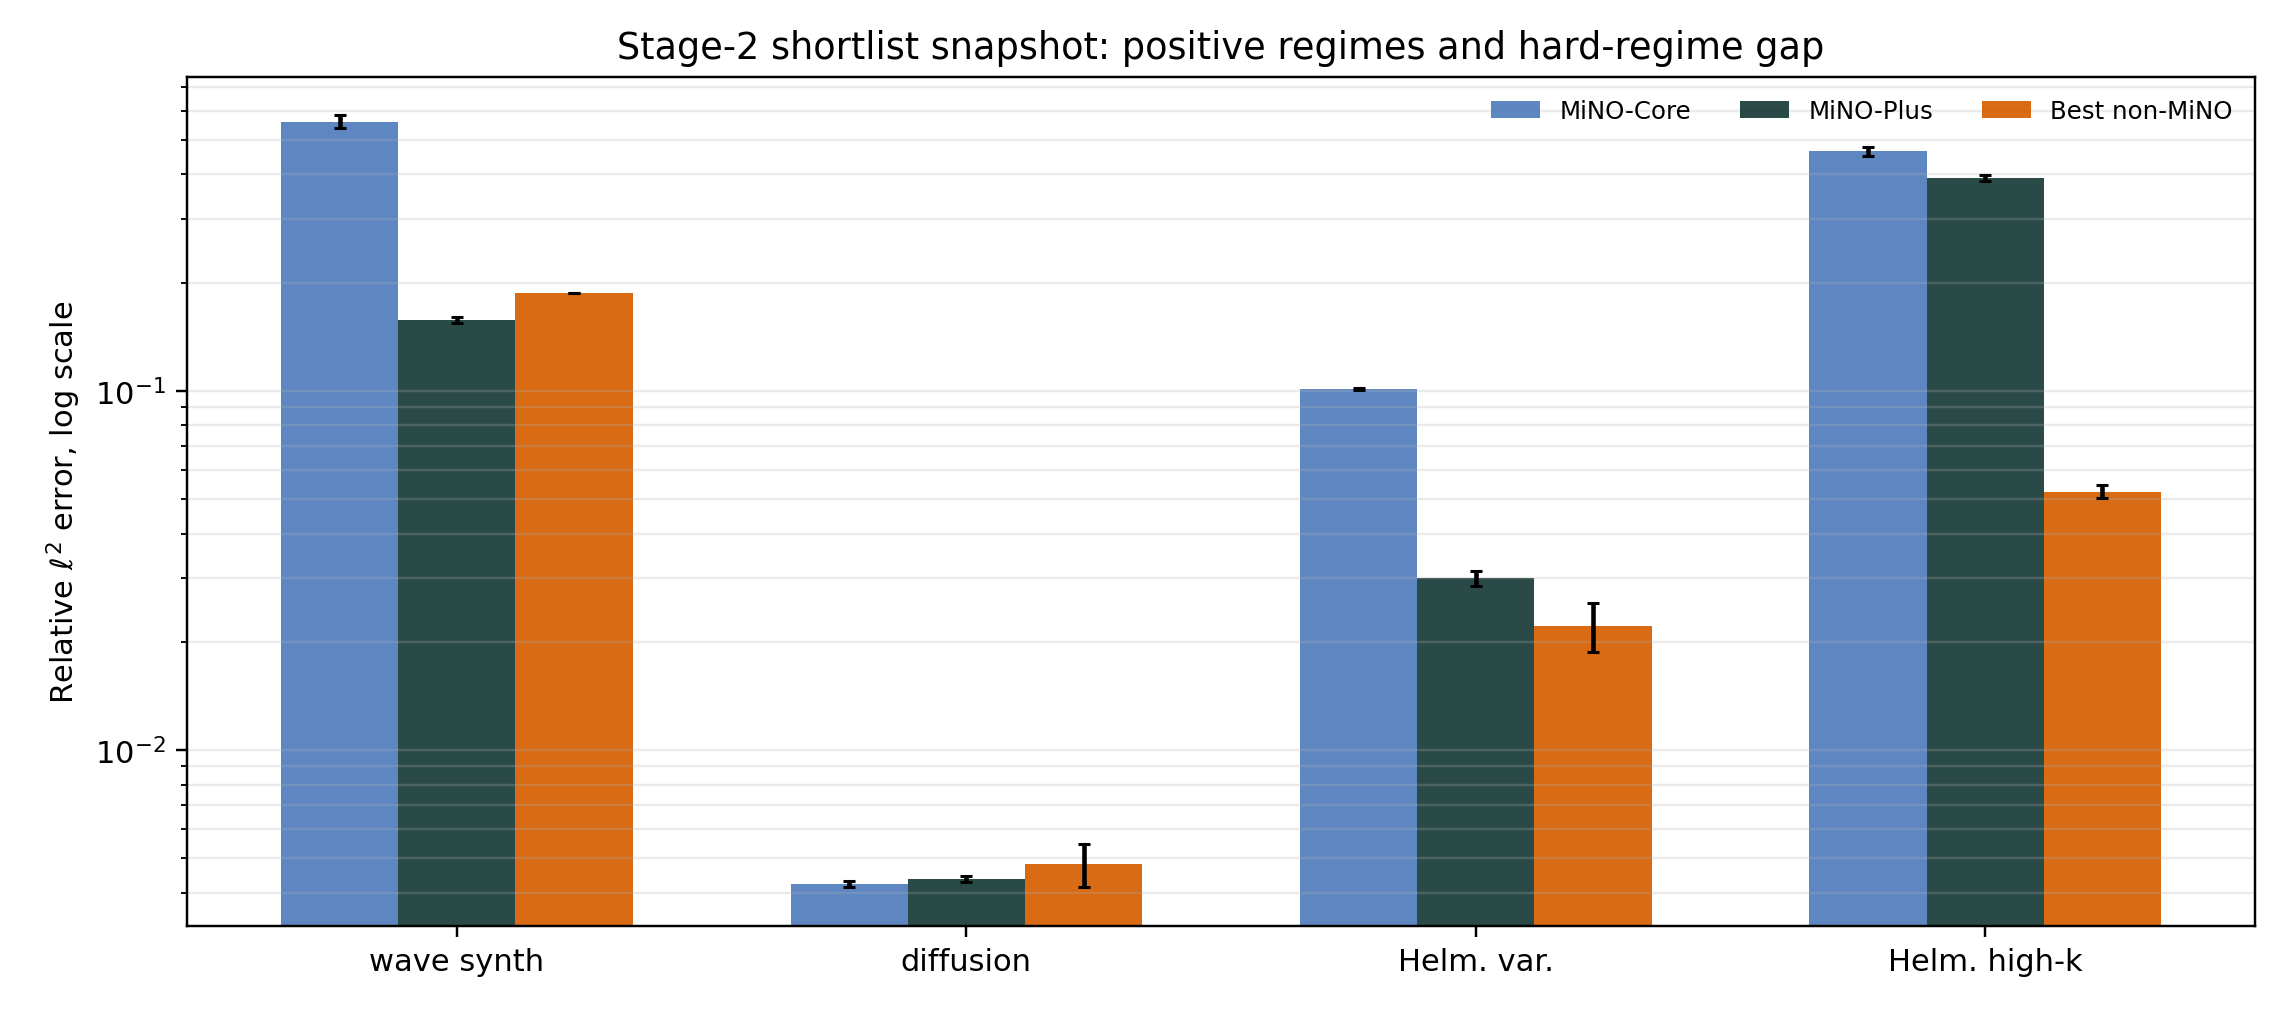
\includegraphics[width=0.96\textwidth]{figures/stage2_regime_snapshot.png}
\caption{Stage-2 shortlist snapshot.  The plot puts the positive rows and the high-$k$ Helmholtz motivation on the same log-scale axis.  \MiNO-Plus improves over \MiNO-Core on the wave and Helmholtz rows and is competitive on diffusion; the high-$k$ row motivates the branch/resolvent extension rather than serving as the main mechanism claim.}
\label{fig:stage2-regime-snapshot}
\end{figure}

\subsection{Branched High-\texorpdfstring{$k$}{k} Helmholtz Probe}
\label{sec:branched-helmholtz}

The high-$k$ Helmholtz row is the regime in which a single canonical graph is least plausible.  We therefore add a targeted finite-branch probe for Helmholtz.  The model uses $L=3$ independently parameterized canonical branches, token-wise metadata-softmax routing, branch entropy/diversity regularization, branch-summed transported synthesis and carrier paths, and the same admissible learned finite-landing layer used in the carrier-bound wave controls.  The default \MiNO\ model remains the $L=1$ carrier-bound architecture; the branched profile is used for the \texttt{helmholtz\_branched\_highk} campaign.

The executed rows are sample-capped and answer a narrow question: whether branch multiplicity alone is the active missing budget before adding the stronger outgoing resolvent-symbol layer.

The ablations are designed to separate finite-branch structure from ordinary transport use.  \texttt{single\_branch} forces the router onto branch 1 at fixed architecture, \texttt{no\_branch\_routing} replaces the learned router by uniform routing, \texttt{no\_transport} removes branch transport, \texttt{no\_transport\_no\_carrier} additionally removes transported synthesis/carrier/landing, and \texttt{no\_symbol} removes symbol modulation.  The criterion is conservative: a useful branch result should reduce the high-$k$ gap relative to the single-branch row, and otherwise the row is treated as a guide for the next microlocal budget rather than as a central claim.

The sample-capped branch-only result serves as a budget-local branch probe.  Across the three Helmholtz rows, the full $L=3$ branched model is close to the forced single-branch model, the uniform-routing ablation, and the no-symbol ablation.  This points to a sharper implementation requirement already predicted by the calculus ledger: branch multiplicity alone is too weak unless the frame, router, phase/landing, and outgoing resolvent-symbol budgets are all controlled.  The full table, routing plot, and field panels are kept in Appendix~\ref{app:diagnostic-figures}; the main text uses the row to motivate the \texttt{helmholtz\_resolvent} extension.

The follow-up \texttt{helmholtz\_highk\_careful} profile is therefore theory-aligned differently: it keeps the anisotropic packet frame and carrier-bound landing path, but replaces the generic \texttt{spectral\_order} multiplier by the executable \texttt{helmholtz\_resolvent} symbol layer from Corollary~\ref{cor:helmholtz-resolvent-symbol-budget}.  The layer uses an auto-calibrated shell and finite complex-pair multiplication for the signed outgoing resolvent factor, so the comparison is no longer merely an envelope-only symbol ablation.  Table~\ref{tab:helmholtz-highk-careful-midscale} reports the completed local mid-scale row and two matched profile checks.  Increasing the finite packet/resolvent capacity from the minimal smoke profile reduces the high-$k$ relative $\ell^2$ error from roughly $0.71$ to $0.50$.  The ablations also delimit the mechanism: forcing a single branch leaves the result unchanged, and removing the transport message alone is nearly flat, while removing both transport and the transported high-frequency carrier degrades strongly.  The \texttt{no\_symbol} row is close in relative $\ell^2$ and can be slightly better at some finite budgets, while its phase-sensitive diagnostics are worse; the matched \texttt{spectral\_order} row has essentially the same relative $\ell^2$ but worse phase than \texttt{helmholtz\_resolvent}.  The safe reading is therefore that the outgoing symbol layer is active and phase-sensitive, but is not yet a standalone relative-$\ell^2$ improvement.  The runner now separates this budget into \texttt{source\_only\_symbol}, \texttt{no\_edge\_symbol}, and \texttt{no\_resolvent\_phase} rows, with a small symbol-identity regularizer available when the local-kernel correction should remain a diagnostic rather than a default field-error path.  The matched \texttt{gabor\_gaussian} row has lower phase error but substantially worse relative $\ell^2$, so the high-$k$ field-error gain is attributed primarily to anisotropic packet resolution plus carrier-bound landing rather than to the isotropic Gabor frame.  Thus the current high-$k$ evidence supports anisotropic carrier-bound reconstruction more strongly than multibranch canonical transport, with the resolvent/local-kernel symbol remaining a phase/radiation budget under refinement.

\begin{table}[t]
\centering
\caption{Mid-scale \texttt{helmholtz\_highk\_careful} probe on \texttt{helmholtz\_highk\_positive}. Entries are three-seed means with standard deviations. The ablation block uses anisotropic packets, the \texttt{helmholtz\_resolvent} complex-pair symbol layer, two canonical branches, width 48, six modes, a transported landing decoder with eight channels, and 16 training epochs. The matched-profile block changes one calculus hook at a time. Lower is better.}
\label{tab:helmholtz-highk-careful-midscale}
\small
\begin{tabular}{lccc}
\toprule
Ablation & Rel. $\ell^2$ & Phase error & Imaginary resolvent energy \\
\midrule
\texttt{full} & $0.503\pm0.008$ & $1.511\pm0.028$ & $0.0349$ \\
\texttt{single\_branch} & $\mathbf{0.502}\pm0.005$ & $1.512\pm0.008$ & $0.0322$ \\
\texttt{no\_transport} & $0.506\pm0.011$ & $\mathbf{1.509}\pm0.006$ & $0.0229$ \\
\texttt{no\_transport\_no\_carrier} & $0.842\pm0.002$ & $1.499\pm0.015$ & $0.0424$ \\
\texttt{no\_symbol} & $0.509\pm0.012$ & $1.602\pm0.022$ & $0.0000$ \\
\bottomrule
\end{tabular}

\vspace{0.6em}
\begin{tabular}{lcc}
\toprule
Matched full-model profile & Rel. $\ell^2$ & Phase error \\
\midrule
\texttt{anisotropic\_gabor} + \texttt{helmholtz\_resolvent} & $0.503\pm0.008$ & $1.511\pm0.028$ \\
\texttt{anisotropic\_gabor} + \texttt{spectral\_order} & $\mathbf{0.502}\pm0.007$ & $1.609\pm0.037$ \\
\texttt{gabor\_gaussian} + \texttt{helmholtz\_resolvent} & $0.584\pm0.017$ & $\mathbf{1.486}\pm0.014$ \\
\bottomrule
\end{tabular}
\end{table}


\paragraph{Flagship high-frequency contract.}
The mid-scale row is not the full high-$k$ claim.  The registered flagship protocol is stricter: train on moderate frequencies, test on larger $k$, report nondimensional frequency $kL$, wavelengths across the domain, points per wavelength, reference-solver residual, complex relative $\ell^2$ when real/imaginary channels are present, amplitude and phase error, PDE residual, boundary/radiation residual, receiver or far-field trace error when available, runtime, memory, and error degradation as $k$ increases.  The runner now logs three finite proxies for this contract in addition to relative $\ell^2$: \texttt{test\_complex\_relative\_l2\_proxy}, which uses genuine real/imaginary channel pairs when the dataset supplies them; \texttt{test\_amplitude\_error\_proxy}, which measures envelope mismatch; and \texttt{test\_boundary\_trace\_error\_proxy}, which records a receiver-style boundary trace mismatch.  The baseline set is also tiered.  General neural operators (FNO, UNO/U-FNO, WNO, CNO/CANO-style attention when available) test whether the packet matrix improves over generic operator primitives.  Helmholtz-specialized solvers, including neural multigrid/Fourier and probabilistic high-frequency Helmholtz references, are required before claiming competitiveness in the high-$k$ solver literature.  The runner exposes this as \texttt{helmholtz\_highk\_flagship}; the campaign uses anisotropic packets, carrier-bound finite landing, \texttt{helmholtz\_resolvent}, OOD high-$k$ rows, and explicit complex-pair losses only when the dataset provides real/imaginary channels.  This protocol is the path from the current mechanism evidence to a high-$k$ flagship benchmark.

\subsection{Carrier-Bound Branch Identifiability}

The final \MiNO\ mechanism test is the carrier-bound \texttt{branch\_id\_v3} profile.  It keeps packet metadata batch-specific, uses Hamiltonian St\"ormer--Verlet metadata transport, synthesizes learned coefficients at transported packet centers, and adds a transported high-frequency input carrier from the original packet coefficients.  Skip and refinement paths are low-pass restricted, token-level refinement is disabled, and controlled-flow rows use the known packet drift as a metadata-flow target.  This makes transport a field-level mechanism: disabling transport leaves the high-frequency carrier at the analysis centers rather than the learned transported centers.

For fairness, the ablations are defined at the executable level.  \texttt{no\_transport} zeroes the propagation message and keeps identity metadata; it does not randomize packet centers.  \texttt{identity\_transport} keeps the propagation/message path but freezes displacement.  \texttt{randomized\_metadata} permutes metadata across packets, preserving the metadata multiset while breaking the packet--metadata association.  The same-refinement baseline column uses the same low-pass image-space refinement mechanism and training loss budget as \MiNO-Plus, but without MiNO's packet tokenizer, transported synthesis, transported carrier, or token-level packet refinement.  The registered \texttt{branch\_id\_v3\_controls} campaign adds two fairness controls: \texttt{full\_no\_flow\_supervision}, which removes metadata-flow supervision at fixed architecture, and \texttt{no\_transport\_no\_carrier}, which removes both transport and the transported high-frequency carrier.  These controls separate flow-supervision dependence, carrier binding, and learned transport corruption.

\begin{table}[t]
\centering
\caption{Carrier-bound \texttt{branch\_id\_v3} mechanism test. Entries are mean relative $\ell^2$ over three seeds; lower is better. Scenario aliases match the five controlled wave rows listed in the text.}
\label{tab:branchidv3}
\small
\scriptsize
\begin{tabular}{@{}p{0.16\textwidth}ccccc@{}}
\toprule
Scenario & \MiNO & No transport & Random metadata & No symbol & Best same-refine \\
\midrule
bichar. & 0.380 & 0.714 & 0.912 & 0.395 & 0.056 (UNO) \\
chirp & 0.316 & 0.839 & 1.048 & 0.335 & 0.070 (UNO) \\
two-packet & 0.204 & 0.777 & 1.037 & 0.236 & 0.022 (UNO) \\
var-speed & 0.239 & 0.456 & 0.890 & 0.240 & 0.074 (UNO) \\
wave synth & 0.295 & 0.537 & 0.900 & 0.298 & 0.154 (UNO) \\
\bottomrule
\end{tabular}
\end{table}

The controls table below is generated from the completed \texttt{branch\_id\_v3\_controls} summary.  It is the fairness counterpart to Table~\ref{tab:branchidv3}: \texttt{full\_no\_flow\_supervision} tests whether the effect is merely flow-supervision driven, and \texttt{no\_transport\_no\_carrier} tests whether the degradation is explained by the transported carrier path alone.  Across all five rows, removing flow supervision changes relative $\ell^2$ by at most $0.020$, while removing transport increases relative $\ell^2$ by $0.217$--$0.574$.  Removing both transport and the high-frequency carrier remains worse than the full model in every row, and is worse than \texttt{no\_transport} in four of the five rows.

\begin{table}[t]
\centering
\caption{Registered \texttt{branch\_id\_v3\_controls} field-error checks. Entries are mean relative $\ell^2$ over three seeds; lower is better.}
\label{tab:branchidv3controls}
\scriptsize
\begin{tabular}{lccccccc}
\toprule
Scenario & Full & No flow & No tr. & Identity & No tr./car. & Rand. meta & No sym. \\
\midrule
bichar. & 0.378 & 0.379 & 0.715 & 0.714 & 0.815 & 0.912 & 0.392 \\
chirp & 0.315 & 0.319 & 0.840 & 0.806 & 0.826 & 1.044 & 0.334 \\
two-packet & 0.205 & 0.185 & 0.779 & 0.749 & 0.801 & 1.038 & 0.234 \\
var-speed & 0.238 & 0.238 & 0.455 & 0.456 & 0.753 & 0.892 & 0.240 \\
wave synth & 0.296 & 0.296 & 0.534 & 0.535 & 0.774 & 0.905 & 0.298 \\
\bottomrule
\end{tabular}
\end{table}


The ablation pattern is coherent.  Removing transport increases field error in every row; identity transport behaves like the transport-off control; randomizing metadata increases the error further; removing only the symbol branch has a smaller effect on these transport-dominant wave probes.  The same-refinement baselines are included as absolute-accuracy controls.  Tables~\ref{tab:branchidv3}--\ref{tab:branchidv3controls} therefore establish the main empirical point: the final \MiNO\ architecture uses packet transport as a causal field-level branch under the registered carrier-bound protocol.

\begin{table}[t]
\centering
\caption{Theorem-to-metric map for the carrier-bound mechanism evidence.  The table records what each theorem budget predicts experimentally and which registered row probes it.}
\label{tab:theorem-metric-map}
\scriptsize
\begin{tabular}{p{0.22\textwidth}p{0.27\textwidth}p{0.27\textwidth}p{0.13\textwidth}}
\toprule
Theorem term & Artifact metric & Registered probe & Status \\
\midrule
Transport budget $E_{\mathrm{tr}}$ & relative $\ell^2$, canonical-flow proxy, WF-transport proxy & \texttt{no\_transport}, \texttt{identity\_transport}, \texttt{randomized\_metadata} & tested \\
Transported synthesis $E_{\mathrm{tsyn}}$ & field error under transported synthesis corruption & \texttt{identity\_transport} vs full & tested \\
Carrier channel $E_{\mathrm{car}}$ & extra degradation after removing transported carrier & \texttt{no\_transport\_no\_carrier} vs \texttt{no\_transport} & tested \\
Symbol budget $E_{\mathrm{sym}}$ & relative $\ell^2$, symbol-order proxy & \texttt{no\_symbol} & tested \\
Packet tail $E_{\mathrm{tail}}$ & packet-WF localization and future $K$ sweep & fixed-$K$ controls; budget sweep deferred & partial \\
Frame/asymptotic/covering $E_{\mathrm{frame}},E_{\mathrm{asymp}},\delta_h$ & tokenizer reconstruction, frame diagnostics, resolution sweep & cross-resolution campaign & deferred \\
\bottomrule
\end{tabular}
\end{table}

This table also fixes the interpretation of the mechanism claim.  Field degradation under transport corruption is a causal-use test.  On controlled rows we additionally log canonical-flow and packet-wavefront proxies; budget-scaling in $K$, transport capacity, symbol capacity, and packet resolution is the natural quantitative follow-up.

\paragraph{Executable landing diagnostic.}
The theory idealizes a packet synthesis operator with controlled frame constants, while the executable model must land transported packet content on a finite pixel grid.  We therefore ran a synthesis-mode probe on the two cleanest wavefront scenarios.  Two analytic replacements for the packet-energy warp, moved Gabor-atom splatting and moved local-patch folding, were substantially worse.  A transport-conditioned finite landing decoder was the only tested landing map that reduced the UNO gap in the single-seed diagnostic, reaching relative $\ell^2$ $0.056$ on \texttt{wave\_chirp\_propagation} and $0.034$ on \texttt{wave\_two\_packet\_no\_interaction}.  The narrow theoretical reading is that the learned decoder reduces the executable landing terms $E_{\mathrm{tsyn}}$ and $E_{\mathrm{car}}$; it does not change the canonical propagation theorem and it is not a new microlocal calculus result.

\begin{table}[t]
\centering
\caption{Single-seed executable landing probe.  This table is diagnostic, not a replacement for the registered three-seed mechanism tables.  It tests whether the remaining UNO gap is partly a finite landing problem rather than a canonical-flow problem.}
\label{tab:synthesis-mode-probe}
\small
\begin{tabular}{p{0.23\textwidth}p{0.18\textwidth}ccc}
\toprule
Scenario & Landing map & Full & No transport & UNO+ref \\
\midrule
chirp & warp & 0.316 & 0.839 & 0.070 \\
 & atom splat & 0.801 & 0.841 & 0.048 \\
 & patch fold & 0.758 & 0.662 & 0.047 \\
 & learned landing & 0.056 & 0.093 & 0.048 \\
\addlinespace
two-packet & warp & 0.204 & 0.777 & 0.022 \\
 & atom splat & 0.680 & 0.836 & 0.021 \\
 & patch fold & 0.764 & 0.743 & 0.022 \\
 & learned landing & 0.034 & 0.053 & 0.022 \\
\bottomrule
\end{tabular}
\end{table}


\begin{figure}[t]
\centering
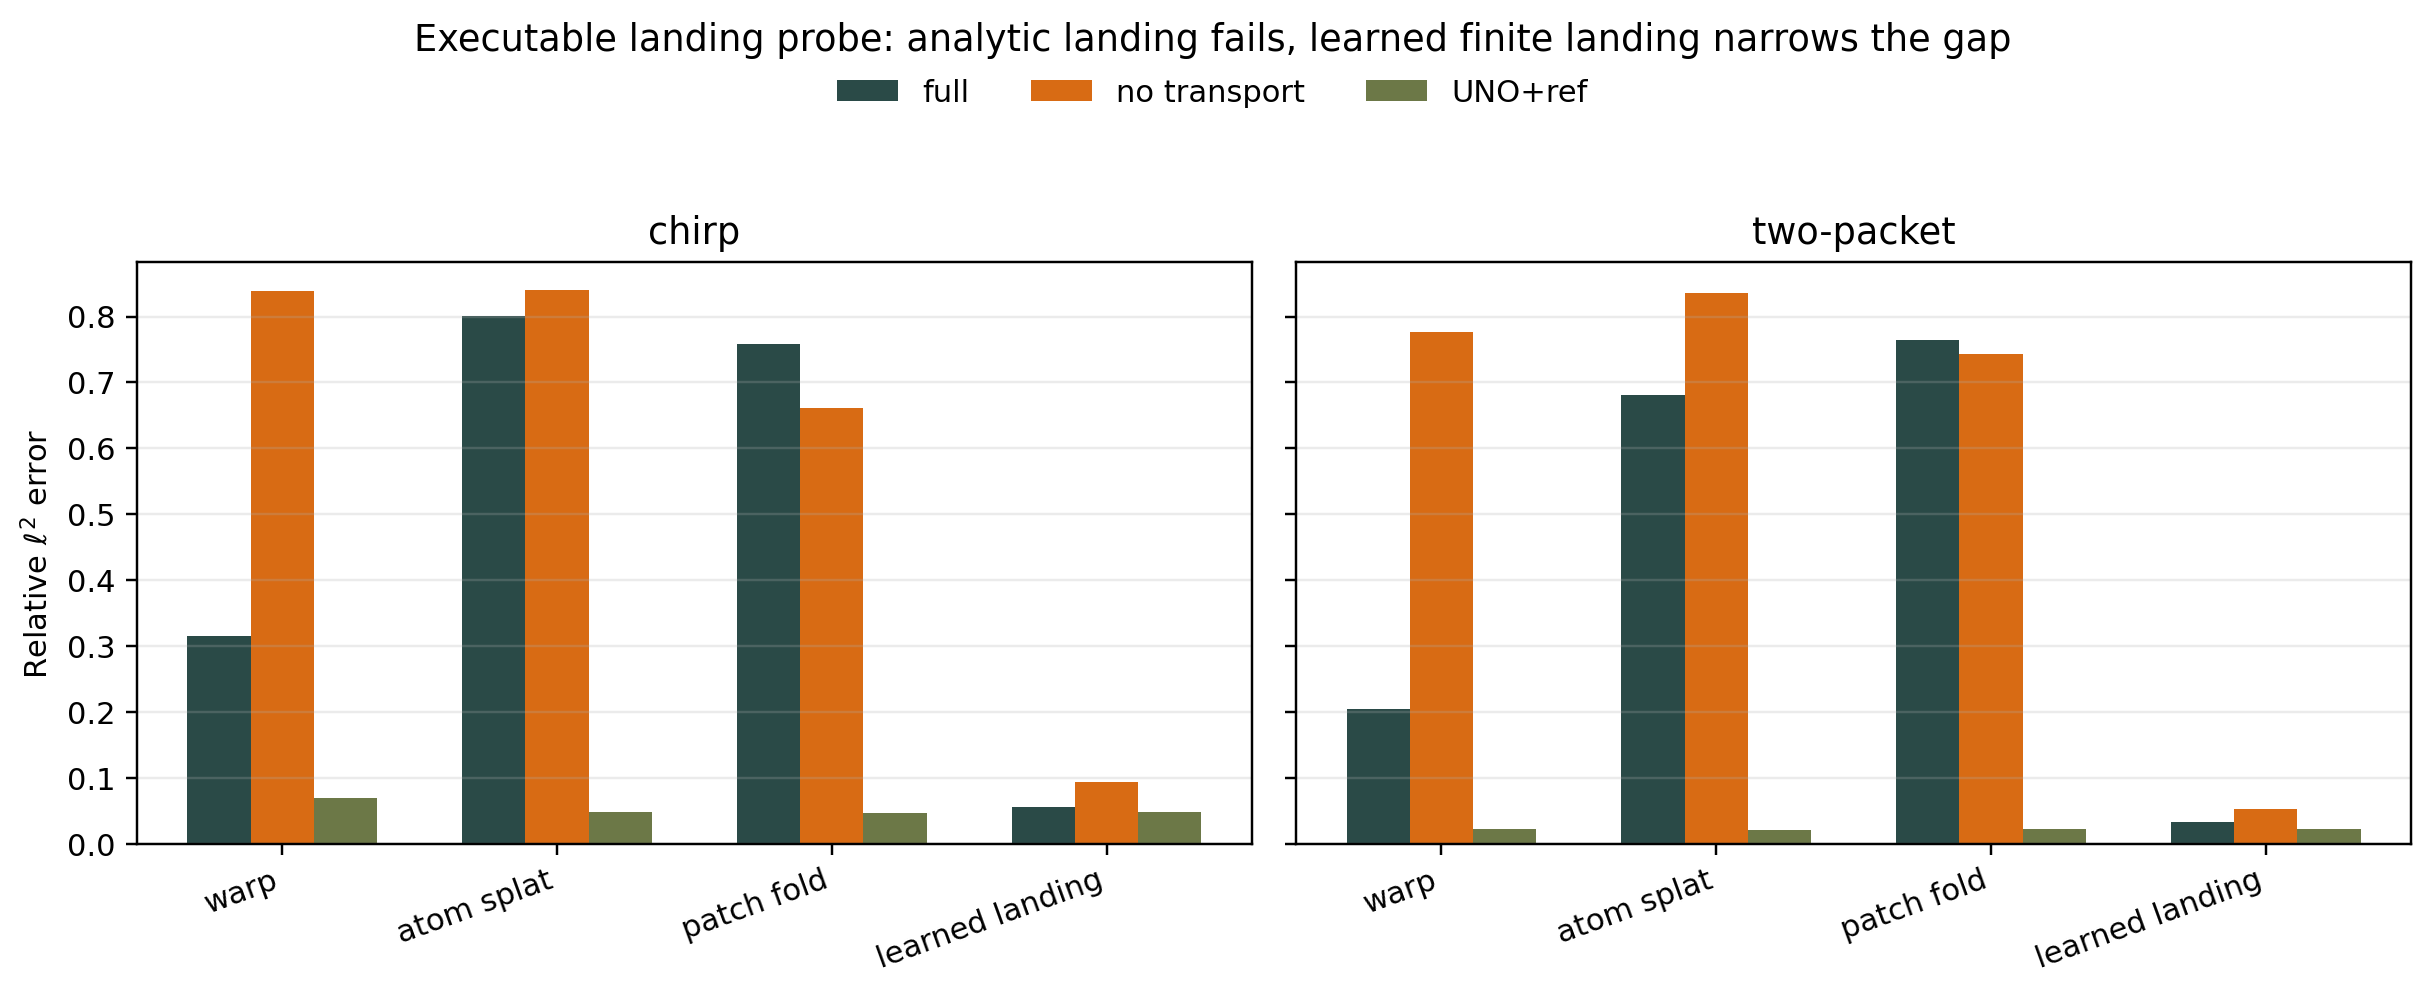
\includegraphics[width=\textwidth]{figures/synthesis_mode_probe_relative_l2.png}
\caption{Single-seed executable landing probe.  The instability of analytic atom-splat and moved-patch folding indicates that the UNO gap is partly an executable finite-landing problem.  The learned landing decoder narrows this gap while preserving a transport ablation penalty, so it is treated as a finite landing layer for $E_{\mathrm{tsyn}}$ and $E_{\mathrm{car}}$.}
\label{fig:synthesis-mode-probe}
\end{figure}

We then promoted the learned finite-landing row to a three-seed \texttt{branch\_id\_v3\_controls} follow-up.  Table~\ref{tab:learned-landing-controls} and Figure~\ref{fig:learned-landing-controls} show the outcome.  The learned landing layer sharply improves absolute field error relative to the analytic finite-landing controls, but it does not erase the transport mechanism: \texttt{no\_transport} remains worse than \texttt{full} in every row, and removing both transport and the high-frequency carrier remains much worse.  The effect is smaller than in the non-decoder carrier-bound table, so the decoder is treated as a finite implementation layer that reduces landing error while preserving a residual transport penalty.  The \texttt{no\_symbol} rows remain flat or slightly better in several scenarios; these learned-landing controls therefore strengthen finite-landing evidence, not symbol-branch attribution.

\begin{table}[t]
\centering
\caption{Three-seed learned finite-landing controls.  Entries are mean relative $\ell^2$; lower is better.  The transport-conditioned decoder reduces absolute field error relative to the analytic finite-landing maps, while transport removal and carrier removal remain visible.}
\label{tab:learned-landing-controls}
\scriptsize
\begin{tabular}{lcccccc}
\toprule
Scenario & Full & No flow & No tr. & No tr./car. & Rand. meta & No sym. \\
\midrule
bichar. & 0.060 & 0.059 & 0.090 & 0.814 & 0.722 & 0.050 \\
chirp & 0.057 & 0.067 & 0.104 & 0.862 & 0.845 & 0.053 \\
two-packet & 0.036 & 0.051 & 0.050 & 0.828 & 0.888 & 0.031 \\
var-speed & 0.072 & 0.086 & 0.144 & 0.754 & 0.752 & 0.101 \\
wave synth & 0.179 & 0.180 & 0.219 & 0.771 & 0.779 & 0.178 \\
\bottomrule
\end{tabular}
\end{table}


\begin{figure}[t]
\centering
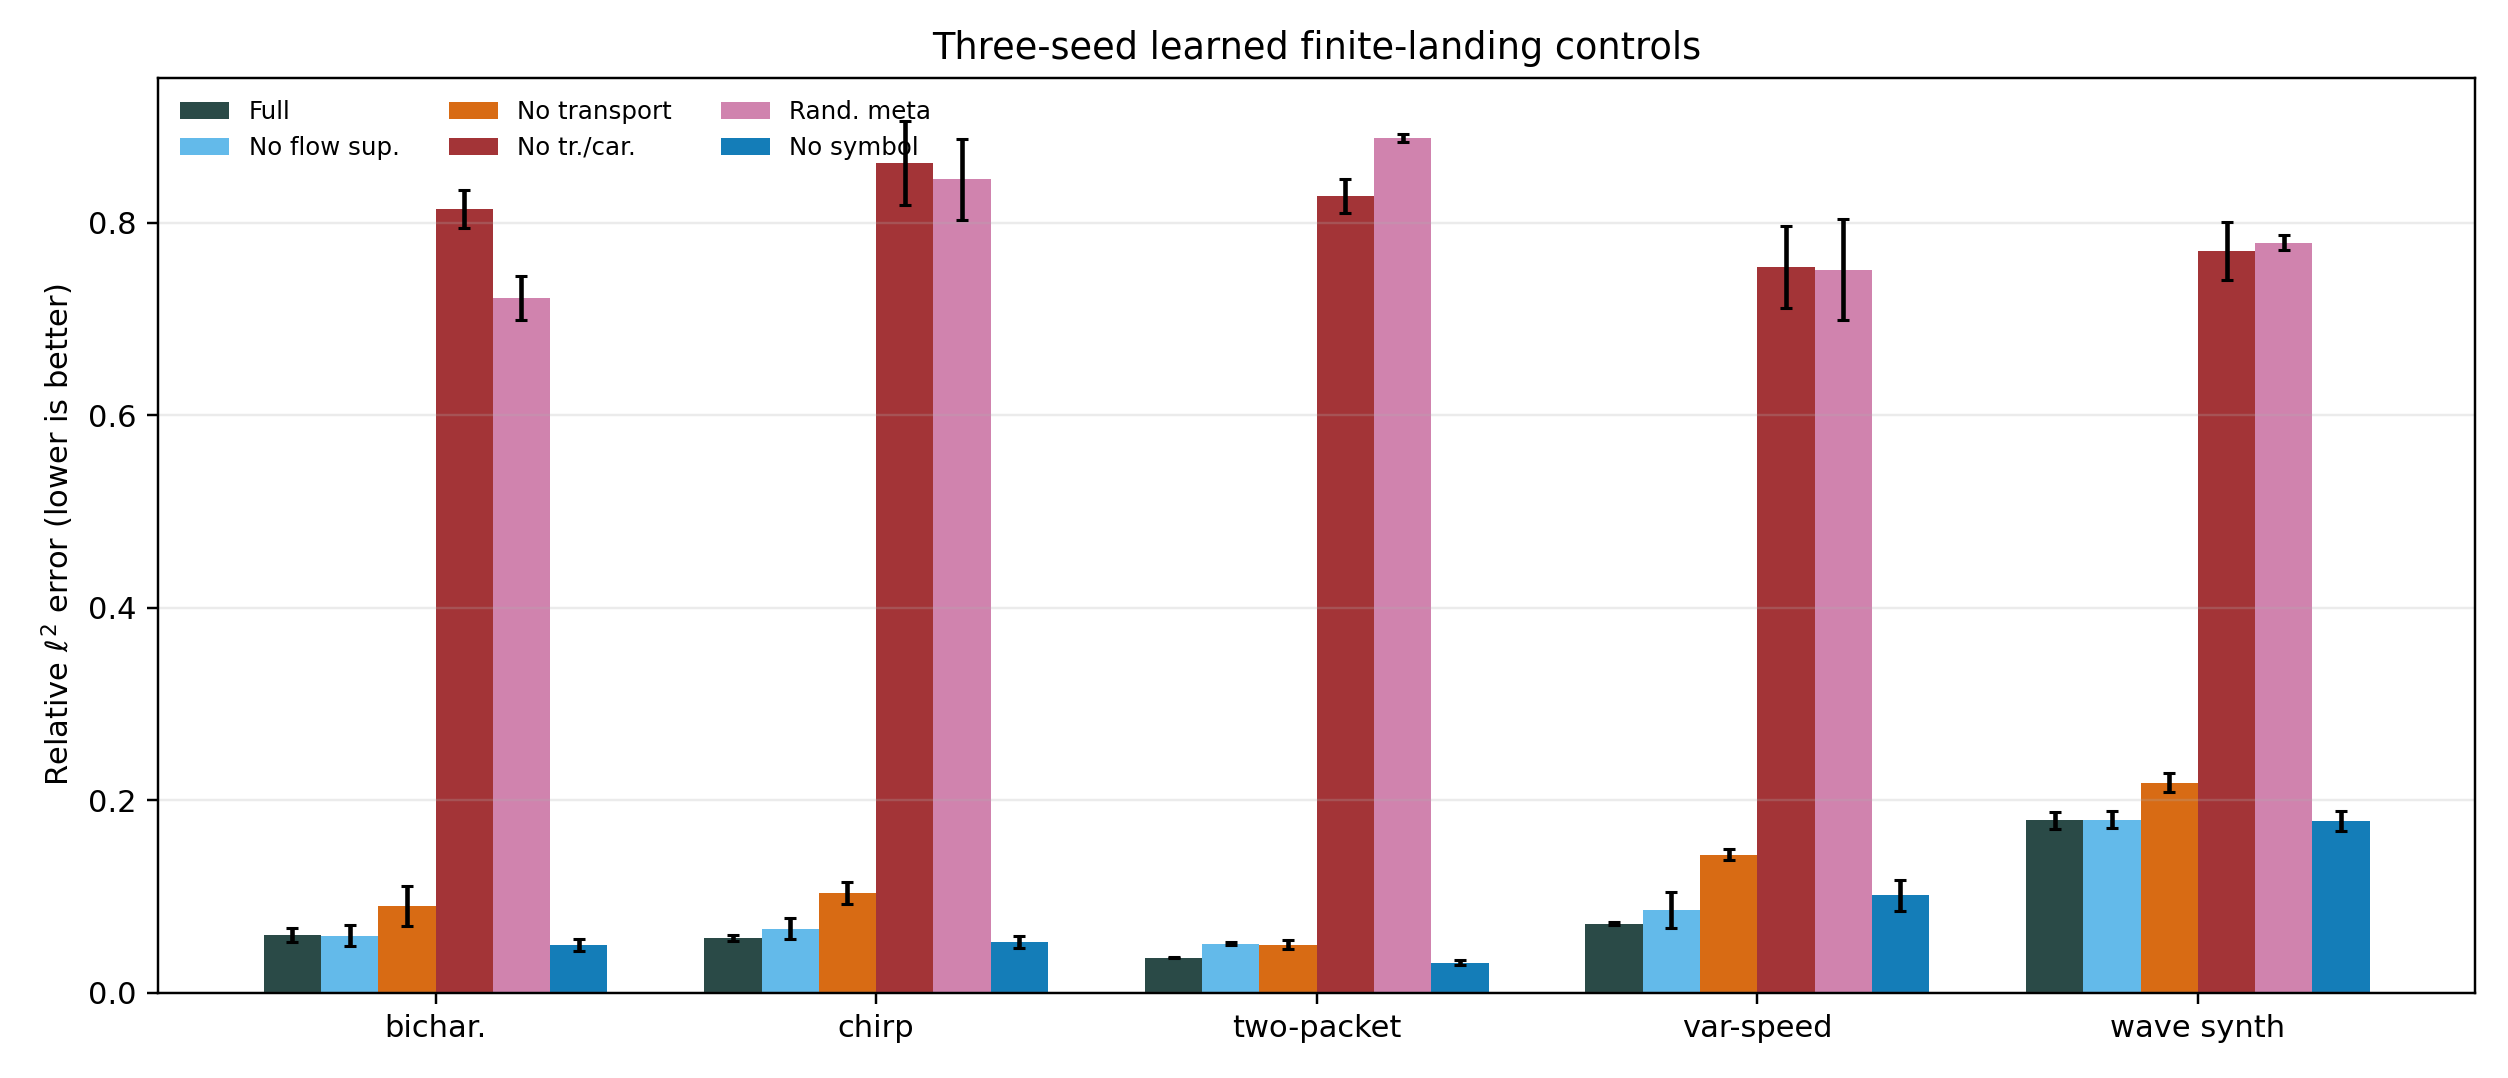
\includegraphics[width=\textwidth]{figures/learned_landing_controls_relative_l2.png}
\caption{Three-seed learned finite-landing controls.  The transport-conditioned decoder reduces absolute field error on controlled wave probes, while \texttt{no\_transport}, \texttt{no\_transport\_no\_carrier}, and metadata randomization remain degraded.  The result supports a finite landing correction that preserves transport dependence.}
\label{fig:learned-landing-controls}
\end{figure}

\begin{figure}[t]
\centering
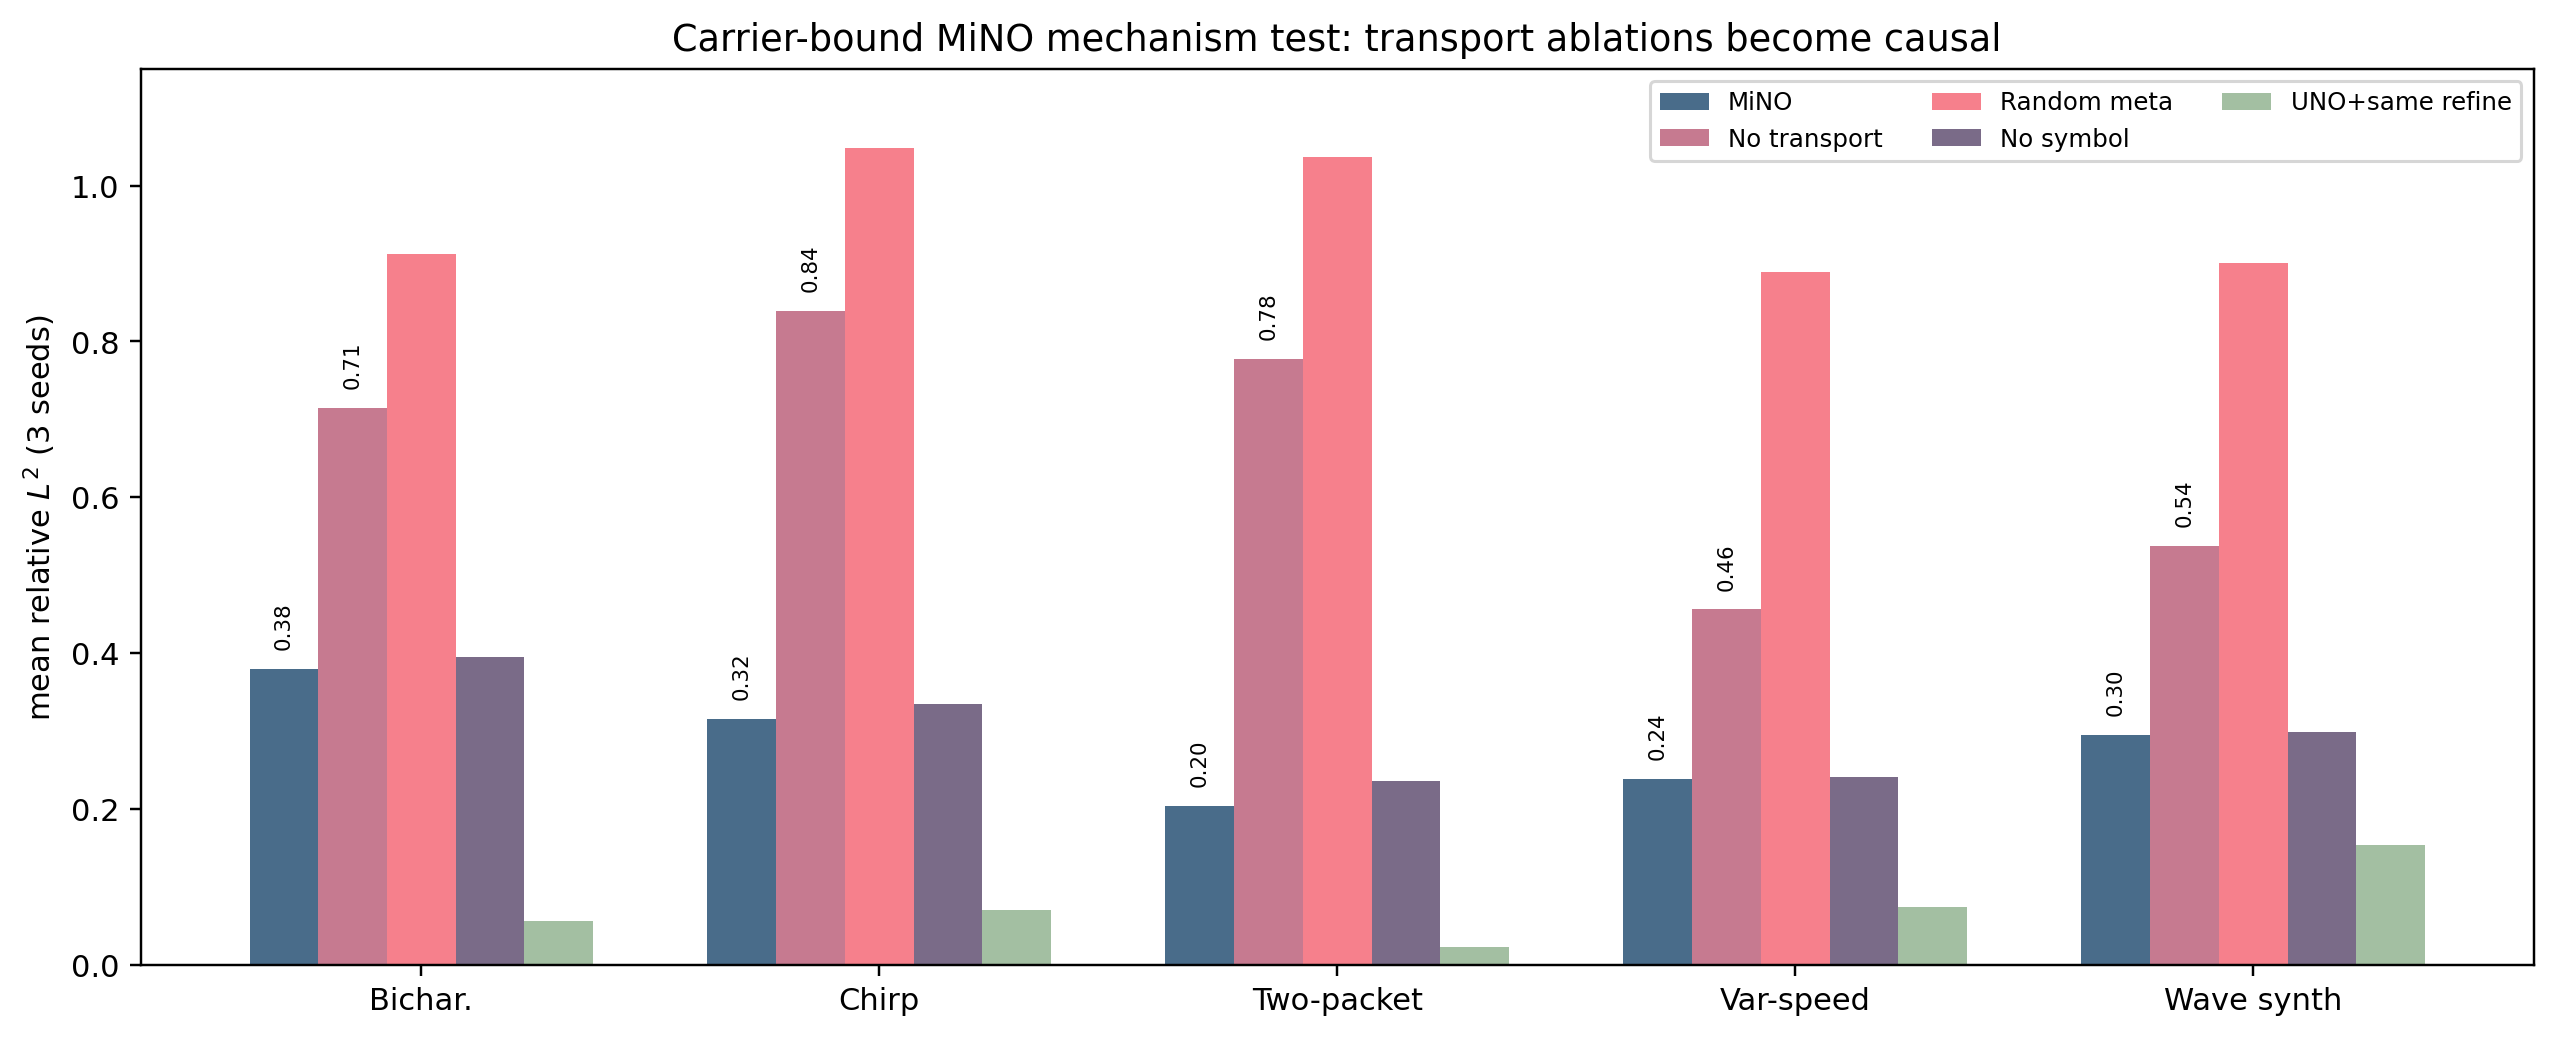
\includegraphics[width=\textwidth]{figures/branch_id_v3_carrier_mechanism_bars.png}
\caption{Carrier-bound branch-identifiability results.  Transport removal and metadata randomization produce a consistent degradation pattern across controlled wave probes, while same-refinement baselines remain a separate absolute-accuracy control.}
\label{fig:branch-id-v3-carrier-bars}
\end{figure}

\begin{figure}[t]
\centering
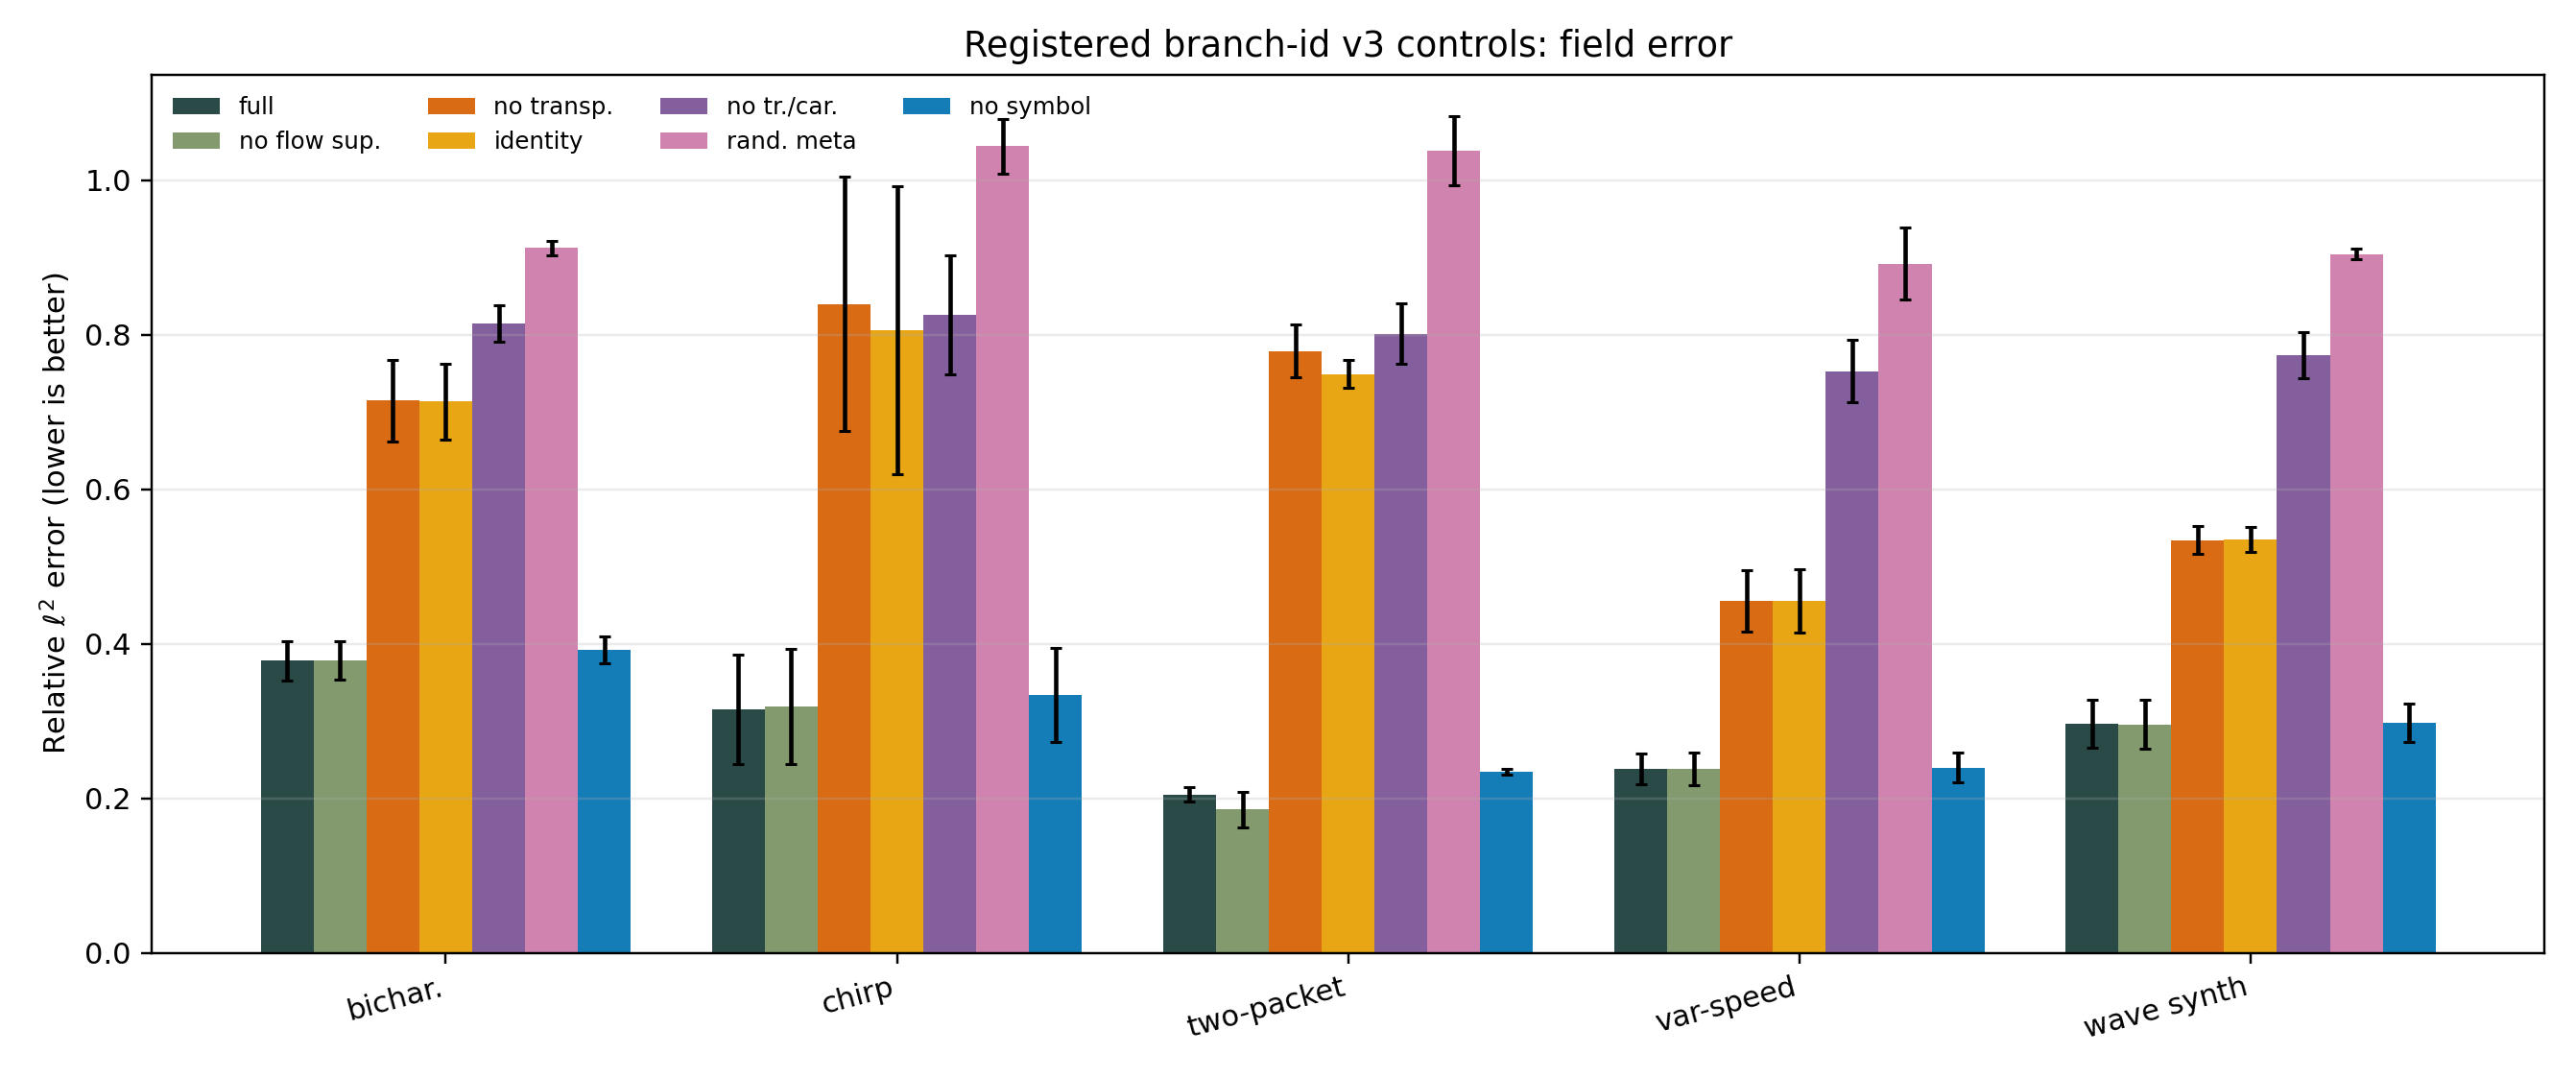
\includegraphics[width=\textwidth]{figures/branch_id_v3_controls_relative_l2.png}
\caption{Registered \texttt{branch\_id\_v3\_controls} field-error checks.  The key comparisons are \texttt{full\_no\_flow\_supervision} versus \texttt{full}, and \texttt{no\_transport\_no\_carrier} versus \texttt{no\_transport}.  Flow supervision is not needed for the reported field-error effect, while carrier removal separates the high-frequency carrier contribution from the transport-corruption contribution.}
\label{fig:branch-id-v3-controls-l2}
\end{figure}

\begin{figure}[t]
\centering
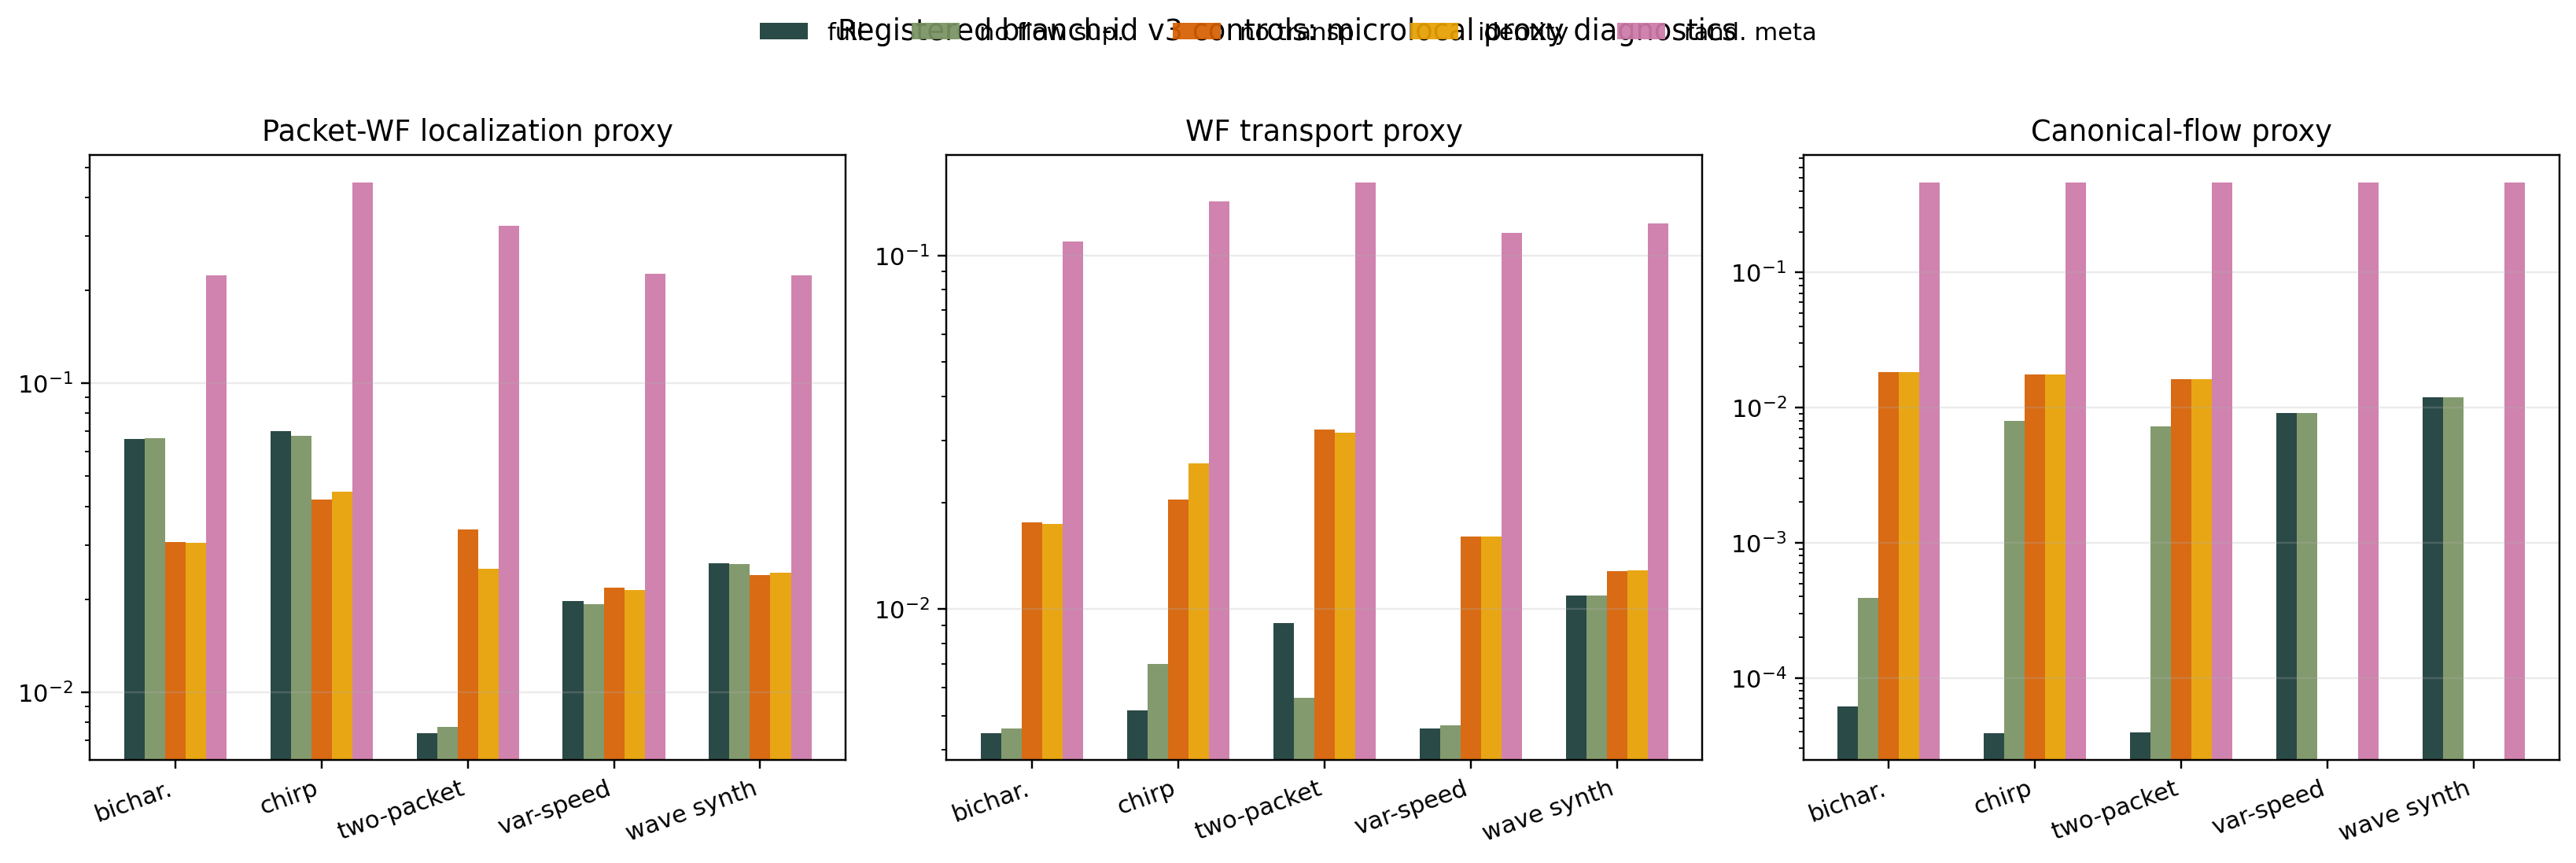
\includegraphics[width=\textwidth]{figures/branch_id_v3_controls_wavefront_proxy.png}
\caption{Registered \texttt{branch\_id\_v3\_controls} microlocal-proxy checks.  The plotted diagnostics correspond to Corollary~\ref{cor:packet-wavefront-localization}: packet-wavefront localization error, wavefront-transport proxy error, and canonical-flow proxy error.  These are mechanism diagnostics rather than aggregate SOTA metrics.}
\label{fig:branch-id-v3-controls-wf}
\end{figure}

\begin{figure}[t]
\centering
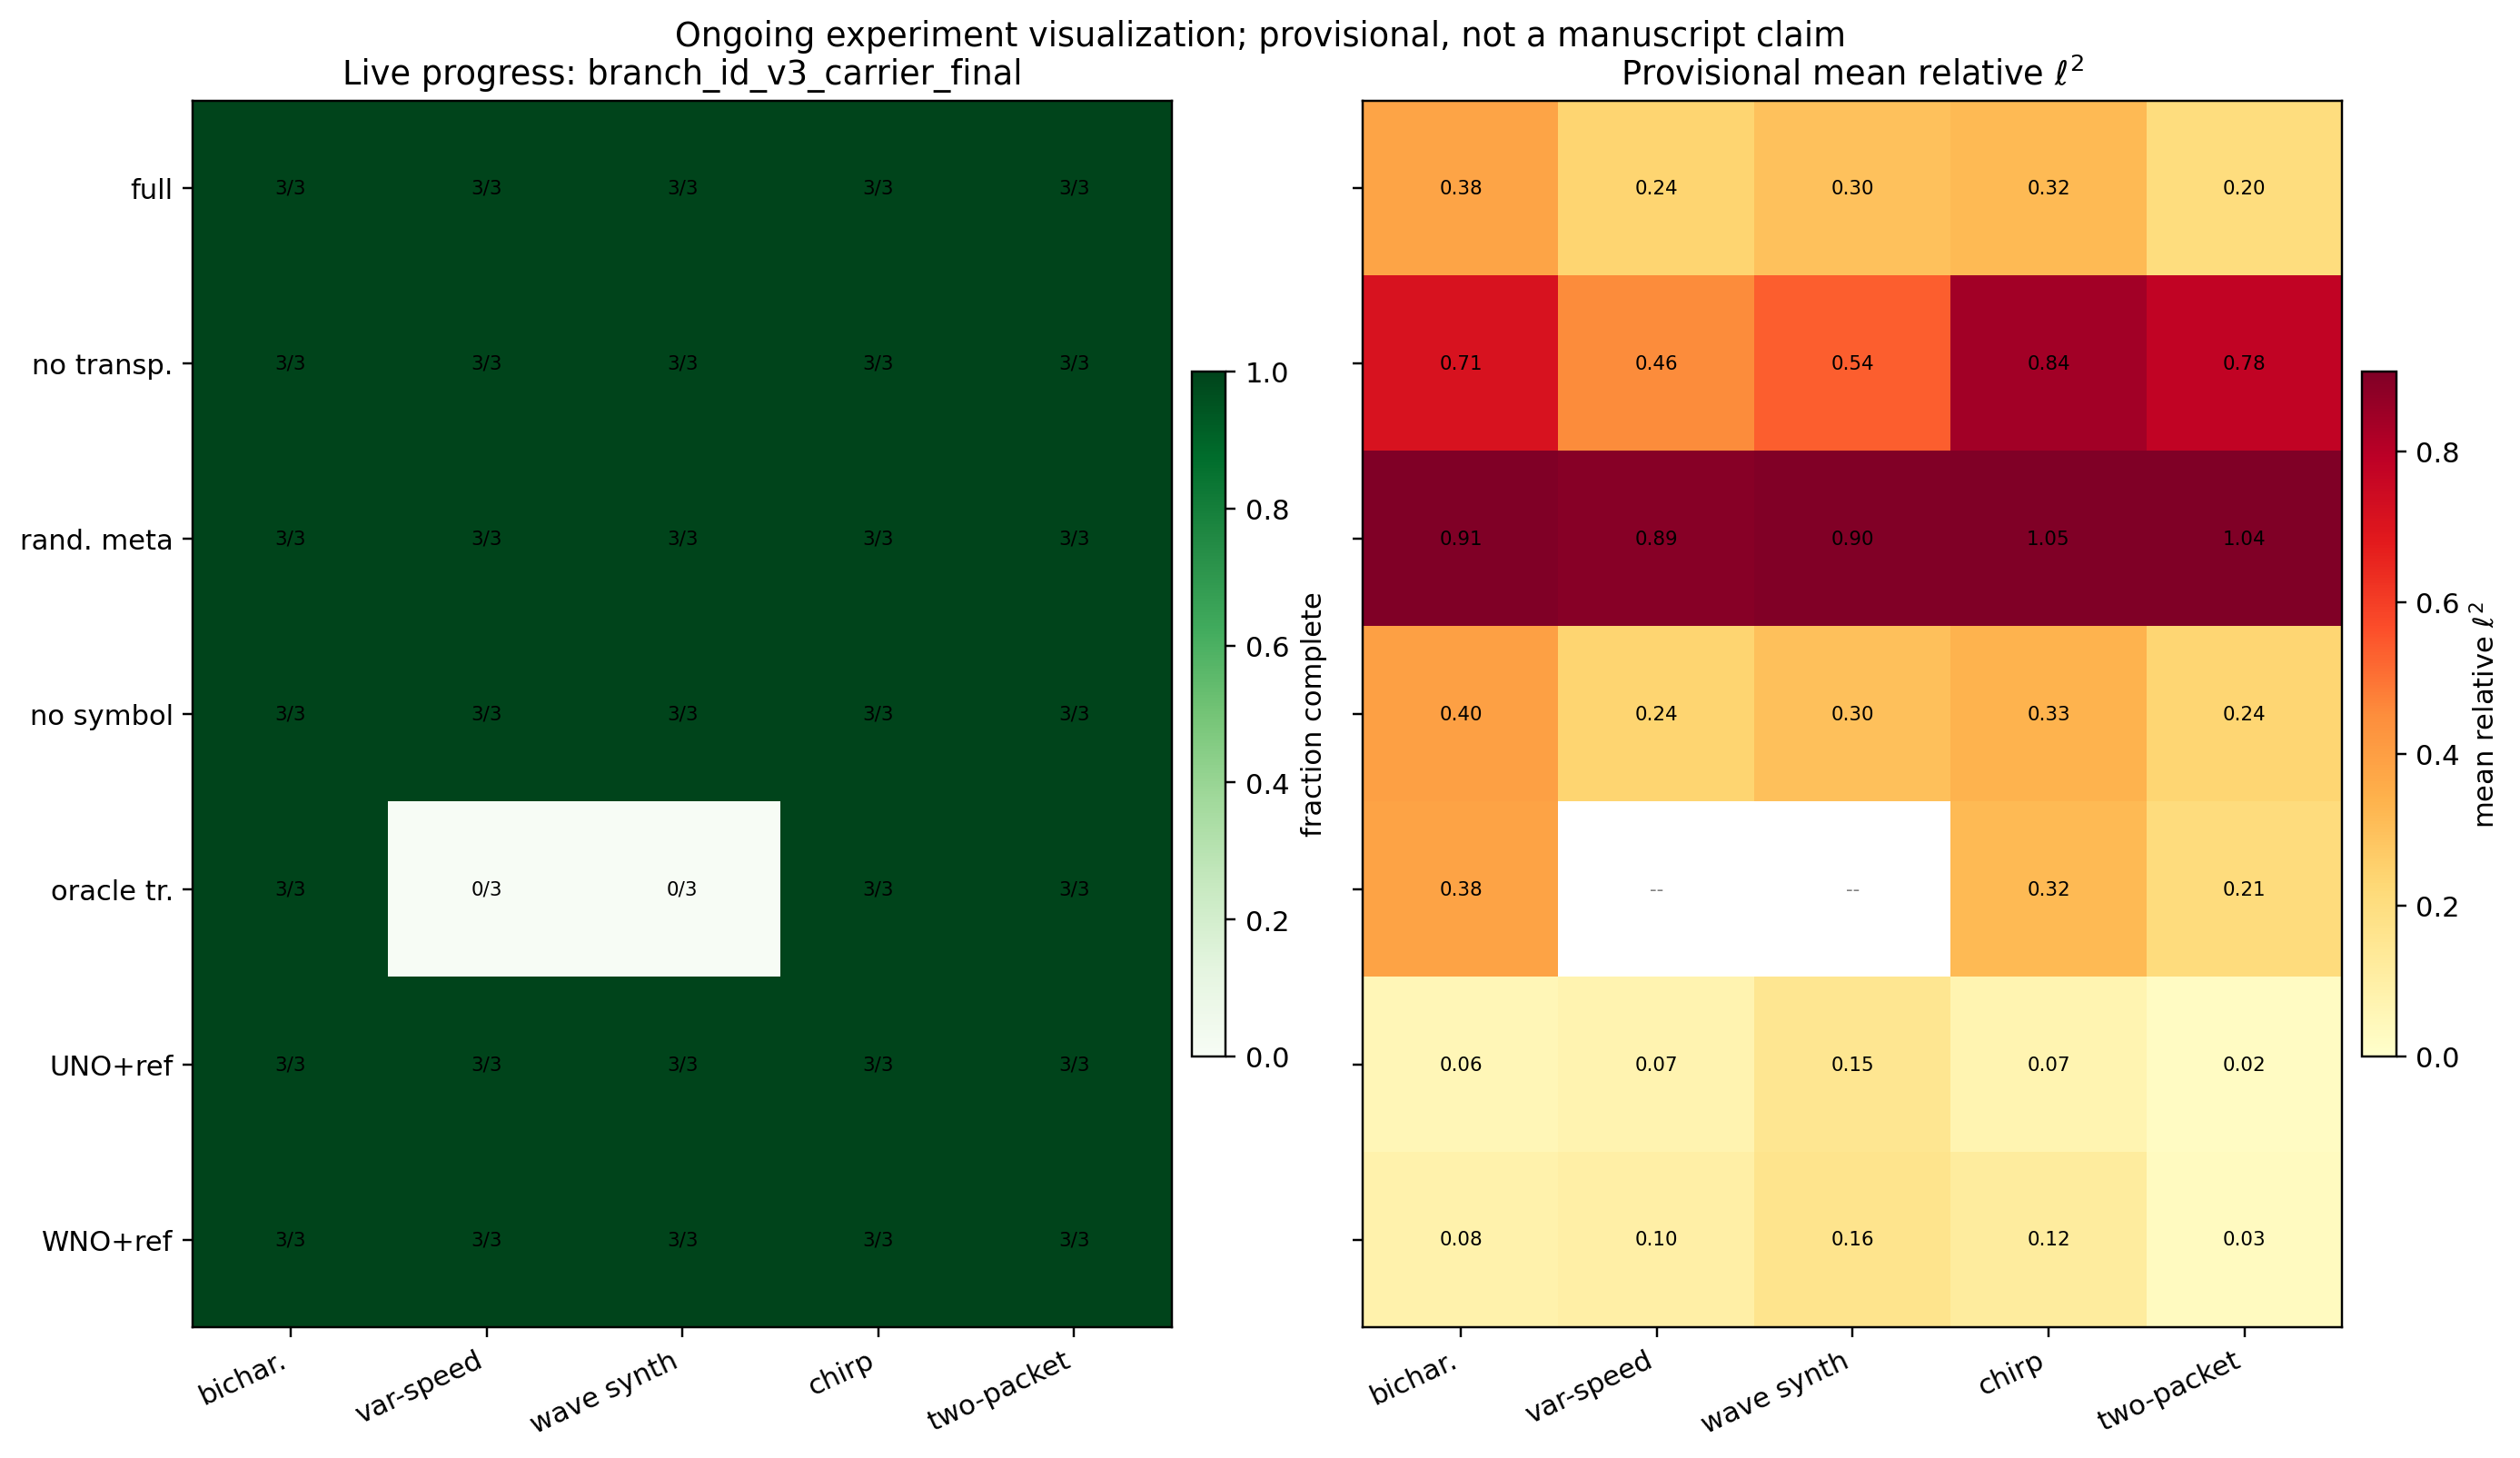
\includegraphics[width=0.92\linewidth]{figures/branch_id_v3_carrier_final_live.png}
\caption{Completed \texttt{branch\_id\_v3} campaign matrix generated by the resumable runner.  Each cell records the completed seed count and the mean relative $\ell^2$ used to build Table~\ref{tab:branchidv3}.}
\label{fig:branch-id-v3-carrier-live}
\end{figure}

\subsection{Claim Matrix}

\begin{table}[t]
\centering
\caption{Claim-to-regime matrix for the carrier-bound \MiNO\ manuscript.}
\label{tab:claimmatrix}
\small
\begin{tabular}{p{0.30\textwidth}p{0.24\textwidth}p{0.32\textwidth}}
\toprule
Claim & Evidence & Verdict \\
\midrule
\MiNO-Core is a theorem-facing packet architecture & $\ell^2$ packet-matrix theorem plus finite Lean landing layer and executable Core model & supported \\
Carrier-bound \MiNO\ makes transport field-causal & branch-ID ablations and controls & supported on controlled wave probes \\
Learned finite landing reduces executable synthesis error & learned-landing controls & supported as finite implementation evidence; transport penalty remains \\
Symbol branch is the dominant wave mechanism & \texttt{no\_symbol} rows & not the dominant effect on these transport-dominant probes \\
Identity/dissipative packet regimes are useful & diffusion rows near strongest imported references & supported as aggregate performance; symbol-branch attribution still requires calculus-regime ablations \\
High-$k$ Helmholtz is a stress diagnostic for anisotropic carrier-bound reconstruction & Table~\ref{tab:helmholtz-highk-careful-midscale} and Corollary~\ref{cor:helmholtz-resolvent-symbol-budget} & local mid-scale improvement; anisotropic packets and carrier-bound landing drive the field-error gain, the resolvent/local-kernel symbol is phase-sensitive but not field-error-positive at every budget, and branch multiplicity is not identified in this row \\
Local-window Helmholtz/Navier probes delimit extension regimes & local-window Helmholtz and synthetic Navier calculus probes & scoping diagnostics for branch/resolvent and transport--diffusion profiles \\
\bottomrule
\end{tabular}
\end{table}

The low-budget local-window Helmholtz and synthetic Navier--Stokes panels are kept as appendix diagnostics (Figures~\ref{fig:helmholtz-navier-calculus-probe}--\ref{fig:helmholtz-navier-prediction-panels}).  They delimit extension regimes and are not part of the main positive evidence.

\subsection{Interpretation}

The empirical evidence aligns with two mechanism statements.  On controlled wave probes, the carrier-bound model makes transported metadata field-causal: transport corruption degrades field error after low-frequency residual paths are restricted.  On the high-$k$ Helmholtz row, the active mechanism is different: the robust field-error signal is carried by anisotropic packet resolution, the transported high-frequency carrier, and finite landing.  The high-$k$ mid-scale ablation does not identify multibranch canonical transport, since \texttt{single\_branch} and \texttt{no\_transport} are essentially flat against \texttt{full}.  The matched profile checks separate the calculus terms: replacing the resolvent/local-kernel symbol changes phase-sensitive behavior more than relative $\ell^2$, while replacing anisotropic packets by isotropic Gabor packets worsens field error.

\section{Artifact and Discussion}
\label{sec:artifact}

\subsection{Artifact}

The executable artifact separates the theorem-facing model, empirical enlargement, benchmark runner, imported references, and Lean finite bridge:
the core paths are \texttt{mino/models/}, \texttt{mino/data/}, \texttt{scripts/}, \texttt{lean/MiNO/Microlocal/}, and \texttt{manuscript/jmlr/}.
The manuscript-source bundle and executable artifact may be distributed separately; an artifact-inclusive bundle contains these paths together with raw JSON/CSV summaries, seed manifests, and exact runner commands.  The Lean component verifies the finite packet landing layer once the classical microlocal estimates have supplied a packet matrix with tails and budgets.  The Python artifact writes raw JSON, aggregate CSV, and manifest files so that benchmark rows can be audited and resumed.

\subsection{Closed Results}

The finite landing spine is closed for the stated packet model: transported-symbol perturbation, bounded-stencil stability, shell/tube truncation, cross-resolution transfer, and the finite landing layer are checked or replayed in the Lean companion.  The operator-level theorem spine is the $\ell^2$ sparse packet-matrix transfer coupled to the continuous no-caustic FIO reduction: short-time half-wave propagation gives a canonical graph, non-stationary phase gives off-tube decay, and packet sparsity converts that decay into a bounded-stencil approximation.  Together these pieces justify carrier-bound \MiNO-Core as a theorem-guided architecture for short-time no-caustic wave propagation.

At the executable level, the theorem-facing \texttt{spectral\_order} branch is aligned with the finite symbol statement: it is a pure multiplier on packet coefficients, while additive feature shifts are assigned to the empirical branch or to residual/landing terms.  For high-$k$ Helmholtz, the artifact exposes \texttt{helmholtz\_resolvent}, a near-characteristic radiation proxy corresponding to Corollary~\ref{cor:helmholtz-resolvent-symbol-budget}.  This branch uses an auto-calibrated shell, signed real/imaginary resolvent weights, an outgoing gate, and a bias-free latent complex-pair action for the signed multiplier.  Repository tests check zero-input equivariance of the theorem-facing symbol output, exact finite real multiplication by complex pairs, and differentiability of the symbol-order proxy with respect to packet values.

\subsection{Mechanism Evidence}

The carrier-bound \texttt{branch\_id\_v3} and \texttt{branch\_id\_v3\_controls} campaigns supply the central mechanism evidence.  They keep final metadata batch-specific, apply transported synthesis by a packet-energy-weighted warp, transport a high-frequency input carrier from the original packet coefficients, low-pass restrict skip and refinement paths, and disable token-level refinement in the binding profile.  Removing metadata-flow supervision leaves field error essentially unchanged; removing transport consistently worsens field error; randomizing metadata worsens it further.  This is the empirical alignment point between the sparse packet-matrix theorem and the carrier-bound executable model.

\subsection{Evidence Boundary}

The completed evidence has a clear center: the sparse canonical packet matrix is a field-level mechanism on controlled short-time wave probes.  The theory identifies the packet operator class, the architecture implements a carrier-bound realization, and the benchmark corrupts the corresponding branch.  The conclusion is primitive-level: when high-frequency content must be landed after nontrivial canonical motion, explicit packet transport is a directly testable representation of the law.  Same-refinement UNO/WNO rows show that strong multiscale baselines can learn useful transported behavior implicitly; \MiNO's contribution is to expose and test that law directly.

The high-$k$ Helmholtz and Navier--Stokes rows serve as calculus stress paths.  For Helmholtz, the local outgoing resolvent requires anisotropic packet resolution, branch separation, phase/landing accuracy, and a near-characteristic radiation symbol.  The \texttt{helmholtz\_branched\_highk} probe shows that branch multiplicity alone is not the active budget at the current scale; the \texttt{helmholtz\_highk\_careful} profile points instead to anisotropic carrier-bound resolvent reconstruction.  For Navier--Stokes-style dynamics, the relevant extension is an advective FIO branch coupled to a dissipative $\Psi$DO branch and pressure/closure residuals.  These rows motivate the extension ledger in Section~\ref{sec:admissible-extension-axes}.

High-$k$ Helmholtz is the most direct future flagship benchmark for the microlocal primitive, because it stresses phase coherence, outgoing radiation, and frequency-scaling rather than generic smooth interpolation.  A solver-level claim requires the stronger contract in Section~\ref{sec:branched-helmholtz}: increasing-$k$ rows, phase and radiation residuals, reference-solver accuracy, and comparisons against both general neural operators and specialized Helmholtz solvers.  Navier--Stokes is a secondary nonlinear stress path; its microlocal hook is transport--diffusion splitting, not a standalone turbulence theory.

Three implementation axes are separated from the main wave theorem.  The separable St\"ormer--Verlet metadata branch gives the cleanest symplectic metadata statement; the main theorem itself only requires a learned near-canonical map with the displayed compact-window error budget.  The local symbol branch is secondary on transport-dominant wave probes and is naturally tested in identity-canonical elliptic, dissipative/parabolic, and outgoing-resolvent regimes.  The learned landing decoder is treated as an admissible finite implementation layer for $E_{\mathrm{land},\theta}$, $E_{\mathrm{tsyn}}$, and $E_{\mathrm{car}}$; transport corruption remains visible after the decoder is enabled.

The extension ledger records how additional microlocal structure enters the same packet budget.  Anisotropic packets, finite multibranch canonical relations, stronger $S^m$ symbol control, outgoing resolvent-symbol enforcement, and nonlinear transport--diffusion coupling each has a packet-calculus object and an executable hook.  Once the hook has a verified finite defect term, it enters the packet-budget theorem additively.

Two foundation directions are separated from the present paper.  An Egorov-style neural calculus would test whether learned operators conjugate pseudodifferential probes by the learned canonical map; the finite objects are $\rho_{\mathrm{Eg},h}^{\mathrm{pkt}}$ for a frozen linear Core and $\rho_{\mathrm{Eg},h}^{\mathrm{Jac}}(u,j)$ for the nonlinear executable model.  An operator-microscopy program would recover and compile a microlocal fingerprint, in the no-caustic graph case $\mathfrak F(T)=(\kappa,S,a,R)$, consisting of canonical map, action/phase primitive, amplitude, and residual.  Multi-chart caustics and Maslov transition data require a separate Lagrangian atlas.

\subsection{Conclusion}

\MiNO\ advances a testable microlocal design principle: neural operators for oscillatory PDEs should expose phase-space packet structure rather than rely only on point-space correlation or global Fourier filtering.  The mathematical contribution is a sparse canonical packet-matrix primitive with a finite machine-checkable landing layer and a short-time wave/FIO approximation theorem for carrier-bound \MiNO-Core.  The empirical contribution is a mechanism-identifiability result: in the carrier-bound architecture, high-frequency reconstruction is tied to transported packet metadata, and transport corruption consistently degrades controlled wave rows.

The resulting claim is specific.  The theorem identifies the operator class, the architecture implements one carrier-bound realization of the transported packet primitive in field synthesis, and the benchmark contract tests whether the trained model uses that primitive.  The high-frequency Helmholtz and Navier--Stokes rows define separate calculus hooks---branch/resolvent structure for outgoing oscillatory inverses and transport--diffusion splitting for nonlinear dynamics---rather than broadening the main mechanism claim.


\appendix
\section{Supplementary Proofs and Derivations}
\label{app:proofs}

\subsection{Proof anatomy of the finite transported-symbol perturbation bound}

The proof of Theorem~\ref{thm:finite-transported-symbol} is short enough to appear in the main text, and its structure reveals what stronger continuous theorems preserve.

\paragraph{Step 1: add and subtract the transported coefficient.}
The only useful algebraic move is to add and subtract the mixed term $\symbolref_i a_{\hat\pi(i)}$. This is what isolates transport error from symbol error.

\paragraph{Step 2: factor the three mechanisms.}
After that addition and subtraction, the difference splits into:
\begin{enumerate}
\item reference symbol times transport mismatch,
\item symbol mismatch times approximate transported coefficient,
\item residual.
\end{enumerate}
This is the whole reason for using a transported-symbol architecture rather than an undifferentiated interaction block.

\paragraph{Step 3: apply envelopes.}
The theorem then requires only the envelope hypotheses on transported coefficients and reference symbol size.

\paragraph{Step 4: sum.}
The $\ell^1$ bound is simply the sum of the pointwise bound over all packets.

The bounded-stencil wave/FIO section preserves the same separation: even when several neighboring packets are retained, the dominant error breaks into transport, symbol, and residual components, summed over a small canonical stencil instead of a single destination.

\subsection{Proof of Proposition~\ref{prop:transplantation}}

The semi-discrete transplantation principle is immediate, but we record its logic in a more explicit way.

Let $K_h$ be a discretized PDE solver and $\mathcal K_h=V_hK_hU_h$ its packet-basis realization. Suppose $\mathcal K_h$ belongs to the transported-symbol class $\mathfrak T(\eps_{\mathrm{tr}},\eps_{\mathrm{sym}},\eps_{\mathrm{res}})$. By definition this means there exists a reference transported-symbol action together with approximate transport, approximate symbol, and residual terms satisfying Assumption~\ref{ass:budgets} for the coefficient vectors of interest. The packet-space map induced by the approximate \MiNO\ layer therefore satisfies the exact hypotheses of Theorem~\ref{thm:finite-transported-symbol}. The coefficient-level error bound follows immediately. No PDE-specific argument is used at this stage; the PDE work is entirely in verifying membership of the packet-basis realization in the transported-symbol class.

\subsection{Proof anatomy of Theorem~\ref{thm:cross-resolution}}

The cross-resolution transfer theorem is finite and introduces a scale-indexed structure beyond the basic propagation theorem. Its proof has two steps.

\paragraph{Step 1: split transferred error into model and reference parts.}
Write
\[
P_{c\to f}\widehat{\transport}_c R_{f\to c} a_f - \transportref_f a_f
=
\bigl(P_{c\to f}\widehat{\transport}_c R_{f\to c} a_f
-
P_{c\to f}\transportref_c R_{f\to c} a_f\bigr)
+
\bigl(P_{c\to f}\transportref_c R_{f\to c} a_f - \transportref_f a_f\bigr).
\]
The first bracket is the lifted coarse model error. The second bracket is the reference transfer defect.

\paragraph{Step 2: apply prolongation stability and the two rate assumptions.}
The prolongation stability constant $\kappa$ turns the coarse model error into a fine-resolution bound, while the second bracket is already controlled by the packetization defect rate. Summing the two contributions yields the final estimate
\[
\|P_{c\to f}\widehat{\transport}_c R_{f\to c} a_f - \transportref_f a_f\|_{\ell^1}
\le
\kappa C_c h^\beta + C_t h^\alpha.
\]

The reason this theorem matters is not its algebraic complexity. It matters because it separates two effects that standard neural-operator reporting often conflates: coarse learned error and intrinsic packet transfer defect across resolutions.

\subsection{Why the global-scalar obstruction matters}

Proposition~\ref{prop:global-scalar-obstruction} is simple and isolates a useful obstruction.

Suppose a method corrects all packets using the same scalar gain. In a completely smooth and translation-invariant regime, such a simplification may be acceptable because neighboring packets can indeed share almost the same local symbol. The obstruction appears when local wavevector variation matters. Then two packets with the same incoming coefficient but different outgoing amplitude demands cannot both be matched. The proposition makes this impossibility precise in the simplest possible finite setting. It is the toy version of the microlocal claim that one should not compress a genuinely local transported-symbol law into a single global scalar.

\subsection{A longer discussion of the identity-canonical reduction}

Proposition~\ref{prop:low-frequency-reduction} says that \MiNO\ specializes to identity transport when the PDE regime has no leading nontrivial canonical motion. Many operator-learning benchmarks mix smooth and oscillatory families, and the reduction proposition explains how the architecture covers the identity-canonical pseudodifferential regime, with the usual spectral multiplier appearing as a further translation-invariant limit:
\begin{enumerate}
\item if the transport map is the identity,
\item if the symbol is diagonal in packet coordinates,
\item and if the packet frame degenerates to the global Fourier frame,
\end{enumerate}
then the model recovers a classical spectral residual law. Thus the microlocal design refines spectral neural operators by placing them in the correct subregime. Elliptic and parabolic operators stress the identity-canonical and dissipative-symbol branches instead of the nontrivial transport branch.

\subsection{Proof sketch for a weighted packet norm variant}

The finite landing lemma is written in $\ell^1$ because that is the exact norm formalized in Lean and because it makes the coefficient bookkeeping transparent.  The main theorem in the body uses the $\ell^2$ packet-matrix Schur transfer.  For applications that need importance weights, the same finite landing proof has the weighted variant
\[
\|a\|_{w,1}=\sum_{i=1}^n w_i |a_i|,
\qquad w_i\ge 0.
\]
The same proof gives
\[
\|\widehat{\transport}a-\transportref a\|_{w,1}
\le
\Bigl(\sum_{i=1}^n w_i\Bigr)
\bigl(B_s\eps_{\mathrm{tr}}+\eps_{\mathrm{sym}}B_a+\eps_{\mathrm{res}}\bigr),
\]
because each pointwise inequality is simply multiplied by $w_i$ before summation. This weighted variant is useful when packet importance depends strongly on scale or on physically important spatial regions.

\subsection{How the theorem extends to bounded canonical stencils}

The exact theorem of Section~\ref{sec:theory} moves each packet to one destination. The continuous section shows that the natural refinement is a bounded canonical stencil
\[
(\transportref a)_i = \sum_{j\in \mathcal N(i)} s^\star_{ij}\, a_j.
\]
The proof pattern would be the same:
\begin{enumerate}
\item compare the approximate stencil weights to the reference stencil weights,
\item compare the approximate neighbor set to the reference neighbor set,
\item absorb the difference between them into a residual.
\end{enumerate}
The bookkeeping becomes heavier, but the conceptual error split stays intact. This matters because the revised continuous theorem now predicts exactly this bounded-$K$ regime for short-time wave and canonical-graph FIO packet matrices.

\subsection{PDE-wise derivation notes}

\paragraph{Helmholtz.}
The high-frequency inverse Helmholtz map is the most demanding oscillatory test of the transported-symbol law. In a resolved packet basis, outgoing energy should concentrate near branchwise propagated phase-space locations, but the inverse operator also carries a near-characteristic resolvent symbol and radiation condition. The theorem therefore reads as a direct estimate of how much the learned packet transport, branch router, radiation-aware symbol, and residual deviate from the resolved solver's packet realization. This is why high-$k$ Helmholtz naturally motivates the branch/resolvent extension rather than a single-graph wave-style profile.

\paragraph{Wave propagation.}
For the wave equation, transport error is physically interpretable as a wavefront drift. The theorem's first term is thus not only mathematically meaningful but diagnostically meaningful.

\paragraph{Darcy.}
For elliptic smoothing, the packet dynamics should be nearly static and the symbol should be smoothing. In this regime the theorem explains why the transport term should be small and why the low-frequency branch can dominate.

\paragraph{Navier--Stokes.}
For a one-step linearization, the packet transport term corresponds to advection while the symbol term corresponds to dissipative or pressure-related modulation. The theorem therefore matches the advection--diffusion decomposition at the semi-discrete level.

\subsection{Role of the finite landing theorem in the JMLR manuscript}

The finite transported-symbol theorem is the right \emph{machine-checked landing lemma} for this paper, not the flagship operator theorem:
\begin{itemize}
\item it isolates the transport, symbol, and residual budgets used by the architecture;
\item it is explicit enough to be machine-checked;
\item it is flexible enough to support bounded-stencil and cross-resolution finite bridges;
\item it is narrow enough to interface cleanly with classical continuous inputs.
\end{itemize}
The operator-level spine is instead the $\ell^2$ Schur packet-matrix transfer in Theorem~\ref{thm:schur-packet-matrix} and its continuous wave realization in Theorem~\ref{thm:wave-mino-core}.  The finite lemma supplies the formal algebraic core that those operator-level statements use after the microlocal packet matrix has been reduced to retained stencils and explicit budgets.

\section{Continuous Microlocal Derivation}
\label{app:continuous}

This appendix records the continuous microlocal layer in more detail than the main text. The main body uses a dual spine: a short-time half-wave off-graph decay theorem and an abstract canonical-graph packet sparsity theorem. This appendix gives the lemma chain behind those statements.

For the single flagship manuscript, the FoCM-style proof map is:
\[
\begin{gathered}
\text{short-time parametrix}
\Rightarrow
\text{restricted non-stationary phase} \\
\Rightarrow
\text{packet almost-diagonalization}
\Rightarrow
\text{canonical-tube sparsity} \\
\Rightarrow
\text{transported-symbol reduction}
\Rightarrow
\text{network-realizable \MiNO-Core theorem}.
\end{gathered}
\]
The finite landing layers of this map are machine-checked. The continuous arrows are classical manuscript mathematics restricted to Euclidean compact phase windows, Gaussian/Gabor packet frames, finite branch count, and a no-caustic short-time half-wave regime. This division gives continuous microlocal structure for the architecture and finite formalization for the computational landing layer.

\subsection{Short-time half-wave parametrix}

Let
\[
p(x,\xi)=c(x)|\xi|,
\qquad
0<c_{\min}\le c(x)\le c_{\max}<\infty,
\]
with $c\in C^\infty(\R^d)$. On a short time interval $|t|\le T$ chosen before caustic formation on the frequency band seen by the packet frame, the positive half-wave propagator $U_+(t)$ admits a standard oscillatory representation
\[
U_+(t)u(x)
\sim
(2\pi h)^{-d}
\iint e^{\frac{i}{h}(\Phi_t(x,\xi)-y\cdot\xi)}
a_t(x,\xi;h)\,u(y)\,dy\,d\xi,
\]
where:
\begin{enumerate}
\item $\Phi_t$ generates the canonical graph of the Hamiltonian flow $\kappa_t$ associated with $p$;
\item $a_t$ is a classical amplitude with uniform symbol bounds on compact time intervals;
\item the graph remains single-valued on the chosen time window.
\end{enumerate}
This is the exact place where we restrict to short time and Euclidean local coordinates. The theorem does not try to address global caustic geometry.

\subsection{Packet testing and localized phase}

Let $\varphi_\eta^h$ and $\varphi_\gamma^h$ be analytic Gaussian/Gabor-type packets centered at $z_\eta=(x_\eta,\xi_\eta)$ and $z_\gamma=(x_\gamma,\xi_\gamma)$. Inserting the packets into the parametrix gives
\[
M_{\gamma\eta}^h(t)
:=
\langle U_+(t)\varphi_\eta^h,\varphi_\gamma^h\rangle
=
(2\pi h)^{-d}\iiint
e^{\frac{i}{h}\Psi_{t,\gamma,\eta}(x,y,\xi)}
b_{t,\gamma,\eta}(x,y,\xi;h)\,dx\,dy\,d\xi,
\]
where the localized phase $\Psi_{t,\gamma,\eta}$ is the half-wave phase plus the packet phases, and $b_{t,\gamma,\eta}$ is a compactly localized amplitude coming from the packet windows and the FIO amplitude.

The continuous packet problem is therefore reduced to an oscillatory-integral question: how does the integral behave when $z_\gamma$ is far from $\kappa_t(z_\eta)$?

\subsection{Phase-gradient lower bound outside the canonical tube}

The key microlocal lemma is a non-stationarity statement.

\begin{lemma}[Phase-gradient lower bound]
\label{lem:phase-gradient}
Fix a tube radius parameter $\rho>0$. There exist constants $c_\rho,C_\rho>0$ such that if
\[
\mathrm{dist}\bigl(z_\gamma,\kappa_t(z_\eta)\bigr)\ge \rho h^{1/2},
\]
then on the support of the localized amplitude one has
\[
|\nabla_{x,y,\xi}\Psi_{t,\gamma,\eta}(x,y,\xi)|
\ge
c_\rho\,\mathrm{dist}\bigl(z_\gamma,\kappa_t(z_\eta)\bigr)
- C_\rho h^{1/2}.
\]
In particular, after enlarging $\rho$ if necessary,
\[
|\nabla_{x,y,\xi}\Psi_{t,\gamma,\eta}(x,y,\xi)|
\gtrsim
\mathrm{dist}\bigl(z_\gamma,\kappa_t(z_\eta)\bigr)
\]
uniformly outside the canonical tube.
\end{lemma}

\begin{proof}[Proof idea]
The packets localize the variables to neighborhoods of size $h^{1/2}$ around $(x_\gamma,\xi_\gamma)$ and $(x_\eta,\xi_\eta)$. On such neighborhoods, the stationary point equations for $\Psi_{t,\gamma,\eta}$ reduce to the canonical relation for the half-wave phase. If $z_\gamma$ is outside the tube around $\kappa_t(z_\eta)$, no stationary point survives on the localized support. Smooth dependence of the parametrix on $(x,\xi)$ and the no-caustic hypothesis then yield a quantitative lower bound.
\end{proof}

Lemma~\ref{lem:phase-gradient} is the PDE-specific step that replaces the old abstract assumption. Once it is available, the remainder of the packet argument is a classical non-stationary phase calculation.

\subsection{Restricted non-stationary phase bridge}

For the packet theorem used here, the full continuous calculus is not needed at the point where packet almost-diagonalization begins. The exact bridge can be isolated as follows.

\begin{proposition}[Restricted packet non-stationary phase theorem]
\label{prop:restricted-nsp-appendix}
Consider a packet-localized oscillatory integral representation
\[
M_{\gamma\eta}^h
=
\int e^{\frac{i}{h}\Psi_{\gamma\eta}^h(z)} b_{\gamma\eta}^h(z)\,dz
\]
on a compact phase-space window.  After the packet rescaling
$z=z_{\gamma\eta}^0+h^{1/2}\zeta$, write the integral as
\[
M_{\gamma\eta}^h
=
\int_{\R^m} e^{i\Theta_{\gamma\eta}^h(\zeta)}
  a_{\gamma\eta}^h(\zeta)\,d\zeta,
\]
where $a_{\gamma\eta}^h$ is compactly supported in a fixed compact set
independent of $h,\gamma,\eta$.  Set
\[
D_{\gamma\eta}
:=
1+h^{-1/2}\mathrm{dist}(z_\gamma,\kappa(z_\eta)).
\]
Fix $N\ge 1$.  Assume:
\begin{enumerate}
\item the phase comes from a single canonical graph on the chosen short-time window;
\item the rescaled phase has no stationary point off the canonical tube and satisfies, for all multiindices $1\le |\alpha|\le N+1$,
\[
\bigl|\partial_\zeta^\alpha \Theta_{\gamma\eta}^h(\zeta)\bigr|
\le C_\alpha D_{\gamma\eta},
\qquad
\bigl|\nabla_\zeta \Theta_{\gamma\eta}^h(\zeta)\bigr|
\ge cD_{\gamma\eta};
\]
\item the rescaled localized amplitude satisfies the uniform $L^1$ seminorm bound
\[
\sum_{|\alpha|\le N}
\|\partial_\zeta^\alpha a_{\gamma\eta}^h\|_{L^1}
\le B_N .
\]
\end{enumerate}
Then there is a constant $C_N'$ depending only on $N$, $c$, the phase derivative constants $C_\alpha$, the dimension, and the fixed support set such that
\[
|M_{\gamma\eta}^h|
\le
C_N' B_N
\bigl(1+h^{-1/2}\mathrm{dist}(z_\gamma,\kappa(z_\eta))\bigr)^{-N}.
\]
\end{proposition}

\begin{proof}
Let
\[
v(\zeta)
:=
\frac{\nabla_\zeta\Theta_{\gamma\eta}^h(\zeta)}
     {|\nabla_\zeta\Theta_{\gamma\eta}^h(\zeta)|^2},
\qquad
L:=\frac{1}{i}v(\zeta)\cdot\nabla_\zeta .
\]
Then $Le^{i\Theta_{\gamma\eta}^h}=e^{i\Theta_{\gamma\eta}^h}$.  Since the amplitude is compactly supported in a fixed compact set, repeated integration by parts gives
\[
M_{\gamma\eta}^h
=
\int e^{i\Theta_{\gamma\eta}^h(\zeta)}
(L^\ast)^N a_{\gamma\eta}^h(\zeta)\,d\zeta .
\]

It remains to bound $(L^\ast)^N a_{\gamma\eta}^h$ in $L^1$.  The assumptions imply a uniform coefficient estimate for the vector field $v$: for every multiindex $|\alpha|\le N$,
\[
|\partial_\zeta^\alpha v(\zeta)|
\le
C_{\alpha,c}\,D_{\gamma\eta}^{-1}.
\]
Indeed, $v$ is a rational expression in the first derivatives of
$\Theta_{\gamma\eta}^h$ with denominator
$|\nabla\Theta_{\gamma\eta}^h|^2$; differentiating $v$ produces sums of terms whose numerators contain derivatives of $\Theta_{\gamma\eta}^h$ bounded by $C_\alpha D_{\gamma\eta}$ and whose denominators contain at least one net power of
$|\nabla\Theta_{\gamma\eta}^h|$.  The lower bound
$|\nabla\Theta_{\gamma\eta}^h|\ge cD_{\gamma\eta}$ therefore leaves one factor $D_{\gamma\eta}^{-1}$ in every coefficient derivative used below.

The formal adjoint has the form
\[
L^\ast f
=
i^{-1}\bigl[-v\cdot\nabla f-(\div v)f\bigr],
\]
up to the harmless sign convention for complex conjugation.  Thus $L^\ast$ is a first-order differential operator whose coefficients and coefficient derivatives up to order $N-1$ are $O(D_{\gamma\eta}^{-1})$.  Expanding $(L^\ast)^N$ by induction yields
\[
(L^\ast)^N a_{\gamma\eta}^h
=
\sum_{|\alpha|\le N} c_{\alpha,N,\gamma,\eta}(\zeta)
\partial_\zeta^\alpha a_{\gamma\eta}^h(\zeta),
\qquad
\|c_{\alpha,N,\gamma,\eta}\|_{L^\infty}
\le
C_N''D_{\gamma\eta}^{-N}.
\]
Consequently,
\[
\|(L^\ast)^N a_{\gamma\eta}^h\|_{L^1}
\le
C_N''D_{\gamma\eta}^{-N}
\sum_{|\alpha|\le N}\|\partial_\zeta^\alpha a_{\gamma\eta}^h\|_{L^1}
\le
C_N''B_ND_{\gamma\eta}^{-N}.
\]
Taking absolute values in the integrated-by-parts representation proves the stated estimate.
\end{proof}

\subsection{Repeated integration by parts}

Define the standard non-stationary phase operator
\[
L
:=
\frac{\nabla\Psi_{t,\gamma,\eta}\cdot\nabla_{x,y,\xi}}
{i|\nabla\Psi_{t,\gamma,\eta}|^2}.
\]
By construction,
\[
L e^{\frac{i}{h}\Psi_{t,\gamma,\eta}}
=
h^{-1} e^{\frac{i}{h}\Psi_{t,\gamma,\eta}}.
\]
Integrating by parts $N$ times gives
\[
M_{\gamma\eta}^h(t)
=
h^N
(2\pi h)^{-d}
\iiint
e^{\frac{i}{h}\Psi_{t,\gamma,\eta}}
(L^\ast)^N b_{t,\gamma,\eta}\,dx\,dy\,d\xi.
\]
Lemma~\ref{lem:phase-gradient} shows that every application of $L^\ast$ contributes one inverse power of the tube distance, while analyticity and bounded overlap of the packet windows keep differentiated amplitudes summable. This yields
\[
|M_{\gamma\eta}^h(t)|
\le
C_{T,N}
\Bigl(1+h^{-1/2}\,\mathrm{dist}\bigl(z_\gamma,\kappa_t(z_\eta)\bigr)\Bigr)^{-N},
\]
which is Theorem~\ref{thm:wave-offgraph}.

\subsection{Shell decomposition for abstract FIO sparsity}

Fix a source packet $\eta$ and write
\[
\mathcal S_\ell(\eta)
=
\Bigl\{
\gamma\in\Gamma_h :
2^\ell h^{1/2}
\le
\mathrm{dist}\bigl(z_\gamma,\kappa(z_\eta)\bigr)
<
2^{\ell+1} h^{1/2}
\Bigr\},
\qquad \ell\ge 0.
\]
Assume the canonical-graph packet matrix satisfies:
\begin{enumerate}
\item \emph{off-graph decay:}
\[
|F_{\gamma\eta}^h|
\le
C_N 2^{-N\ell}
\qquad\text{for }\gamma\in\mathcal S_\ell(\eta);
\]
\item \emph{shell counting:}
\[
\#\mathcal S_\ell(\eta)\le C_{\mathrm{cnt}}2^{q\ell}.
\]
\end{enumerate}
Then the shell mass satisfies
\[
\sum_{\gamma\in\mathcal S_\ell(\eta)} |F_{\gamma\eta}^h|
\le
C 2^{(q-N)\ell}.
\]
Summing shells $\ell\ge L$ gives
\[
\sum_{\ell\ge L}\sum_{\gamma\in\mathcal S_\ell(\eta)} |F_{\gamma\eta}^h|
\le
C' 2^{(q-N)L}.
\]
The number of packets retained through shell $L-1$ is $O(2^{qL})$, so if $K$ is the retained stencil size then $K\asymp 2^{qL}$ and therefore
\[
2^{(q-N)L}\asymp K^{1-N/q}.
\]
This is the entire proof of Theorem~\ref{thm:packet-sparsity}.

\subsection{Restricted packet almost-diagonalization bridge}

Once Proposition~\ref{prop:restricted-nsp-appendix} and the shell-counting hypothesis are available, the remaining step toward a theorem-grade packet law is local. Near the canonical graph, stationary phase identifies the retained entries of the packet matrix with sampled amplitudes; away from the graph, the dyadic shell tail is summable. The combination gives a restricted packet almost-diagonalization theorem:
\begin{enumerate}
\item the far-graph packet mass contributes a $K^{1-N/q}$ tail;
\item the retained tube contributes a local sampled-symbol law plus frame, asymptotic, and covering-defect remainders;
\item together they imply the bounded-stencil transported-symbol decomposition of Theorem~\ref{thm:continuous-reduction}.
\end{enumerate}
The key point is structural. The almost-diagonalization statement required by MiNO is not a vague appeal to the literature. It is the explicit sum of one restricted non-stationary-phase estimate and one local stationary-phase estimate.

\subsection{Bounded-stencil transported-symbol reduction}

The shell argument only tells us that far-graph entries are small. To get the actual \MiNO\ reference law one still needs a near-graph approximation on the retained tube. This is a stationary-phase calculation rather than a non-stationary one.

Let $\Pi_{h,K}^\star(t,\gamma)$ denote the $K$ source packets whose propagated centers lie nearest to $z_\gamma$. For $\eta\in\Pi_{h,K}^\star(t,\gamma)$, stationary phase around the localized canonical point gives
\[
\langle U_+(t)\varphi_\eta^h,\varphi_\gamma^h\rangle
=
s_{h,\gamma\eta}^\star(t)
+ O(h^{1/2}(1+\delta_h)),
\]
where $s_{h,\gamma\eta}^\star(t)$ is the sampled FIO amplitude. Hence
\[
K_h(t)
=
{\transportref_h}^{(K)}(t)+R_h^{(K,M)}(t),
\qquad
({\transportref_h}^{(K)}(t)a)_\gamma
=
\sum_{\eta\in\Pi_{h,K}^\star(t,\gamma)} s_{h,\gamma\eta}^\star(t)a_\eta,
\]
with residual consisting of:
\begin{enumerate}
\item the discarded far-shell tail from Theorem~\ref{thm:packet-sparsity};
\item the local stationary-phase remainder $O(h^M)$;
\item the packet covering mismatch $O(\delta_h)$.
\end{enumerate}
This is exactly Theorem~\ref{thm:continuous-reduction}.

\subsection{Identity-canonical pseudodifferential branch}

The elliptic side of the restricted calculus uses the same packet argument with the canonical graph replaced by the identity relation.  Let $A_h=\Op_h(a)$ with $a\in S^m_{1,0}$ on the compact phase window.  Standard pseudodifferential packet almost-diagonalization gives, for every $N\ge 1$,
\[
|\langle A_h\varphi_\eta^h,\varphi_\gamma^h\rangle|
\le
C_N \langle \xi_\eta\rangle^m
\Bigl(1+h^{-1/2}\mathrm{dist}(z_\gamma,z_\eta)\Bigr)^{-N}.
\]
Thus the relevant tube is not a transported tube around $\kappa(z_\eta)$ but the identity tube around $z_\eta$.  The same row/column shell-counting proof and Schur transfer then yield
\[
\|W_hA_hW_h^\ast-(W_hA_hW_h^\ast)^{(K_{\mathrm{id}})}\|_{\ell^2\to\ell^2}
\le
C_{\Psi}K_{\mathrm{id}}^{1-N/q},
\]
after absorbing the symbol-order envelope into the compact-window constant or into a weighted packet norm.  This is the mathematical reason the elliptic branch of \MiNO\ should be local-symbol dominated rather than transport dominated.

\subsection{Dissipative pseudodifferential branch}

For parabolic families, the microlocal law is not merely identity-canonical; it is also dissipative.  In the model case where the generator has principal symbol $q(x,\xi)$ with $\operatorname{Re}q(x,\xi)\ge c|\xi|^m$ on the high-frequency window, the short-time semigroup has principal packet action
\[
m_t(x,\xi)\approx \exp[-tq(x,\xi)].
\]
The executable branch therefore parameterizes a multiplier of the form
\[
m_\theta(x,\xi,\Delta t)
=
\exp[-\Delta t\,\operatorname{softplus}(q_\theta(x,\xi))],
\]
which enforces $0<m_\theta\le 1$ before any learned residual correction.  This is not a global Fourier fallback.  It is the dissipative-symbol regime of the same H\"ormander-style packet calculus.

\subsection{Unified branch summation}

The restricted calculus theorem in Section~\ref{sec:unified-calculus} is obtained by summing three packet laws:
\begin{enumerate}
\item FIO branches: off-canonical-tube decay plus shell counting;
\item $\Psi$DO branch: off-identity-tube decay plus shell counting;
\item smoothing branch: compact-window residual controlled by smoothing order.
\end{enumerate}
The finite counterpart is simple: once each branch has an $\ell^1$ budget, the total packet error is bounded by their sum. This summation step is machine-checked in \codepath{UnifiedCalculus.lean}; the continuous FIO and $\Psi$DO almost-diagonalization inputs are classical.

\subsection{Lean-friendly lemma chain}

The oscillatory integral proof is classical. The decomposition below gives each continuous layer a finite mirror.

\paragraph{Layer 1: canonical shells and tubes.}
\codepath{CanonicalTube.lean} defines the finite shell and tube objects and proves the basic inclusion lemmas used by any truncation argument.

\paragraph{Layer 2: shell counting interface.}
\codepath{ShellCount.lean} isolates shell-cardinality bounds from the continuous geometry that produced them. This is the place where Euclidean phase-space counting enters the finite theorem chain.

\paragraph{Layer 3: geometric shell tails.}
\codepath{PacketTail.lean} proves the finite geometric tail estimate from shell mass bounds.

\paragraph{Layer 4: abstract sparsity bridge.}
\codepath{AbstractSparsity.lean} packages shell counting plus entry decay into a canonical-tube truncation theorem.

\paragraph{Layer 5: restricted bridge wrapper.}
\codepath{RestrictedBridge.lean} packages the restricted off-graph tail with the finite transfer wrapper. This is the Lean-facing mirror of the restricted non-stationary-phase / almost-diagonalization bridge used in the manuscript.

\paragraph{Layer 6: wave-to-transfer wrapper.}
\codepath{WaveTransfer.lean} turns the truncation error into the same language as the explicit cross-resolution theorem.

The wave/FIO analysis is classical. Once it is reduced to shell counts and off-graph decay, the theorem prover handles the finite layer.

\subsection{Classical continuous inputs}

The classical inputs are:
\begin{enumerate}
\item The short-time half-wave parametrix and the identification of the canonical graph are classical.
\item The phase-gradient lower bound of Lemma~\ref{lem:phase-gradient} is classical.
\item The restricted repeated-integration-by-parts argument is proved at manuscript level in Proposition~\ref{prop:restricted-nsp-appendix}.
\item The near-graph stationary-phase identification of the retained amplitude samples is classical.
\end{enumerate}
These inputs feed the finite \MiNO\ theorem spine through explicit shell/tube estimates.

\subsection{Scope of the continuous theorem}

The theorem chain has the following scope.

\paragraph{Short time only.}
The half-wave theorem is stated only before caustics and branch crossing. Long-time propagation will generally require multibranch packet laws and more delicate geometry.

\paragraph{Euclidean local charts.}
The current proof uses $\R^d$ packet frames. Manifold generality would require additional chart and partition-of-unity bookkeeping.

\paragraph{Canonical graph regime.}
The abstract sparsity theorem assumes a single canonical graph. Multigraph or reflected propagators can still fit the framework, but only after splitting into branches.

\paragraph{Bounded-$K$ rather than dense transport.}
The whole point of the dual spine is to show that bounded stencils are natural. If the true packet matrix is structurally dense, then the transported-symbol thesis is simply the wrong primitive for that operator family.

\subsection{FoCM-strength extensions}

The extension path is:
\begin{enumerate}
\item enlarge the finite theorem core from $K=1$ to general bounded-$K$ stencils;
\item formalize the shell-counting law for a concrete Euclidean packet frame;
\item replace the restricted bridge used here by a genuinely continuous Lean proof of Proposition~\ref{prop:restricted-nsp-appendix};
\item extend the half-wave theorem to multibranch or reflected settings.
\end{enumerate}
These steps target the remaining gap between the restricted manuscript calculus and a fully formal continuous development.

\section{Extended Theorem Work for the Packet-Matrix Primitive}
\label{app:flagship-theorems}

This appendix records the strongest theorem package that the present \MiNO-Direct
manuscript can support without turning into the broader operator-microscopy
program.  The statements are deliberately phrased as packet-matrix theorems:
the continuous microlocal input is isolated as an assumption, and the finite
operator-learning consequences are proved at the level of packet matrices,
fingerprints, and budgets.

\subsection{Compiled packet-matrix approximation}

The central object is not a pointwise kernel or a global Fourier multiplier,
but a sparse packet matrix generated by a microlocal fingerprint.  In the
no-caustic graph case we write the fingerprint schematically as
\[
  \mathfrak F(T_h)=(\kappa_h,S_h,a_h,R_h),
\]
where $\kappa_h$ is the canonical packet map, $S_h$ is a fixed action/phase
convention, $a_h$ is the transported amplitude or symbol, and $R_h$ is a
smoothing or unresolved residual.  The executable \MiNO\ layer is a compiler
for an approximate fingerprint.

\begin{theorem}[Fingerprint-to-compiler stability]
\label{thm:fingerprint-compiler-stability}
Let $W_h:H^s\to \ell^2(\Omega_h)$ and $W_h^\ast:\ell^2(\Omega_h)\to H^{s-m}$
be analysis and synthesis maps with frame constant $C_W$ on the compact packet
window.  Let $T_h:H^s\to H^{s-m}$ have packet realization
$K_h=W_hT_hW_h^\ast$.  Suppose that, on the active packet window,
\[
  K_h = K_{\kappa,S,a}+R_{\mathrm{tail}}+R_{\mathrm{proj}},
  \qquad
  \|R_{\mathrm{tail}}+R_{\mathrm{proj}}\|_{\ell^2\to\ell^2}\le E_{\mathrm{mic}},
\]
where $K_{\kappa,S,a}$ is the sparse canonical packet matrix compiled from
$(\kappa,S,a)$.  Suppose the executable packet matrix $M_\theta$ satisfies
\[
 \|M_\theta-K_{\kappa,S,a}\|_{\ell^2\to\ell^2}
 \le
 E_{\mathrm{tr}}+E_{\mathrm{sym}}+E_{\mathrm{phase}}
 +E_{\mathrm{res}}+E_{\mathrm{tsyn}}+E_{\mathrm{car}}+E_{\mathrm{land}} .
\]
Then
\[
\|W_h^\ast M_\theta W_h-T_h\|_{H^s\to H^{s-m}}
\le
C_W\Bigl(
E_{\mathrm{mic}}+E_{\mathrm{tr}}+E_{\mathrm{sym}}+E_{\mathrm{phase}}
+E_{\mathrm{res}}+E_{\mathrm{tsyn}}+E_{\mathrm{car}}+E_{\mathrm{land}}
\Bigr).
\]
\end{theorem}

\begin{proof}
Insert the packet realization:
\[
W_h^\ast M_\theta W_h-T_h
=W_h^\ast(M_\theta-K_h)W_h
  +\bigl(W_h^\ast K_h W_h-T_h\bigr).
\]
The second term is the analysis/synthesis projection defect and is included in
$E_{\mathrm{mic}}$.  For the first term,
\[
\|M_\theta-K_h\|
\le
\|M_\theta-K_{\kappa,S,a}\|
+\|K_{\kappa,S,a}-K_h\|.
\]
The first summand is controlled by the executable budgets and the second by
$E_{\mathrm{mic}}$.  The frame bound for $W_h^\ast(\cdot)W_h$ contributes the
constant $C_W$.
\end{proof}

The theorem is intentionally conditional.  Classical microlocal analysis
supplies $K_h=K_{\kappa,S,a}+R_{\mathrm{tail}}+R_{\mathrm{proj}}$ for the
short-time FIO regimes used in the paper.  The neural model is responsible for
making the executable budgets small.

\subsection{Representation separation for sparse canonical packet matrices}

The primitive-level claim is not that \MiNO\ dominates every neural operator.
It is that there are high-frequency canonical motions for which a sparse
packet matrix represents the law directly, while identity-local or fixed
Fourier-limited primitives must represent the same law indirectly.

\begin{theorem}[Packet-matrix representation separation]
\label{thm:packet-matrix-separation}
Let $\psi_h$ be a unit packet and suppose that a target operator obeys
\[
  T_h\psi_h = b_h \psi_h^\kappa + r_h,\qquad
  |b_h|\ge b_0>0,\qquad \|r_h\|_{L^2}\le \rho .
\]
Let $V_{R,Q}$ be the closed output subspace generated by an identity tube of
radius $R$ around $\psi_h$ together with a fixed Fourier-limited residual span
of dimension $Q$.  Assume the transported packet is separated from this
subspace:
\[
  \operatorname{dist}_{L^2}(\psi_h^\kappa,V_{R,Q})\ge \gamma_{R,Q}>0 .
\]
Then every model $A$ whose output on $\psi_h$ lies in $V_{R,Q}$ satisfies
\[
  \|A\psi_h-T_h\psi_h\|_{L^2}
  \ge b_0\gamma_{R,Q}-\rho .
\]
In contrast, a carrier-bound packet-matrix compiler that maps $\psi_h$ to
$b_h\psi_h^\kappa$ up to landing error $\eta_{\mathrm{land}}$ satisfies
\[
  \|M_\theta\psi_h-T_h\psi_h\|_{L^2}
  \le \eta_{\mathrm{land}}+\rho .
\]
\end{theorem}

\begin{proof}
For any $v\in V_{R,Q}$,
\[
\|v-T_h\psi_h\|_{L^2}
=\|v-b_h\psi_h^\kappa-r_h\|_{L^2}
\ge \operatorname{dist}_{L^2}(b_h\psi_h^\kappa,V_{R,Q})-\|r_h\|_{L^2}.
\]
The distance term is $|b_h|\operatorname{dist}(\psi_h^\kappa,V_{R,Q})$ and is
at least $b_0\gamma_{R,Q}$.  This proves the lower bound.  The upper bound for
the packet compiler follows from the triangle inequality:
\[
\|M_\theta\psi_h-T_h\psi_h\|
\le \|M_\theta\psi_h-b_h\psi_h^\kappa\|+\|r_h\|
\le \eta_{\mathrm{land}}+\rho .
\]
\end{proof}

This is the precise separation supported by the present manuscript.  It does
not lower-bound fully nonlinear UNO, FNO, WNO, or attention models; those
architectures may enlarge the effective span and learn the transported law
implicitly.  The theorem separates the sparse canonical packet matrix from
restricted identity-local or fixed spectral residual primitives.

\begin{theorem}[Rank growth for many transported packets]
\label{thm:many-packet-rank-separation}
Let $\{\psi_{h,i}\}_{i=1}^{N_h}$ be unit input packets whose transported
outputs
\[
e_{h,i}:=\psi_{h,i}^{\kappa}
\]
form a Bessel family with bound $B_{\mathrm{out}}$:
\[
\Bigl\|\sum_{i=1}^{N_h} c_i e_{h,i}\Bigr\|_{L^2}^2
\le B_{\mathrm{out}}\sum_{i=1}^{N_h}|c_i|^2 .
\]
Assume a target operator satisfies
\[
T_h\psi_{h,i}=b_{h,i}e_{h,i}+r_{h,i},\qquad
|b_{h,i}|\ge b_0>0,\qquad
\|r_{h,i}\|_{L^2}\le \rho ,
\]
for every active packet $i$.  Let $V_Q$ be any $Q$-dimensional output
subspace, representing a fixed-rank spectral or identity-local residual
primitive without an explicit packet-dependent landing map.  If a model whose
outputs all lie in $V_Q$ achieves
\[
\|A\psi_{h,i}-T_h\psi_{h,i}\|_{L^2}\le \epsilon
\qquad\text{for all }i,
\]
then
\[
Q\ge
\frac{N_h}{B_{\mathrm{out}}}
\left(1-\frac{\epsilon+\rho}{b_0}\right)^2 .
\]
By contrast, a sparse canonical packet matrix with one retained transported
entry per active input packet represents the leading term
$b_{h,i}e_{h,i}$ with $O(N_h)$ retained nonzeros and $O(1)$ local stencil
degree per packet.
\end{theorem}

\begin{proof}
Let $P_Q$ be the orthogonal projection onto $V_Q$.  The assumed error bound and
the reverse triangle inequality give
\[
\operatorname{dist}(e_{h,i},V_Q)
\le \frac{\epsilon+\rho}{|b_{h,i}|}
\le \frac{\epsilon+\rho}{b_0}.
\]
Hence
\[
\|P_Q e_{h,i}\|_{L^2}^2
\ge
1-\left(\frac{\epsilon+\rho}{b_0}\right)^2 .
\]
Let $S=\sum_i e_{h,i}\otimes e_{h,i}^\ast$ be the finite frame operator
associated with the transported outputs.  The Bessel bound says
$\|S\|\le B_{\mathrm{out}}$.  Therefore
\[
\sum_{i=1}^{N_h}\|P_Qe_{h,i}\|_{L^2}^2
=\operatorname{tr}(P_QS)
\le Q\|S\|
\le QB_{\mathrm{out}}.
\]
Combining the lower and upper bounds and rearranging gives the rank lower
bound.  The packet-matrix upper bound is the retained-stencil construction:
each input packet stores the transported output packet and its amplitude as one
local canonical entry, so the row/column degree is bounded independently of
the total number of active packets when the canonical graph has finite overlap.
\end{proof}

For a non-affine canonical shear or short-time wave flow on a fixed compact
phase window, one can choose $N_h$ active packets with pairwise separation on
the packet scale; standard packet almost-orthogonality gives
$B_{\mathrm{out}}=O(1)$ as $h\to0$.  The theorem then says that a fixed-rank
or fixed-bandwidth residual primitive must grow its effective output rank with
the number of active transported packets, while the sparse canonical packet
matrix keeps bounded local degree.  This is the representation-complexity
separation that the present paper can support without claiming a lower bound
against fully nonlinear FNO, UNO, CANO, or WNO architectures.

\subsection{Learnability certificate for theorem-grade budgets}

The approximation theorems become learning guarantees only when the training
protocol reaches small empirical loss and generalizes.  The next result states
this link without making an optimization claim.

\begin{theorem}[Finite-sample learning certificate]
\label{thm:finite-sample-learning-certificate}
Let $\mathcal F_P$ be a parameter-bounded class of executable packet-matrix
operators and let
\[
  \mathcal L(\theta)=\mathbb E_{(u,v)}\ell(M_\theta u,v),
  \qquad
  \widehat{\mathcal L}_N(\theta)=\frac1N\sum_{i=1}^N \ell(M_\theta u_i,v_i),
\]
with $0\le \ell\le B$.  Let $\widehat\theta$ be an empirical optimizer up to
$\eta_{\mathrm{opt}}$:
\[
  \widehat{\mathcal L}_N(\widehat\theta)
  \le \inf_{\theta\in\mathcal F_P}\widehat{\mathcal L}_N(\theta)
     +\eta_{\mathrm{opt}} .
\]
Then, with probability at least $1-\delta$,
\[
 \mathcal L(\widehat\theta)
 \le
 \inf_{\theta\in\mathcal F_P}\mathcal L(\theta)
 +2\mathfrak R_N(\ell\circ\mathcal F_P)
 +B\sqrt{\frac{\log(2/\delta)}{2N}}
 +\eta_{\mathrm{opt}},
\]
where $\mathfrak R_N(\ell\circ\mathcal F_P)$ is the empirical Rademacher
complexity of the induced loss class.  If a nonnegative proxy penalty
$\Pi(\theta)$ is used with weight $\lambda$ and the theorem-grade budgets are
bounded by $B_{\mathrm{thm}}(\theta)\le c_0\mathcal L(\theta)+c_1\Pi(\theta)$,
then the same inequality gives a high-probability bound on
$B_{\mathrm{thm}}(\widehat\theta)$ after adding $c_1\lambda^{-1}$ times the
achieved regularized objective.
\end{theorem}

\begin{proof}
Uniform convergence for bounded losses gives, with probability at least
$1-\delta$,
\[
\sup_{\theta\in\mathcal F_P}
|\mathcal L(\theta)-\widehat{\mathcal L}_N(\theta)|
\le
\mathfrak R_N(\ell\circ\mathcal F_P)
+B\sqrt{\frac{\log(2/\delta)}{2N}}/2 ,
\]
after the standard symmetrization and Hoeffding concentration step.  Applying
this inequality to $\widehat\theta$ and to an exact population minimizer
candidate and then using the $\eta_{\mathrm{opt}}$ empirical optimality gives
the displayed bound, with the constants absorbed into the conventional
$2\mathfrak R_N$ form.  The proxy-budget consequence follows by the assumed
deterministic certificate
$B_{\mathrm{thm}}\le c_0\mathcal L+c_1\Pi$ and by the nonnegativity of the
regularized objective terms.
\end{proof}

Thus the paper's learning statement is conditional but non-vacuous: once
finite optimization, sample complexity, and proxy alignment are controlled,
the microlocal approximation budgets become reachable supervised quantities.

\subsection{Packet microscope identifiability}

The operator-microscopy program requires more than field prediction.  The
basic identifiability statement is already available in a finite packet form.
For packet centers $z,w\in\Omega_h$, define the microscope response
\[
  \mathcal X_h[T](w,z)=|\langle T_h\varphi_z,\varphi_w\rangle|.
\]

\begin{theorem}[Active canonical ridge recovery]
\label{thm:packet-microscope-identifiability}
Let $\Lambda_{\mathrm{ell}}\subset\Omega_h\times\Omega_h$ be an elliptic,
branch-separated active region of a canonical graph.  Suppose there are
constants $c_{\mathrm{ell}}>c_{\mathrm{off}}>0$ and a raw packet radius
$r_h=C h^{1/2}+\delta_h$ such that:
\begin{enumerate}
\item if $(w,z)$ is within distance $r_h$ of $\Lambda_{\mathrm{ell}}$, then
      $\mathcal X_h[T](w,z)\ge c_{\mathrm{ell}}$ for at least one packet
      $w$ in the $r_h$-tube over each active $z$;
\item if $(w,z)$ has distance greater than $r_h$ from $\Lambda_{\mathrm{ell}}$,
      then $\mathcal X_h[T](w,z)\le c_{\mathrm{off}}$;
\item measurement noise is bounded by $\sigma<(c_{\mathrm{ell}}-c_{\mathrm{off}})/2$.
\end{enumerate}
For any threshold $\tau$ satisfying
$c_{\mathrm{off}}+\sigma<\tau<c_{\mathrm{ell}}-\sigma$, the thresholded ridge
of the noisy response lies inside the $r_h$-tube of
$\Lambda_{\mathrm{ell}}$ and intersects that tube over every active source
packet.  Consequently the recovered active canonical relation has raw
Hausdorff error at most $r_h$ on the resolved active window.
\end{theorem}

\begin{proof}
Outside the $r_h$-tube the noisy response is at most $c_{\mathrm{off}}+\sigma$,
which is below $\tau$; hence no thresholded point can lie outside the tube.
Inside the active tube, for every active source packet the ellipticity
assumption supplies an output packet whose noiseless response is at least
$c_{\mathrm{ell}}$, and the noisy response is at least
$c_{\mathrm{ell}}-\sigma>\tau$.  Thus the thresholded set is contained in the
tube and is nonempty over each active source.  These two inclusions are exactly
the stated Hausdorff recovery bound on the active window.
\end{proof}

The theorem identifies the active graph and, with complex responses rather
than magnitudes only, the transported phase convention $S_h$ up to the chosen
packet-frame gauge.  Multi-chart caustics and Maslov transition data are not
identified by this single-chart statement.

\subsection{Finite packet Egorov theorem}

The full continuous Egorov theorem is not formalized here.  What the present
paper needs is the finite packet-matrix consequence: if the learned packet
operator is close to a compiled canonical-symbol packet law, then conjugating
packet observables is stable with the same budget.

\begin{theorem}[Finite packet Egorov stability]
\label{thm:finite-packet-egorov-stability}
Let $M$ be an executable packet matrix and let
$M_0=S_{\theta}K_{\widehat\kappa}$ be the compiled canonical-symbol packet law
on a finite packet window.  Suppose
$\|M-M_0\|_{\ell^2\to\ell^2}\le \epsilon$.  For every packet observable $A$,
\[
\|M^\ast A M-M_0^\ast A M_0\|_{\ell^2\to\ell^2}
\le
\|A\|\epsilon(2\|M_0\|+\epsilon).
\]
If classical Egorov identifies $M_0^\ast A M_0$ with the packet realization of
the pulled-back symbol observable up to residual $E_{\mathrm{Eg,cl}}$, then
the executable Egorov residual is bounded by
\[
E_{\mathrm{Eg,cl}}+\|A\|\epsilon(2\|M_0\|+\epsilon).
\]
\end{theorem}

\begin{proof}
Write $M=M_0+\Delta$ with $\|\Delta\|\le\epsilon$.  Expanding gives
\[
M^\ast A M-M_0^\ast A M_0
=\Delta^\ast A M_0+M_0^\ast A\Delta+\Delta^\ast A\Delta .
\]
Taking operator norms and using submultiplicativity yields
\[
\|\Delta^\ast A M_0\|+\|M_0^\ast A\Delta\|+\|\Delta^\ast A\Delta\|
\le
2\epsilon\|A\|\|M_0\|+\epsilon^2\|A\|.
\]
The final statement adds the classical Egorov residual by the triangle
inequality.
\end{proof}

This is why the Egorov diagnostic is a calculus metric rather than a new
architecture theorem: it tests whether the learned packet law and the learned
canonical-symbol law are coupled in the correct operator sense.

\subsection{Composition closure in fingerprint norm}

A field-level composition bound alone is mostly a triangle inequality.  The
meaningful closure statement is that the packet fingerprint remains sparse and
composes according to the FIO law.

\begin{theorem}[Packet-fingerprint composition closure]
\label{thm:fingerprint-composition-closure}
Let $K_1$ and $K_2$ be exact sparse packet laws with fingerprints
$(\kappa_1,S_1,a_1,R_1)$ and $(\kappa_2,S_2,a_2,R_2)$ on a compact packet
window.  Assume their classical FIO composition has fingerprint
\[
  \kappa_{21}=\kappa_2\circ\kappa_1,\qquad
  S_{21}=S_1+S_2\circ\kappa_1,\qquad
  a_{21}=a_2\circ\kappa_1\, a_1 + a_{\mathrm{sub}},
\]
with packet cross-tail $E_{\mathrm{cross}}$.  Let executable packet matrices
$M_i$ satisfy $\|M_i-K_i\|\le \epsilon_i$ and $\|M_i\|,\|K_i\|\le L_i$.
Then
\[
\|M_2M_1-K_{21}\|
\le
L_2\epsilon_1+L_1\epsilon_2+\epsilon_1\epsilon_2+E_{\mathrm{cross}},
\]
where $K_{21}$ is the retained packet compiler for the composed fingerprint.
\end{theorem}

\begin{proof}
Add and subtract $K_2K_1$:
\[
M_2M_1-K_{21}
=(M_2-K_2)K_1+K_2(M_1-K_1)+(M_2-K_2)(M_1-K_1)
 +(K_2K_1-K_{21}).
\]
The first three terms are bounded by
$L_1\epsilon_2$, $L_2\epsilon_1$, and $\epsilon_1\epsilon_2$ respectively.
The last term is precisely the retained-stencil cross-tail from the classical
packet composition law.  Summing gives the result.
\end{proof}

The theorem is finite and does not claim long-time stability.  It states the
local algebra needed for rollout theory: canonical maps compose, action
primitives add, amplitudes multiply through the usual symbol product, and the
packet stencil remains controlled when $E_{\mathrm{cross}}$ is small.

\subsection{Local outgoing Helmholtz packet budget}

High-$k$ Helmholtz requires more than a finite branch count.  The outgoing
resolvent also carries a near-characteristic symbol and radiation convention.
The following theorem is the local statement justified by the current
manuscript.

\begin{theorem}[Local outgoing Helmholtz packet budget]
\label{thm:local-helmholtz-packet-budget}
Consider a no-trapping local window for the outgoing Helmholtz resolvent at
wavenumber $k=h^{-1}$.  Assume the cut-off resolvent has a finite packet
parametrix with $L$ outgoing branches, anisotropic frame defect
$E_{\mathrm{frame}}$, branch-routing defect $E_{\mathrm{route}}$, branch
cross-talk $E_{\mathrm{cross}}$, branch transport/symbol budgets
$\{E_{\mathrm{tr},\ell},E_{\mathrm{sym},\ell}\}_{\ell=1}^L$, phase/landing
budget $E_{\mathrm{phase}}+E_{\mathrm{land}}$, and radiation-symbol budget
$E_{\mathrm{rad}}$ for the local $(p+i0)^{-1}$ multiplier.  Then the
branch-factored carrier-bound packet compiler satisfies
\[
\begin{aligned}
\|M_{\theta,h}^{(L)}-R_h^{\mathrm{out}}\|_{\ell^2\to\ell^2}
&\le C\,\mathcal E_{\mathrm{Helm}},\\
\mathcal E_{\mathrm{Helm}}
&=
E_{\mathrm{frame}}+E_{\mathrm{route}}+E_{\mathrm{cross}}
+\sum_{\ell=1}^L(E_{\mathrm{tr},\ell}+E_{\mathrm{sym},\ell})\\
&\quad
+E_{\mathrm{phase}}+E_{\mathrm{land}}+E_{\mathrm{rad}}
+E_{\mathrm{tail}} .
\end{aligned}
\]
\end{theorem}

\begin{proof}
The local outgoing parametrix decomposes the packet realization of the
resolvent into a finite sum of outgoing branch packet laws, a radiation-symbol
multiplier near the characteristic shell, and a remainder.  Apply
Theorem~\ref{thm:fingerprint-compiler-stability} to each branch, sum the
branchwise transport and symbol errors, add the router error for mass assigned
to the wrong branch, and add the cross-talk error for overlapping retained
tubes.  The anisotropic frame defect, radiation-symbol defect, landing/phase
defect, and packet tail are independent perturbations of the retained packet
operator, so the final estimate follows by the triangle inequality and finite
overlap of the branch tubes.
\end{proof}

The negative branch-only Helmholtz diagnostic is therefore not a contradiction
of the microlocal theory.  It says that reducing only the branch-count budget
does not control the full local resolvent packet budget; the radiation-symbol,
frame, phase, and landing terms are load-bearing.

\subsection{Formalization status for the extended theorem package}

The Lean companion formalizes the finite algebraic parts of this appendix:
thresholded ridge inclusion for packet microscope responses, additive
fingerprint budgets, finite Egorov budget expansion, and finite composition
budget accumulation.  It does not formalize the classical inputs: stationary
phase, the continuous Egorov theorem, the local outgoing resolvent parametrix,
or the analytic construction of wavepacket frames.  Those remain manuscript
proofs using standard microlocal assumptions, while the finite landing algebra
is machine-checked.

\section{Additional Diagnostic Figures}
\label{app:diagnostic-figures}

\subsection{Branched High-\texorpdfstring{$k$}{k} Helmholtz Diagnostic}

The branched Helmholtz campaign records the local branch probe used in the
main text.  It tests whether the high-$k$ Helmholtz stress row is improved by
a finite outgoing-branch implementation at the sample-capped budget used in
the manuscript.

\begin{table}[t]
\centering
\caption{Branched MiNO high-$k$ Helmholtz diagnostic. Entries are mean relative $\ell^2$ over available seeds under the local sample-capped protocol; lower is better. The table tests whether finite canonical-branch structure reduces the high-$k$ gap at this budget, not a global Helmholtz resolvent theorem or full-budget benchmark.}
\label{tab:helmholtz-branched-highk}
\scriptsize
\begin{tabular}{lcccccc}
\toprule
Scenario & Full & Single br. & Uniform route & No tr. & No tr./car. & No sym. \\
\midrule
Helm. high-k ctl. & 0.548 & 0.548 & 0.548 & 0.559 & 0.554 & 0.548 \\
Helm. high-k & 0.705 & 0.705 & 0.705 & 0.706 & 0.722 & 0.705 \\
Helm. var.+ & 0.735 & 0.735 & 0.735 & 0.735 & 0.734 & 0.735 \\
\bottomrule
\end{tabular}
\end{table}


\begin{figure}[t]
\centering
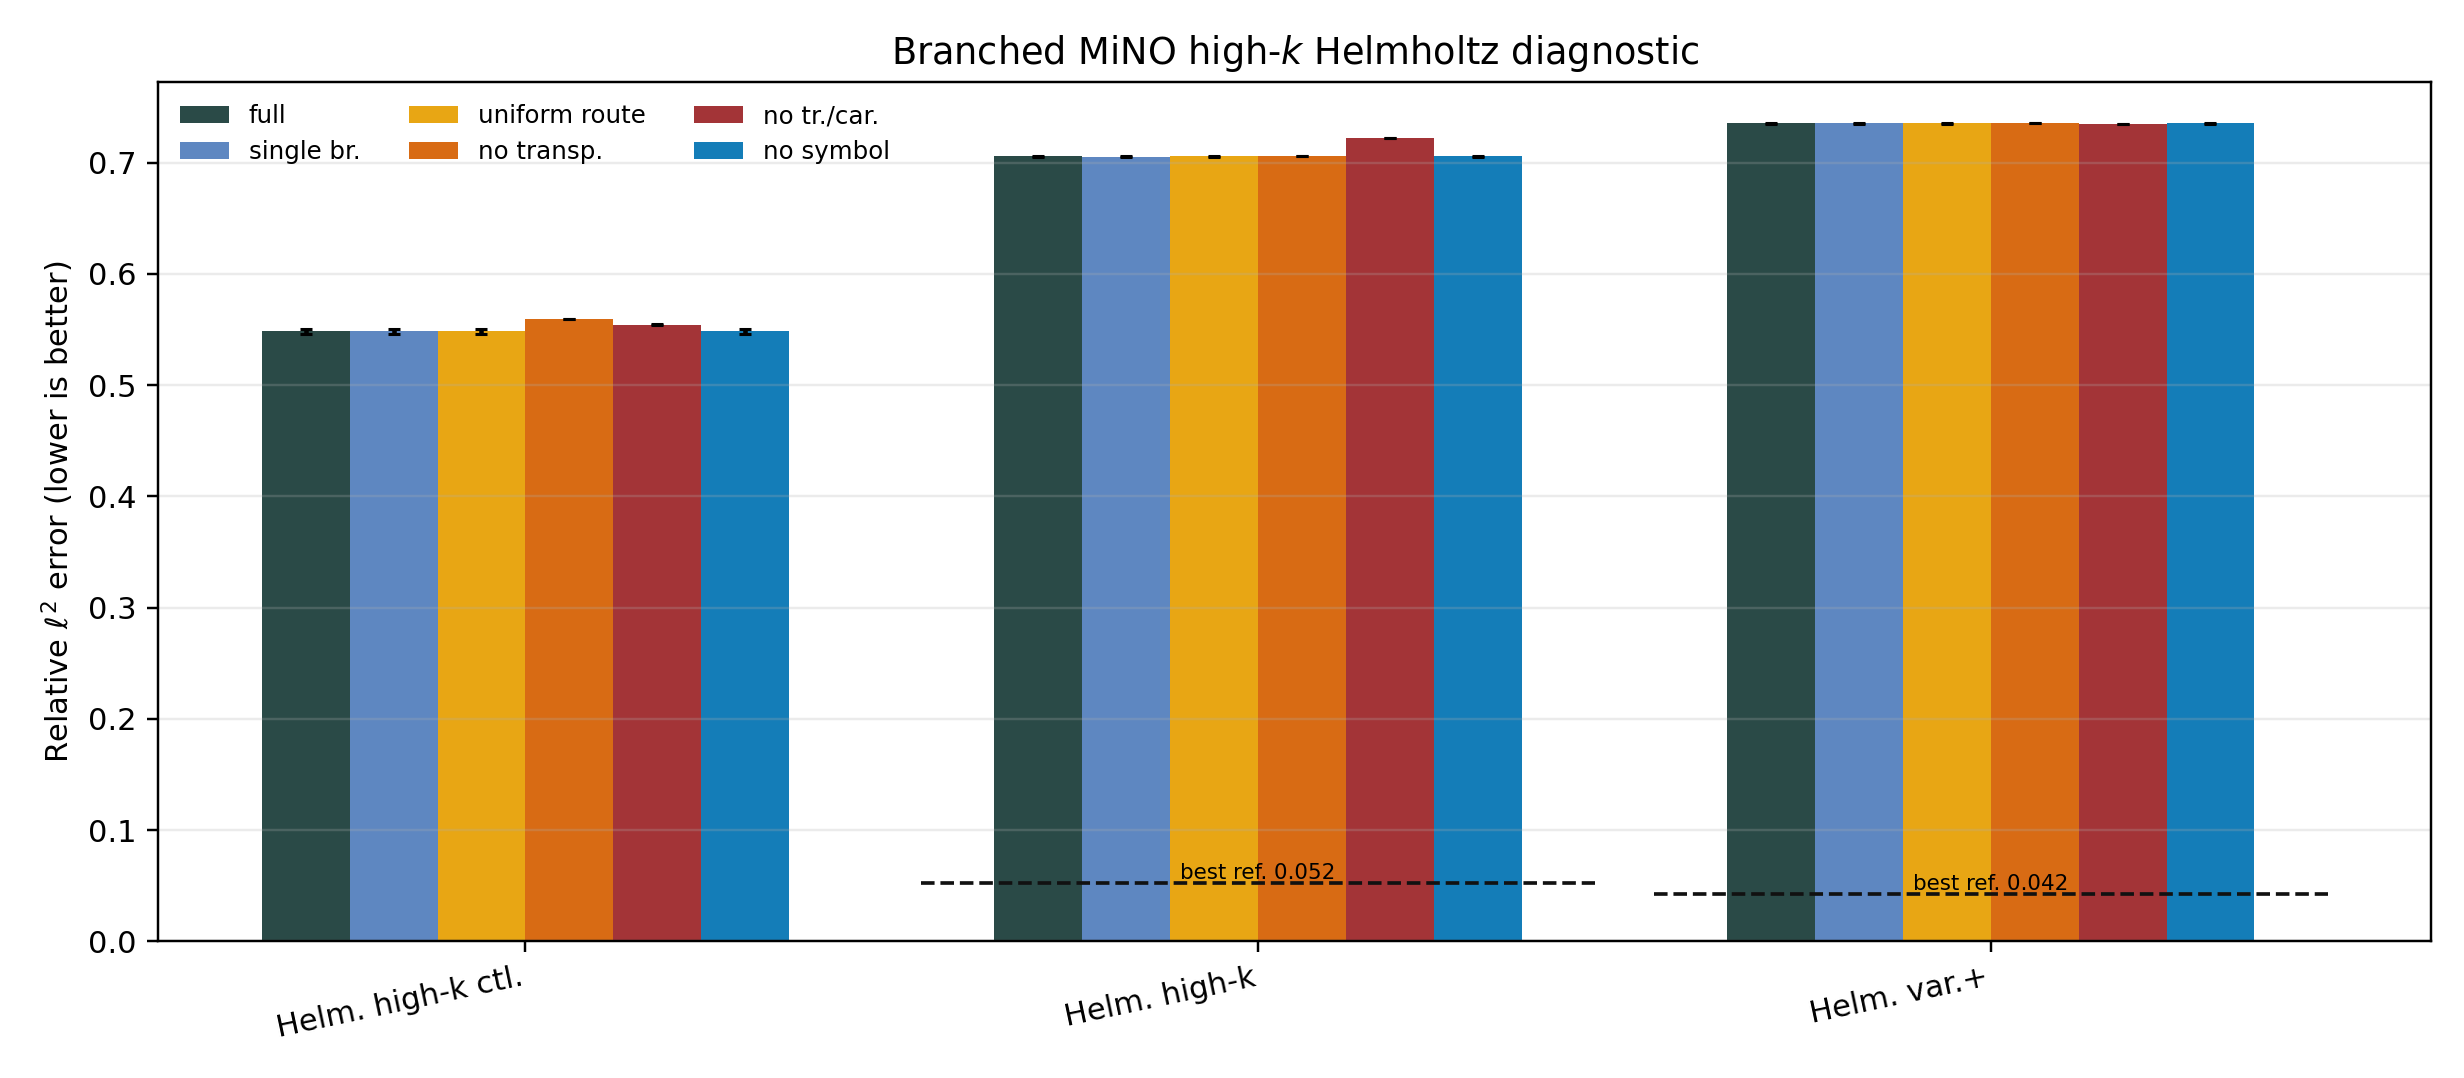
\includegraphics[width=\textwidth]{figures/helmholtz_branched_highk_relative_l2.png}
\caption{Branched \MiNO\ high-$k$ Helmholtz diagnostic.  The figure compares the full branched carrier-bound model against single-branch, uniform-routing, transport-removal, carrier-removal, and symbol-removal ablations under the local sample-capped protocol.  Dashed reference marks are imported baselines where available.}
\label{fig:helmholtz-branched-highk}
\end{figure}

\begin{figure}[t]
\centering
\begin{minipage}{0.49\linewidth}
\centering
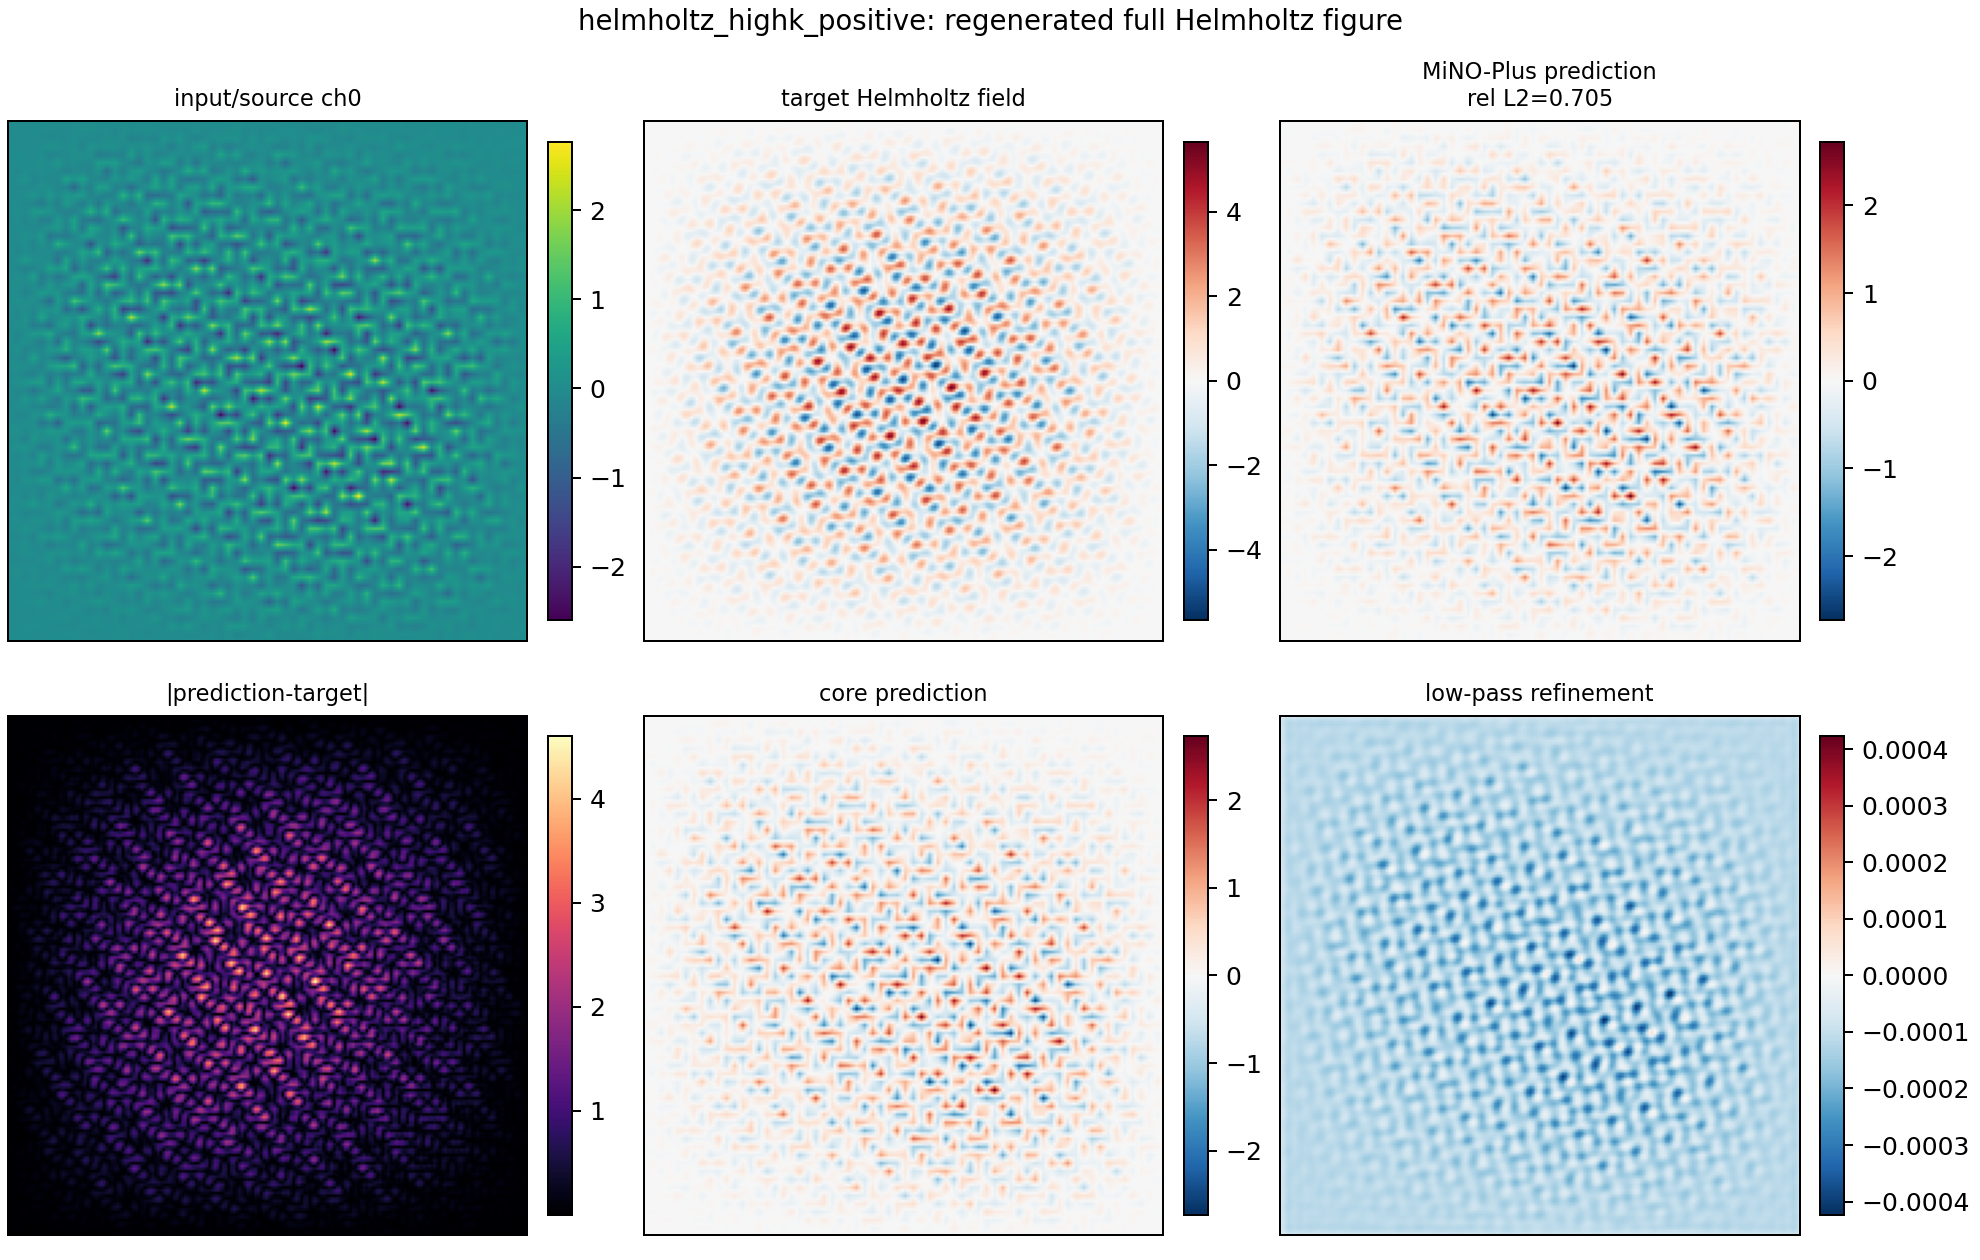
\includegraphics[width=\linewidth]{figures/helmholtz_highk_positive_seed7_sample0_anisotropic_gabor_full_L3.png}
\end{minipage}
\hfill
\begin{minipage}{0.49\linewidth}
\centering
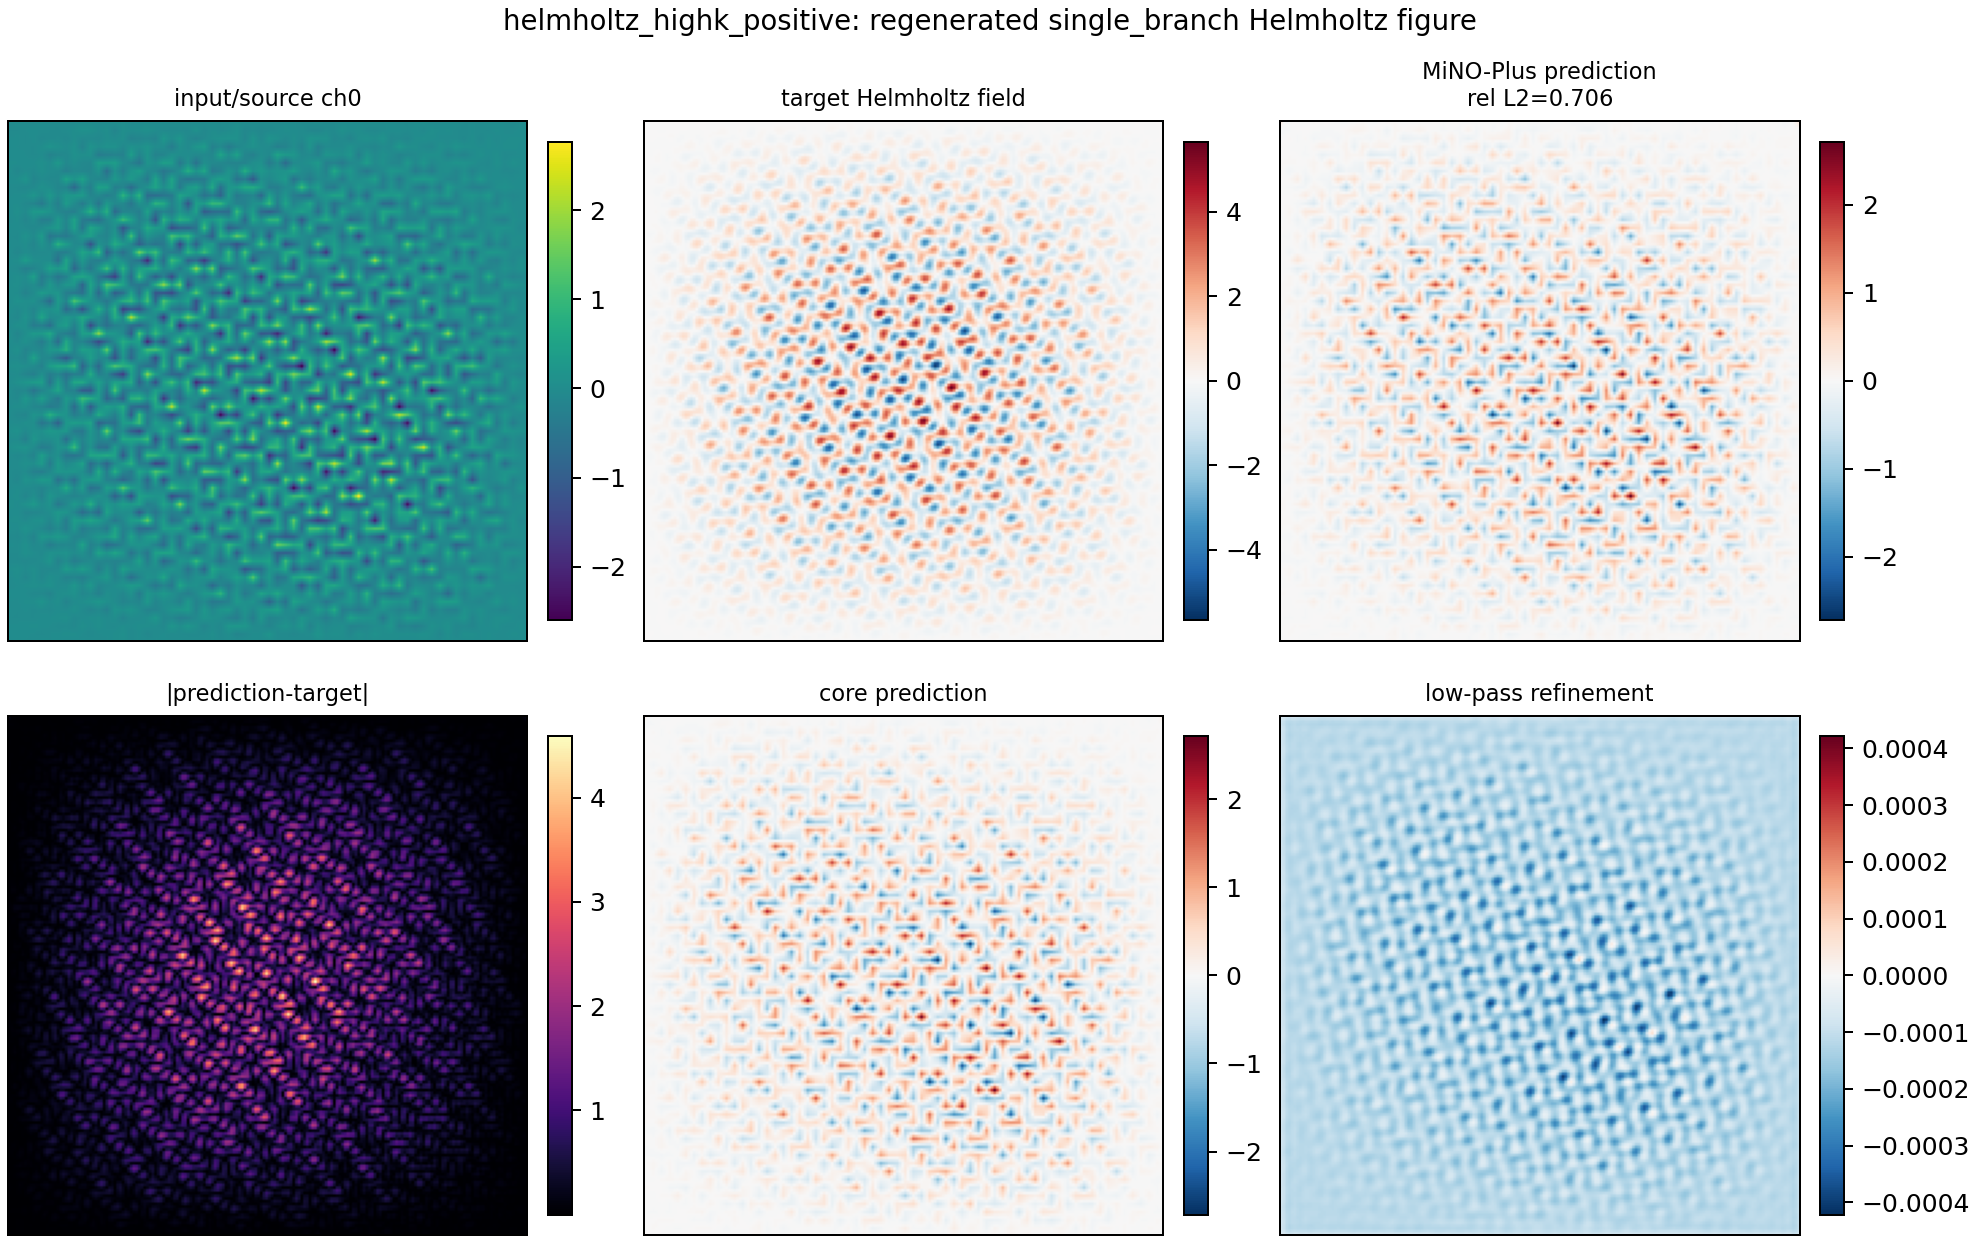
\includegraphics[width=\linewidth]{figures/helmholtz_highk_positive_seed7_sample0_anisotropic_gabor_single_branch_L3.png}
\end{minipage}
\caption{High-$k$ Helmholtz prediction panels for the sample-capped branched diagnostic.  Left: full $L=3$ branched model.  Right: forced single-branch control at the same budget and sample.  The nearly identical relative errors show that branch multiplicity alone leaves the main high-$k$ correction budget to the frame, router, phase/landing, and resolvent-symbol terms.}
\label{fig:helmholtz-branched-predictions}
\end{figure}

\subsection{Low-Budget Calculus-Regime Diagnostics}

The following panels are stress diagnostics for local-window Helmholtz and
synthetic Navier--Stokes profiles.  They are included to document boundary
conditions for future calculus hooks, not as main success claims.

\begin{figure}[t]
\centering
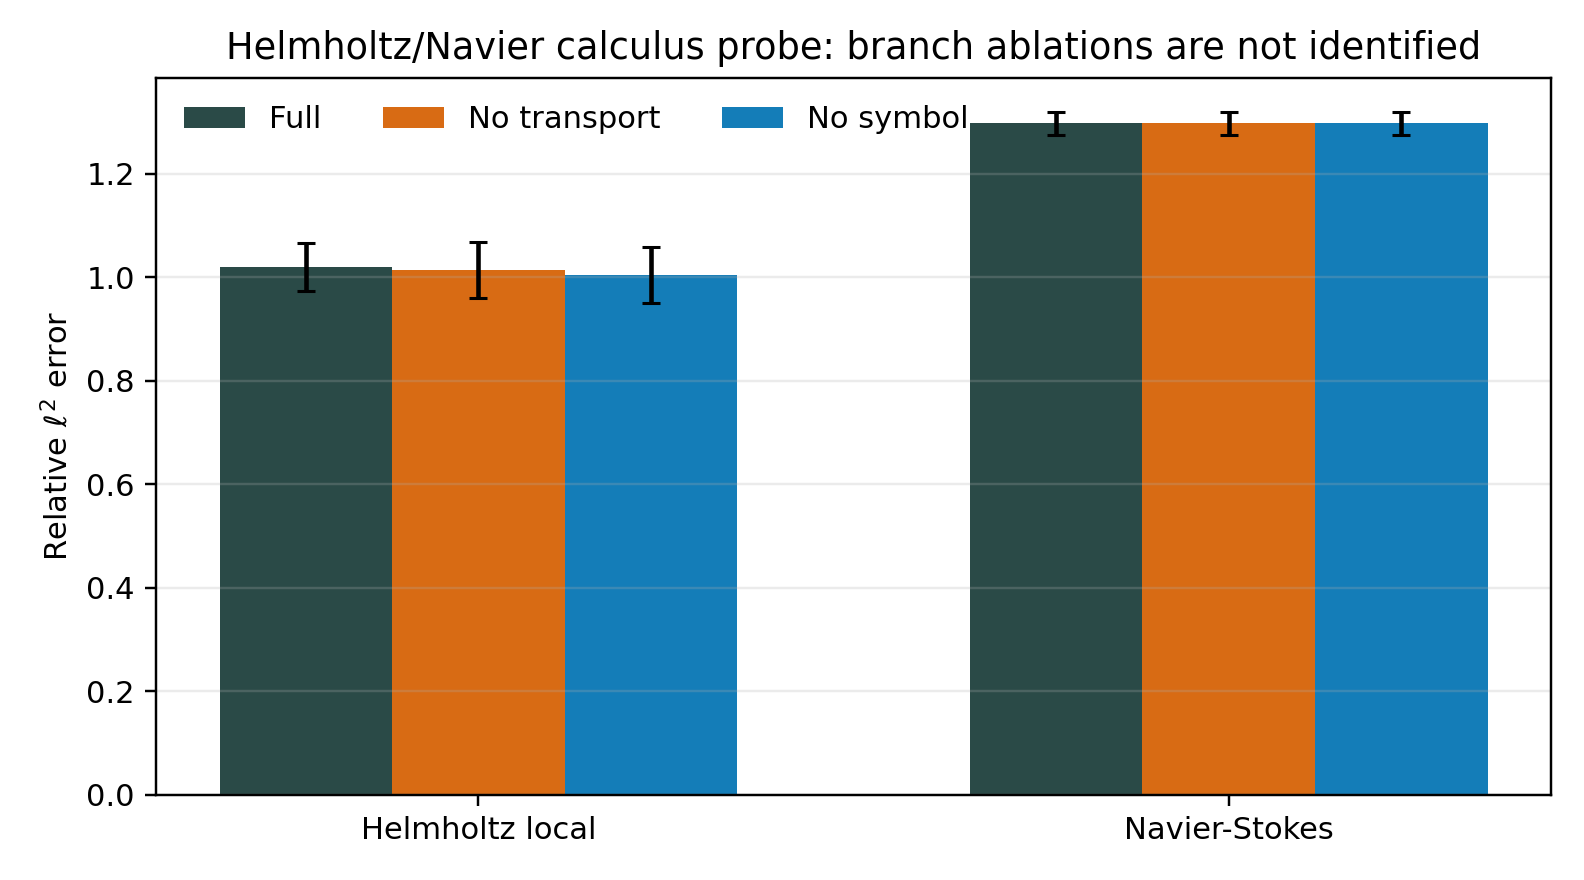
\includegraphics[width=0.82\textwidth]{figures/helmholtz_navier_calculus_probe.png}
\caption{Low-budget calculus-regime probe on local-window Helmholtz and synthetic Navier--Stokes.  Each row uses three seeds, twelve epochs, and restricted train/validation/test samples.  The nearly flat ablation bars identify which branch effects are not active at this scale and motivate the dedicated branch/resolvent and transport--diffusion profiles.}
\label{fig:helmholtz-navier-calculus-probe}
\end{figure}

\begin{figure}[t]
\centering
\begin{minipage}{0.49\linewidth}
\centering
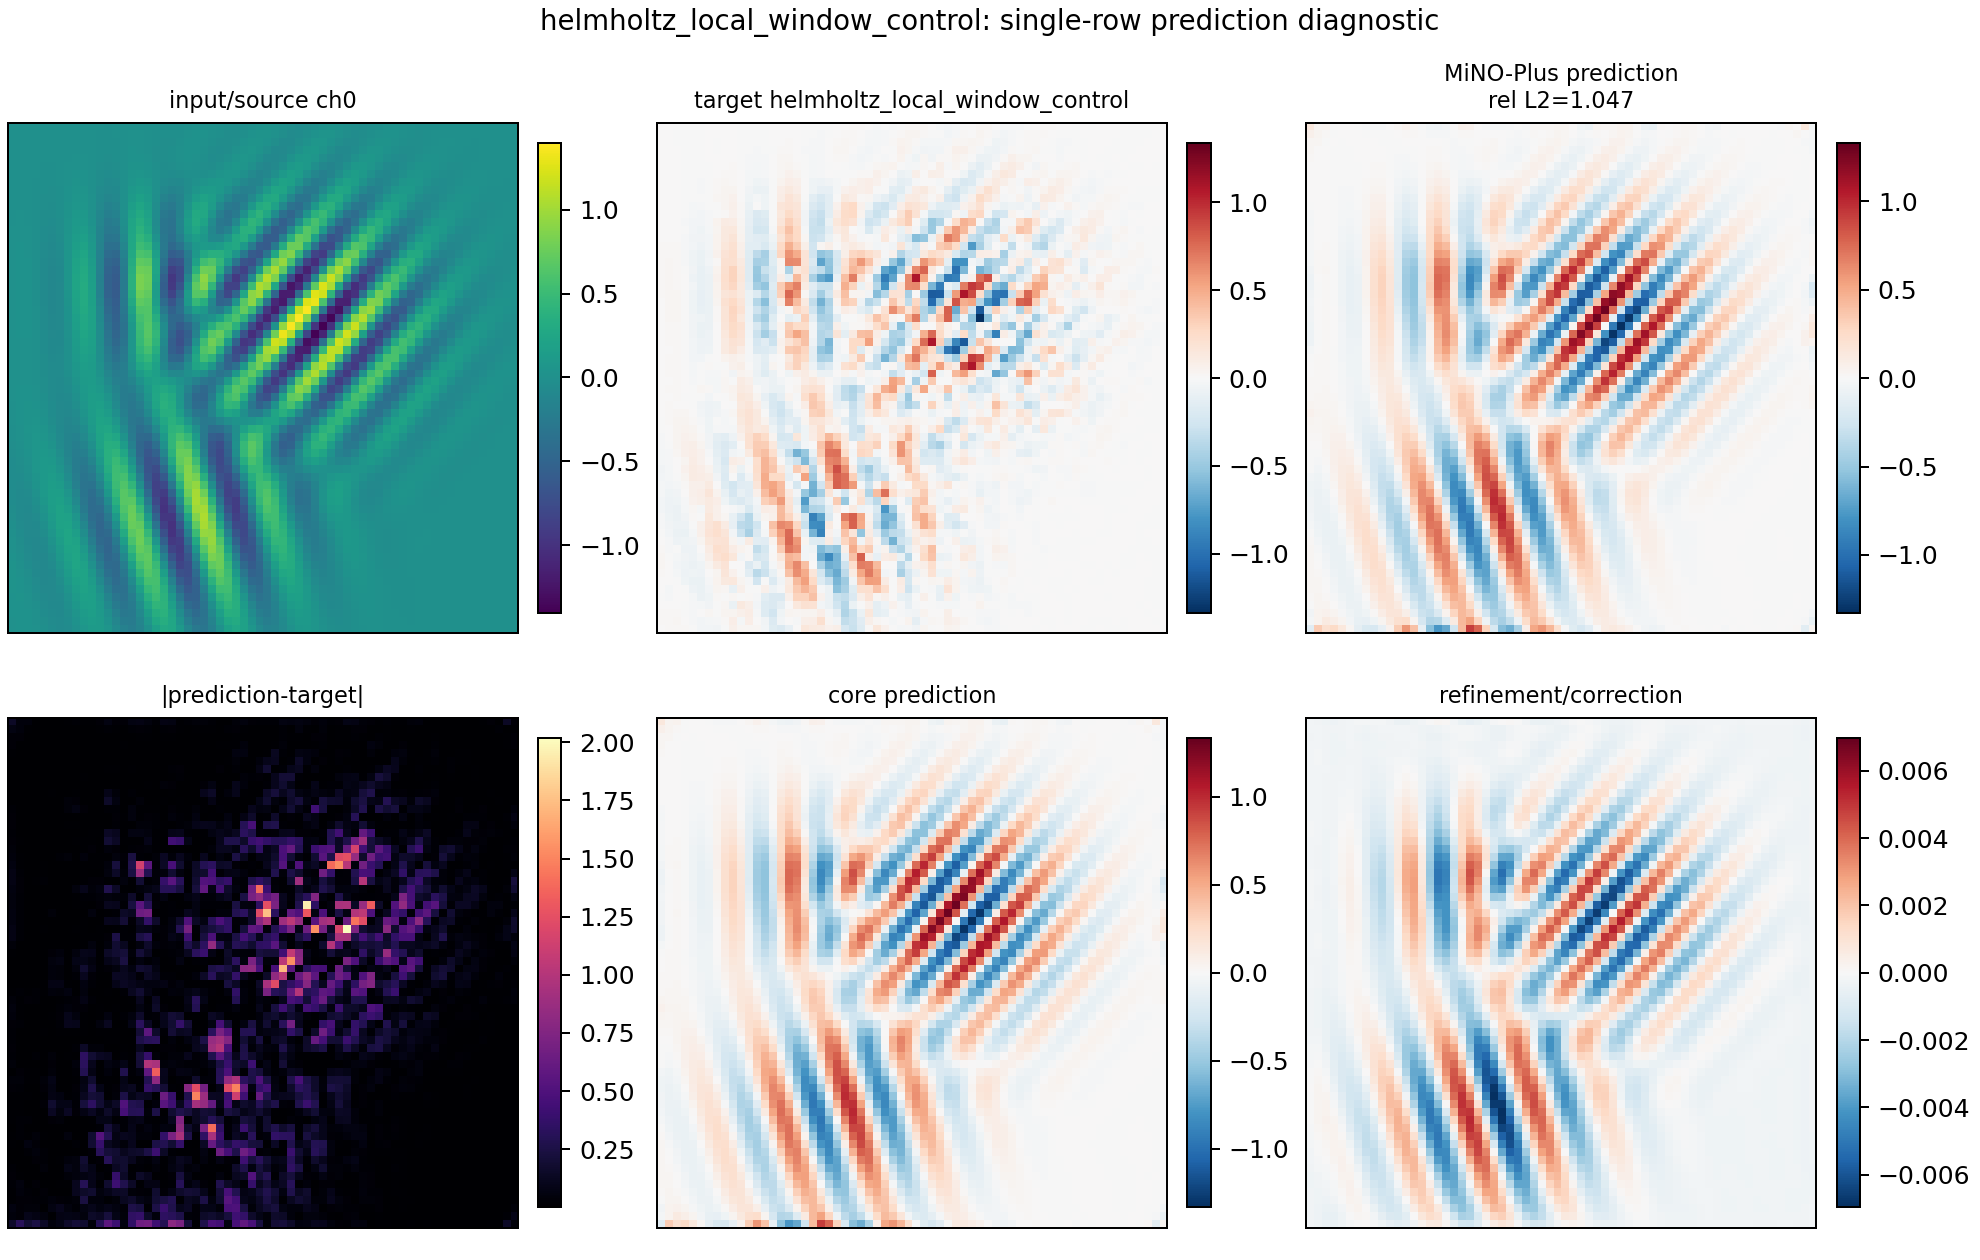
\includegraphics[width=\linewidth]{figures/helmholtz_local_window_prediction.png}
\end{minipage}
\hfill
\begin{minipage}{0.49\linewidth}
\centering
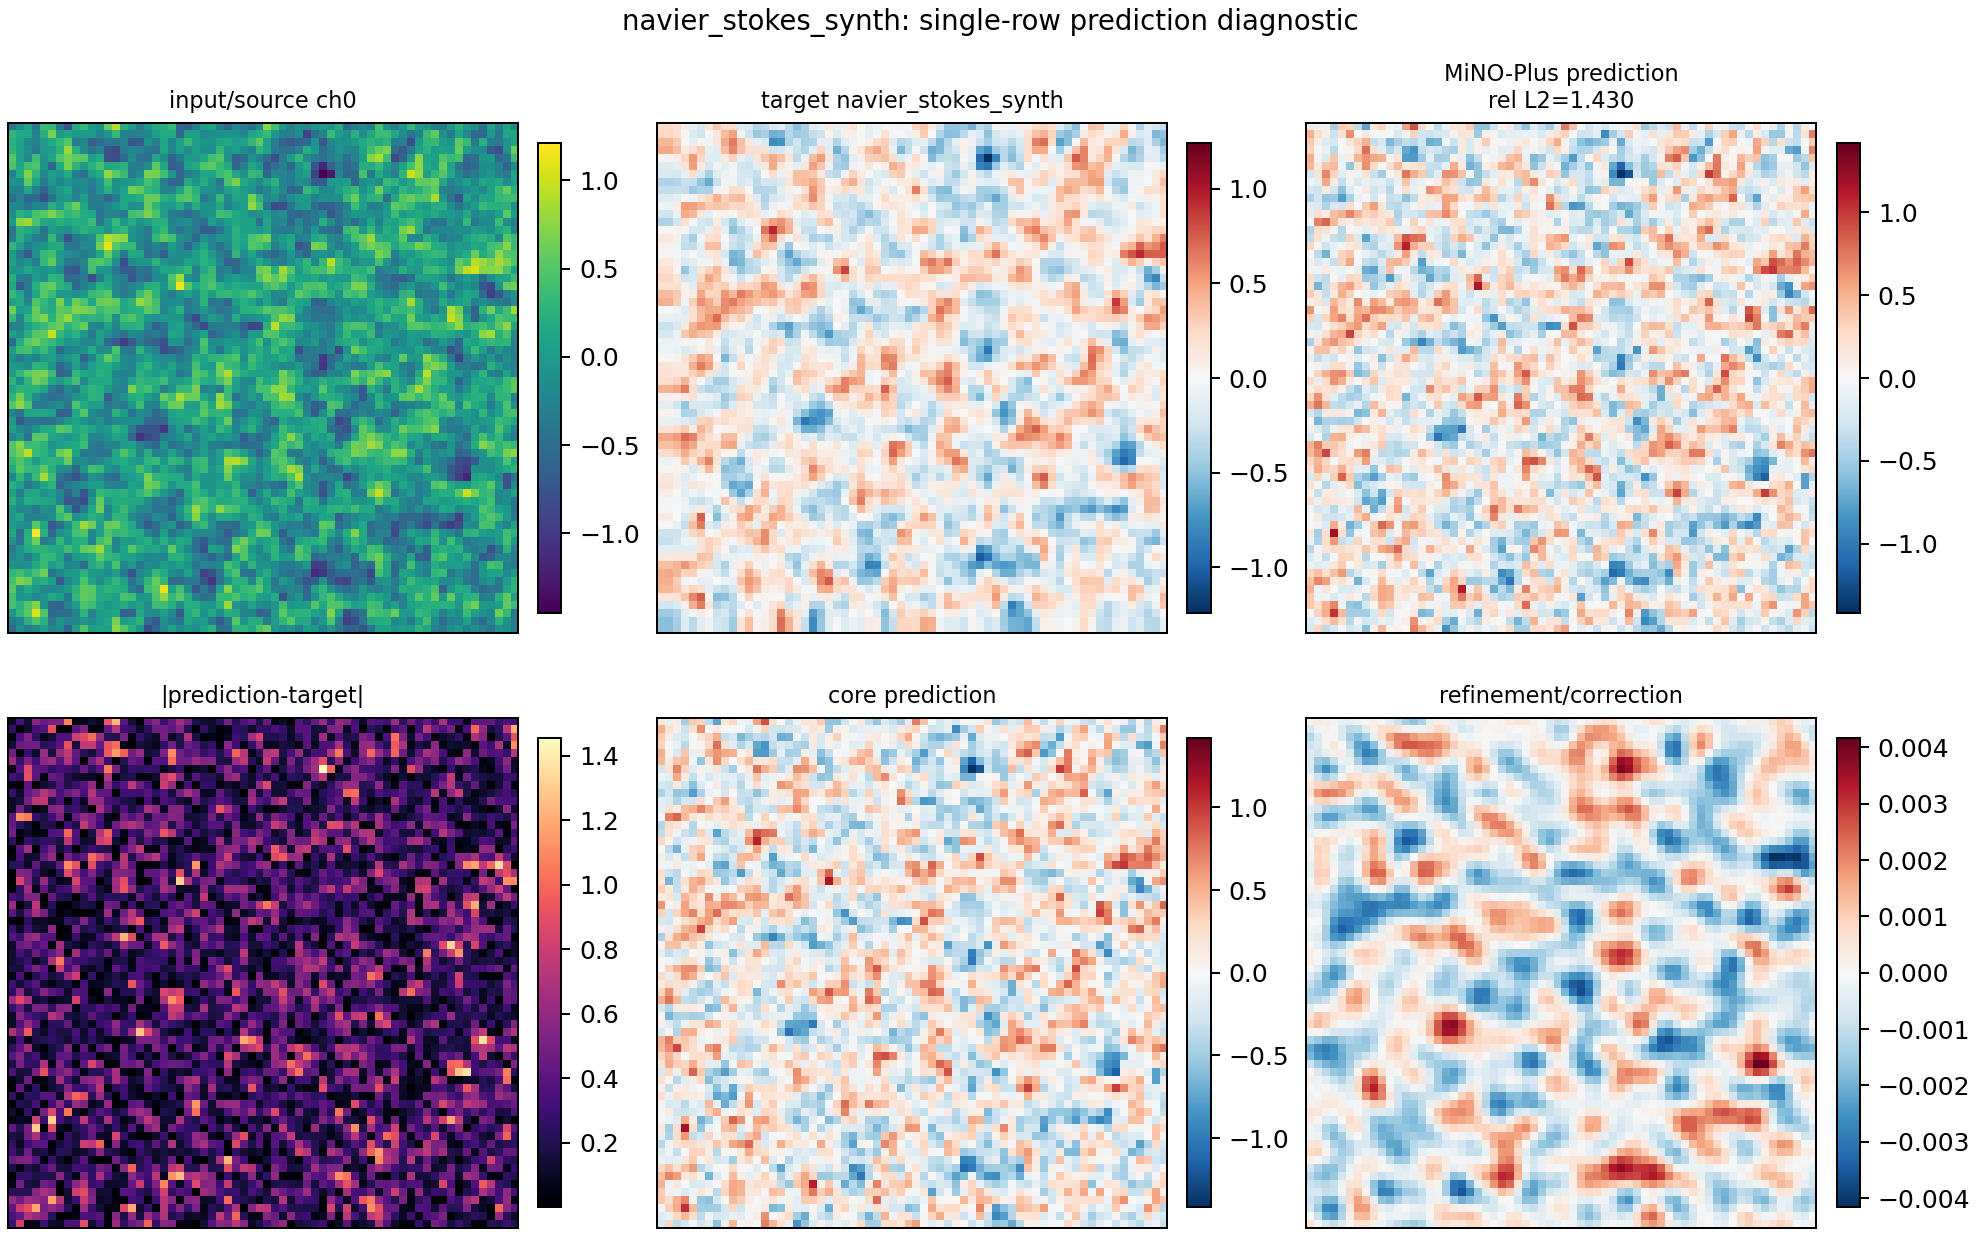
\includegraphics[width=\linewidth]{figures/navier_stokes_prediction.png}
\end{minipage}
\caption{Single-row prediction diagnostics for the same low-budget Helmholtz/Navier probe.  The panels visualize input, target, prediction, absolute error, core prediction, and refinement/correction for one held-out sample.  These rows show the regimes that motivate the next calculus hooks.}
\label{fig:helmholtz-navier-prediction-panels}
\end{figure}

\clearpage

\section{Machine-Proof Companion}
\label{app:formalization}

The Lean companion is intentionally finite.  It checks the landing layer reached after the classical microlocal estimates have produced finite packet tails, stencils, and budgets.  It does not formalize oscillatory integrals, stationary phase, or the full H\"ormander calculus.

\subsection{Lean Scope}

The Lean files in \codepath{lean/MiNO/Microlocal/} formalize:
\begin{itemize}
\item finite packet data structures and transported-symbol actions;
\item pointwise and $\ell^1$ finite propagation bounds;
\item bounded-stencil finite propagation;
\item finite approximation and identity-canonical reduction lemmas;
\item the global-scalar obstruction inequality;
\item semi-discrete transplantation and cross-resolution transfer;
\item canonical-tube, shell-counting, packet-tail, and abstract sparsity bridges;
\item finite packet-matrix tail accumulation;
\item restricted non-stationary-phase certificate handoff;
\item finite FIO/$\Psi$DO/smoothing branch composition;
\item finite packet-microscope ridge inclusion, fingerprint-budget stability,
finite Egorov budget expansion, composition-budget accumulation, and
learning-budget transfer for the extended theorem package.
\end{itemize}
This is the machine-checked finite part of the proof spine used by Sections~\ref{sec:theory}--\ref{sec:pde}.  The new $\ell^2$ packet-matrix Schur transfer is an elementary manuscript-level operator-norm step built on these finite row/column and tail objects; it is not advertised as a continuous Lean formalization.

\clearpage
\subsection{Proof-Status Inventory}

\begin{table}[!htbp]
\centering
\scriptsize
\setlength{\tabcolsep}{3pt}
\caption{Proof-status inventory for the manuscript.}
\label{tab:proofstatus}
\begin{tabular}{p{0.38\textwidth}p{0.24\textwidth}p{0.26\textwidth}}
\toprule
Claim layer & Status & Source \\
\midrule
Finite transported-symbol perturbation & fully formalized & Lean + Section~\ref{sec:theory} \\
Bounded-stencil finite propagation & fully formalized & Lean + Section~\ref{sec:theory} \\
Schur packet-matrix transfer & manuscript proof from finite row/column bounds & Theorem~\ref{thm:schur-packet-matrix} \\
Cross-resolution transfer & fully formalized & Lean + Section~\ref{sec:theory} \\
Canonical tube, shell count, packet tail & fully formalized finite bridge & Lean + Section~\ref{sec:continuous} \\
Packet-matrix tail accumulation & fully formalized finite bridge & Lean \codepath{PacketMatrix.lean} \\
Restricted non-stationary-phase handoff & formal finite wrapper with classical certificate input & Lean \codepath{NonstationaryPhase.lean} \\
Unified FIO/$\Psi$DO/smoothing composition & formal finite wrapper with classical input & Lean \codepath{UnifiedCalculus.lean} \\
Packet-microscope ridge inclusion and finite fingerprint/Egorov/composition budgets & fully formalized finite algebra & Lean \codepath{Flagship.lean} \\
Representation separation, fingerprint compiler stability, local Helmholtz packet budget & manuscript proof with classical packet/FIO input & Appendix~\ref{app:flagship-theorems} \\
Short-time half-wave off-graph decay & classical manuscript proof & Section~\ref{sec:continuous}, Appendix~\ref{app:continuous} \\
Abstract canonical-graph packet sparsity & classical derivation plus finite bridge & Section~\ref{sec:continuous} \\
Continuous transported-symbol reduction & classical manuscript proof & Section~\ref{sec:continuous}, Appendix~\ref{app:continuous} \\
Hamiltonian metadata consistency & manuscript proof & Proposition~\ref{prop:hamiltonian-metadata-consistency} \\
Microlocal Propagation Theorem for \MiNO-Core & classical continuous input + standard NN approximation + finite Lean bridge & Theorem~\ref{thm:wave-mino-core} \\
PDE specialization statements & manuscript-level derivations and modeling assumptions & Section~\ref{sec:pde} \\
\bottomrule
\end{tabular}
\end{table}

\subsection{Executable Certificates}

Two lightweight certificate paths accompany the Lean project.  The SymPy transport certificate expands the finite coefficient identity behind the transported-symbol bound.  The interval-style script checks concrete budget instances and writes the result to \codepath{certificates/interval\_check.json}.  These certificates are sanity checks for the finite algebra; they are not substitutes for the continuous microlocal argument.

\subsection{Next Formalization Targets}

The next useful Lean targets are weighted packet norms, confidence-weighted stencils, stronger finite packet-matrix residual operators, finite-to-asymptotic bridge lemmas indexed by the packet scale $h$, and finite matrix-norm versions of the Egorov and composition lemmas in Appendix~\ref{app:flagship-theorems}.  A more substantive proof-assistant target is a finite-frequency version of Calder\'on--Vaillancourt continuity for order-aware packet symbols, together with finite symplectic metadata maps and their canonical-defect estimates.  These targets are closer to the actual microlocal content than the elementary finite triangle inequalities, while still avoiding the full analytic burden of continuous oscillatory integrals. Full continuous microlocal formalization would require substantial new libraries for oscillatory integrals, pseudodifferential symbol classes, Hamiltonian flows, Sobolev spaces, and wavefront sets.


\bibliography{mino_refs}

\end{document}
